
\documentclass[
	fontsize=11pt, % Base font size
	twoside=false, % Use different layouts for even and odd pages (in particular, if twoside=true, the margin column will be always on the outside)
	%open=any, % If twoside=true, uncomment this to force new chapters to start on any page, not only on right (odd) pages
	%chapterprefix=true, % Uncomment to use the word "Chapter" before chapter numbers everywhere they appear
	%chapterentrydots=true, % Uncomment to output dots from the chapter name to the page number in the table of contents
	numbers=noenddot, % Comment to output dots after chapter numbers; the most common values for this option are: enddot, noenddot and auto (see the KOMAScript documentation for an in-depth explanation)
	%draft=true, % If uncommented, rulers will be added in the header and footer
	%overfullrule=true, % If uncommented, overly long lines will be marked by a black box; useful for correcting spacing problems
]{kaobook}

% Set the language
\usepackage[english]{babel} % Load characters and hyphenation
\usepackage[english=british]{csquotes} % English quotes

\usepackage{bm}


% txfonts/pxfonts

% Load packages for testing
\usepackage{blindtext}
%\usepackage{showframe} % Uncomment to show boxes around the text area, margin, header and footer
%\usepackage{showlabels} % Uncomment to output the content of \label commands to the document where they are used

% Load the bibliography package
\usepackage{styles/kaobiblio}
\addbibresource{biblio.bib} % Bibliography file

% Load mathematical packages for theorems and related environments. NOTE: choose only one between 'mdftheorems' and 'plaintheorems'.
\usepackage{styles/mdftheorems}
%\usepackage{styles/plaintheorems}


\graphicspath{{images/}} % Paths in which to look for images

% \RequirePackage{times}

\DeclareMathOperator{\cA}{{\mathcal A}}
\DeclareMathOperator{\cB}{{\mathcal B}}
\DeclareMathOperator{\cC}{{\mathcal C}}
\DeclareMathOperator{\cD}{{\mathcal D}}
\DeclareMathOperator{\cE}{{\mathcal E}}
\DeclareMathOperator{\cF}{{\mathcal F}}
\DeclareMathOperator{\cG}{{\mathcal G}}
\DeclareMathOperator{\cM}{{\mathcal M}}
\DeclareMathOperator{\cN}{{\mathcal N}}
\DeclareMathOperator{\cP}{{\mathcal P}}
\DeclareMathOperator{\cX}{{\mathcal X}}
\DeclareMathOperator{\cY}{{\mathcal Y}}
\DeclareMathOperator{\cZ}{{\mathcal Z}}

\DeclareMathOperator{\bA}{{\boldsymbol A}}
\DeclareMathOperator{\bB}{{\boldsymbol B}}
\DeclareMathOperator{\bC}{{\boldsymbol C}}
\DeclareMathOperator{\bD}{{\boldsymbol D}}
\DeclareMathOperator{\bE}{{\boldsymbol E}}
\DeclareMathOperator{\bF}{{\boldsymbol F}}
\DeclareMathOperator{\bG}{{\boldsymbol G}}
\DeclareMathOperator{\bH}{{\boldsymbol H}}
\DeclareMathOperator{\bI}{{\boldsymbol I}}
\DeclareMathOperator{\bJ}{{\boldsymbol J}}
\DeclareMathOperator{\bK}{{\boldsymbol K}}
\DeclareMathOperator{\bL}{{\boldsymbol L}}
\DeclareMathOperator{\bM}{{\boldsymbol M}}
\DeclareMathOperator{\bN}{{\boldsymbol N}}
\DeclareMathOperator{\bO}{{\boldsymbol O}}
\DeclareMathOperator{\bP}{{\boldsymbol P}}
\DeclareMathOperator{\bQ}{{\boldsymbol Q}}
\DeclareMathOperator{\bR}{{\boldsymbol R}}
\DeclareMathOperator{\bS}{{\boldsymbol S}}
\DeclareMathOperator{\bT}{{\boldsymbol T}}
\DeclareMathOperator{\bU}{{\boldsymbol U}}
\DeclareMathOperator{\bV}{{\boldsymbol V}}
\DeclareMathOperator{\bW}{{\boldsymbol W}}
\DeclareMathOperator{\bX}{{\boldsymbol X}}
\DeclareMathOperator{\bY}{{\boldsymbol Y}}
\DeclareMathOperator{\bZ}{{\boldsymbol Z}}

\DeclareMathOperator{\ba}{{\boldsymbol a}}
\DeclareMathOperator{\bb}{{\boldsymbol b}}
\DeclareMathOperator{\bc}{{\boldsymbol c}}
\DeclareMathOperator{\bd}{{\boldsymbol d}}
\DeclareMathOperator{\be}{{\boldsymbol e}}
% \DeclareMathOperator{\bf}{{\boldsymbol f}}
\DeclareMathOperator{\bg}{{\boldsymbol g}}
\DeclareMathOperator{\bh}{{\boldsymbol h}}
\DeclareMathOperator{\bi}{{\boldsymbol i}}
\DeclareMathOperator{\bj}{{\boldsymbol j}}
\DeclareMathOperator{\bk}{{\boldsymbol k}}
\DeclareMathOperator{\bl}{{\boldsymbol l}}
% \DeclareMathOperator{\bm}{{\boldsymbol m}}
\DeclareMathOperator{\bn}{{\boldsymbol n}}
\DeclareMathOperator{\bo}{{\boldsymbol o}}
\DeclareMathOperator{\bp}{{\boldsymbol p}}
\DeclareMathOperator{\bq}{{\boldsymbol q}}
\DeclareMathOperator{\br}{{\boldsymbol r}}
\DeclareMathOperator{\bs}{{\boldsymbol s}}
\DeclareMathOperator{\bt}{{\boldsymbol t}}
\DeclareMathOperator{\bu}{{\boldsymbol u}}
\DeclareMathOperator{\bv}{{\boldsymbol v}}
\DeclareMathOperator{\bw}{{\boldsymbol w}}
\DeclareMathOperator{\bx}{{\boldsymbol x}}
\DeclareMathOperator{\by}{{\boldsymbol y}}
\DeclareMathOperator{\bz}{{\boldsymbol z}}

\DeclareMathOperator{\bLambda}{{\boldsymbol \Lambda}}

\DeclareMathOperator{\bone}{\boldsymbol 1}

\DeclareMathOperator{\beps}{\boldsymbol \varepsilon}
\DeclareMathOperator{\bSigma}{\boldsymbol \Sigma}

\DeclareMathOperator{\tr}{tr}
\DeclareMathOperator{\diag}{diag}
\DeclareMathOperator{\im}{im}
\DeclareMathOperator{\mode}{mode}
\DeclareMathOperator{\rank}{rank}
\DeclareMathOperator{\med}{med}
\DeclareMathOperator{\pen}{pen}
\DeclareMathOperator{\inte}{int}
\DeclareMathOperator{\dom}{dom}


\DeclareMathOperator{\ber}{Bernoulli}
\DeclareMathOperator{\bet}{Beta}
\DeclareMathOperator{\bin}{Binomial}
\DeclareMathOperator{\chisq}{ChiSq}
\DeclareMathOperator{\expo}{Exponential}
\DeclareMathOperator{\fis}{Fisher}
\DeclareMathOperator{\gam}{Gamma}
\DeclareMathOperator{\mul}{Multinomial}
\DeclareMathOperator{\nor}{Normal}
\DeclareMathOperator{\stu}{Student}
\DeclareMathOperator{\uni}{Uniform}

\DeclareMathOperator{\new}{new}



\DeclareMathOperator{\sigmoid}{sigmoid}
\DeclareMathOperator{\leb}{Lebesgue}
\DeclareMathOperator*{\argmin}{argmin}
\DeclareMathOperator*{\argmax}{argmax}

\DeclareMathOperator*{\spa}{span}
\DeclareMathOperator{\proj}{proj}
\DeclareMathOperator{\cov}{cov}

\newcommand{\eps}{\varepsilon}

\renewcommand{\P}{\mathbb P}
\newcommand{\E}{\mathbb E}
\newcommand{\R}{\mathbb R}
\newcommand{\N}{\mathbb N}
\newcommand{\var}{\mathbb V}

\newcommand{\wh}{\widehat}
\newcommand{\wt}{\widetilde}

\newcommand{\ind}[1]{\mathbf 1_{#1}}
\newcommand{\grad}{\nabla}


\newcommand{\mgeq}{\succcurlyeq}
\newcommand{\mleq}{\preccurlyeq}
\newcommand{\goes}{\rightarrow}
\newcommand{\go}{\rightarrow}

\newcommand{\norm}[1]{\| #1 \|}
\newcommand{\inr}[1]{\langle #1 \rangle}

\newcommand{\gopro}{\overset{\P}{\rightarrow}}
\newcommand{\goas}{\overset{\text{as\ }}{\rightarrow}}
\newcommand{\goqr}{\overset{\text{$L^2$\ }}{\rightarrow}}
\newcommand{\gosto}{\leadsto}


% \newcommand{\lest}{ \underset{\text{st}}{\leq}}
\newcommand{\lest}{\preceq}
% \newcommand{\gest}{\underset{\text{st}}{\qeq}}
\newcommand{\gest}{\succeq}



% \makeindex[columns=3, title=Alphabetical Index, intoc] % Make LaTeX produce the files required to compile the index

% \makeglossaries % Make LaTeX produce the files required to compile the glossary

% \makenomenclature % Make LaTeX produce the files required to compile the nomenclature

% Reset sidenote counter at chapters
%\counterwithin*{sidenote}{chapter}

%----------------------------------------------------------------------------------------

\begin{document}

%----------------------------------------------------------------------------------------
%	BOOK INFORMATION
%----------------------------------------------------------------------------------------

\titlehead{Some stuff about statistics}
\subject{Lecture notes for the ENS course of Statistics}

\title[Some stuff about Statistics]{Some stuff about Statistics}
% \subtitle{Customise this page according to your needs}

\author[St\'ephane Ga\"iffas"]{St\'ephane Ga\"iffas\thanks{}}

\date{\today}

\publishers{}

%----------------------------------------------------------------------------------------

\frontmatter % Denotes the start of the pre-document content, uses roman numerals

%----------------------------------------------------------------------------------------
%	OPENING PAGE
%----------------------------------------------------------------------------------------

%\makeatletter
%\extratitle{
%	% In the title page, the title is vspaced by 9.5\baselineskip
%	\vspace*{9\baselineskip}
%	\vspace*{\parskip}
%	\begin{center}
%		% In the title page, \huge is set after the komafont for title
%		\usekomafont{title}\huge\@title
%	\end{center}
%}
%\makeatother

%----------------------------------------------------------------------------------------
%	COPYRIGHT PAGE
%----------------------------------------------------------------------------------------

% \makeatletter
% \uppertitleback{\@titlehead} % Header

% \lowertitleback{
% 	\textbf{Disclaimer}\\
% 	You can edit this page to suit your needs. For instance, here we have a no copyright statement, a colophon and some other information. This page is based on the corresponding page of Ken Arroyo Ohori's thesis, with minimal changes.
	
% 	\medskip
	
% 	\textbf{No copyright}\\
% 	\cczero\ This book is released into the public domain using the CC0 code. To the extent possible under law, I waive all copyright and related or neighbouring rights to this work.
	
% 	To view a copy of the CC0 code, visit: \\\url{http://creativecommons.org/publicdomain/zero/1.0/}
	
% 	\medskip
	
% 	\textbf{Colophon} \\
% 	This document was typeset with the help of \href{https://sourceforge.net/projects/koma-script/}{\KOMAScript} and \href{https://www.latex-project.org/}{\LaTeX} using the \href{https://github.com/fmarotta/kaobook/}{kaobook} class.
	
% 	The source code of this book is available at:\\\url{https://github.com/fmarotta/kaobook}
	
% 	(You are welcome to contribute!)
	
% 	\medskip
	
% 	\textbf{Publisher} \\
% 	First printed in May 2019 by \@publishers
% }
% \makeatother

%----------------------------------------------------------------------------------------
%	DEDICATION
%----------------------------------------------------------------------------------------

% \dedication{
% 	The harmony of the world is made manifest in Form and Number, and the heart and soul and all the poetry of Natural Philosophy are embodied in the concept of mathematical beauty.\\
% 	\flushright -- D'Arcy Wentworth Thompson
% }

%----------------------------------------------------------------------------------------
%	OUTPUT TITLE PAGE AND PREVIOUS
%----------------------------------------------------------------------------------------

% Note that \maketitle outputs the pages before here

% If twoside=false, \uppertitleback and \lowertitleback are not printed
% To overcome this issue, we set twoside=semi just before printing the title pages, and set it back to false just after the title pages
\KOMAoptions{twoside=semi}
\maketitle
\KOMAoptions{twoside=false}

%----------------------------------------------------------------------------------------
%	PREFACE
%----------------------------------------------------------------------------------------

\chapter*{Preface}
\addcontentsline{toc}{chapter}{Preface} % Add the preface to the table of contents as a chapter


The aim of this course is, as the title indicated, to learn some stuff about statistics, and to try to exhibit some good looking mathematics from this field of applied mathematics, beyond convincing you that statistics are useful\sidenote{We won't list here, exhaustively, the numerous fields that make a regular use of mathematical statistics: marketing, medicine and more broadly health, finance, insurance, banking, etc.}

We will try to provide, all along the course, at material featuring 60\% of classical and unavoidable material from a course about statistics, and 40\% of more recent research results and some open questions.

The tentative agenda for the course is as follows:

\begin{itemize}
 	\item Modelization and the main statistical inference problems (estimation, confidence regions and tests)
 	\item Gaussian vectors and the Gaussian linear model
 	\item Theoretical guarantees and the optimality of least-squares
 	\item Estimation methods: methods of moments, maximum likelihood and other things
 	\item Exponential models and generalized linear models, logistic regression (optimal rates and some open questions)
 	\item Tests and multiple tests
 \end{itemize} 

% I am of the opinion that every \LaTeX\xspace geek, at least once during 
% his life, feels the need to create his or her own class: this is what 
% happened to me and here is the result, which, however, should be seen as 
% a work still in progress. Actually, this class is not completely 
% original, but it is a blend of all the best ideas that I have found in a 
% number of guides, tutorials, blogs and tex.stackexchange.com posts. In 
% particular, the main ideas come from two sources:

% \begin{itemize}
% 	\item \href{https://3d.bk.tudelft.nl/ken/en/}{Ken Arroyo Ohori}'s 
% 	\href{https://3d.bk.tudelft.nl/ken/en/nl/ken/en/2016/04/17/a-1.5-column-layout-in-latex.html}{Doctoral 
% 	Thesis}, which served, with the author's permission, as a backbone 
% 	for the implementation of this class;
% 	\item The 
% 		\href{https://github.com/Tufte-LaTeX/tufte-latex}{Tufte-Latex 
% 			Class}, which was a model for the style.
% \end{itemize}

% The first chapter of this book is introductive and covers the most 
% essential features of the class. Next, there is a bunch of chapters 
% devoted to all the commands and environments that you may use in writing 
% a book; in particular, it will be explained how to add notes, figures 
% and tables, and references. The second part deals with the page layout 
% and design, as well as additional features like coloured boxes and 
% theorem environments.

% I started writing this class as an experiment, and as such it should be 
% regarded. Since it has always been indended for my personal use, it may 
% not be perfect but I find it quite satisfactory for the use I want to 
% make of it. I share this work in the hope that someone might find here 
% the inspiration for writing his or her own class.

\begin{flushright}
	\textit{St\'ephane Ga\"iffas}
\end{flushright}


%----------------------------------------------------------------------------------------
%	TABLE OF CONTENTS & LIST OF FIGURES/TABLES
%----------------------------------------------------------------------------------------

\begingroup % Local scope for the following commands

% Define the style for the TOC, LOF, and LOT
%\setstretch{1} % Uncomment to modify line spacing in the ToC
%\hypersetup{linkcolor=blue} % Uncomment to set the colour of links in the ToC
\setlength{\textheight}{23cm} % Manually adjust the height of the ToC pages

% Turn on compatibility mode for the etoc package
\etocstandarddisplaystyle % "toc display" as if etoc was not loaded
\etocstandardlines % toc lines as if etoc was not loaded

\tableofcontents % Output the table of contents

% \listoffigures % Output the list of figures

% Comment both of the following lines to have the LOF and the LOT on different pages
% \let\cleardoublepage\bigskip
% \let\clearpage\bigskip

% \listoftables % Output the list of tables

\endgroup

%----------------------------------------------------------------------------------------
%	MAIN BODY
%----------------------------------------------------------------------------------------

\mainmatter % Denotes the start of the main document content, resets page numbering and uses arabic numbers
\setchapterstyle{kao} % Choose the default chapter heading style


\setchapterpreamble[u]{\margintoc}
\chapter{Statistical models}
\label{chap:statistical_models}

Let us start with the most classical and simplest statistical experiment: the coin toss.
We toss a coin $n$ times, and we model each toss by a random variable in $\{ 0, 1 \}$, where we decide that $1$ means that the toss ended up with heads (so that $0$ means tails).
To each toss is associated a random variable, leading to random variables $X_1, \ldots, X_n$  valued in $\{ 0, 1 \}$, where $X_i$ encodes the outcome of the $i$-th toss.
Each $X_i$ has distribution $\ber(p)$ for $p \in [0, 1]$, where $p$ corresponds to the probability that a coin toss gives heads, namely $\P(X_i = 1)$.%
\sidenote{The notation $\ber(p)$ corresponds to the \emph{Bernoulli distribution}: we will write $X \sim \ber(p)$ whenever $X \in \{ 0, 1\}$ and $\P(X = 1) = p = 1 - \P(X = 0)$.
Another way to obtain a $\ber$ distribution is by setting $X_i = \ind{Y_i \in A}$ where $Y_1, \ldots, Y_n$ are random variables valued in a probability space $(E, \cE)$, with $A \in \cE$, so that $X_i \sim \ber(p)$ with $p = \P(Y_i \in A)$.}
We assume that the $X_i$ are \emph{independent} (since the outcome of the tosses are physically unrelated), and since we are tossing the same coin each time, we assume that these outcomes have the same distribution (meaning that $p$ is constant along the tosses).
Therefore, we assume that $X_1, \ldots, X_n$ are \emph{iid}.%
\sidenote{From now on, iid will stand for \emph{independent and identically distributed}. More about this fundamental assumption will follow.}

\section{Probabilities and statistics} % (fold)
\label{sec:probability_versus_statistics}

Since we assume that the reader is familiar with the field of probabilities, we start this chapter with a comparison between what we do in probabilities and what we do in statistics for the $\ber(p)$ model described above.

\todo{remettre $S_n$ partout, faut pas deconner}


\paragraph{Probabilities.} % (fold)

% paragraph probability (end)
In the field of probabilities, we suppose that $p \in (0, 1)$ is known, and we study the properties of the sequence $(X_i)_{i \geq 1}$. 
For instance, we know that the distribution of $S_n = \sum_{i=1}^n X_i$ is $\bin(n, p)$,  
namely that $\P(S_n = k) = \binom{n}{k} p^k (1 - p)^{n-k}$ for $k \in \{0, \ldots, n\}$.%
\sidenote{Where $\binom{n}{k}$ is the $(n, k)$ binomial coefficient given by $\frac{n!}{k! (n - k)!}$.}
It is easy to see that $\E(S_n) = n p$ and that $\var(S_n) = np (1 - p)$, where $\E(\cdot)$ and $\var(\cdot)$ stand respectively for the expectation and the variance.%
\sidenote{The linearity of the expectation gives $\E(S_n) = n \E(X_1) = np$ since the $X_i$ are identically $\ber(p)$ distributed, and, since the $X_i$ are iid, we know that $\var(S_n) = n \var(X_1) = n p (1 - p)$.}%
We can study the asymptotic properties of $S_n$, such as
\begin{equation}
	\label{eq:lln-binomial}
	\frac{S_n}{n} \goas p
\end{equation}
and
\begin{equation}
	\label{eq:tcl-binomial}
	\sqrt n \Big(\frac{S_n}{n} - p\Big) \leadsto \nor(0, p(1-p))
\end{equation}
as $n \rightarrow +\infty$, where $\nor(\mu, \sigma^2)$ stands for the Gaussian distribution with expectation $\mu$ and variance $\sigma^2$.%
\sidenote{The notation $X_n \goas X$ stands for the \emph{almost sure} convergence of $X_n$ towards $X$ while $X_n \leadsto X$ stands for the convergence of $X_n$ towards $X$ in distribution.}.
Note that statement~\eqref{eq:lln-binomial} comes from the law of large numbers, while~\eqref{eq:tcl-binomial} comes from the central limit theorem.
In the field of probabilities, the object of interest would be the \emph{random variable} $S_n$, that we study knowing the value of $p$.
In particular, if we replace the $\ber(p)$ distribution by the \emph{Rademacher distribution} $\text{Rademacher}(p)$ where $\P(X_i = 1) = 1 - \P(X_i = -1) = p$, the random variable $S_n$ becomes a \emph{random walk} for which many things can be said, depending on the value of $p$.%
\sidenote{But such things are way beyond the topic of this book, let us just cite~\cite{lawler2010random} as a reference on the study of the random walk and its importance in the field of probability theory.}

\paragraph{Statistics.} % (fold)

In statistics, for the $\ber(p)$ example, we don't really care about $S_n$, but we do care about $p$.
We assume that $p$ is \emph{unknown}, and we want to find out things about it.
This objective is called \emph{statistical inference} of the \emph{parameter} $p$.
For instance, we would like to know if $p=1/2$ or not, in order to find out if the coin is well-balanced and not rigged.
The random variables $X_1, \ldots, X_n$ (and $S_n$) live on some probability space $(\Omega, \cA, \P)$, but we don't really care about it either in statistics.
We will always assume, in statistics, that each \emph{observed} outcome $x_i \in \{ 0, 1 \}$ of a coin toss is a \emph{realization} of the random variable $X_i$, namely that
\begin{equation*}
	x_i = X_i(\omega)
\end{equation*}
for some \emph{event} $\omega \in \Omega$.
The realizations $x_i$ are also called \emph{data} or \emph{samples} or \emph{observations}.
But, actually, we will also refer to the random variables $X_i$ in the same way, as \emph{data}, \emph{samples} or \emph{observations}, since we won't manipulate the $x_i$ mathematically,%
\sidenote{nothing can be done with them... it's just deterministic zeros and ones}%
while we will work a lot with the random variables $X_1, \ldots, X_n$.
In statistics, we can do whatever we want with $X_1, \ldots, X_n$ in order to say things about $p$, but we will \emph{never} assume $p$ to be known.%
\sidenote{The parameter $p$ will quickly become a mathematical variable that we will use in equations, in order to perform calculus for instance. Therefore, we will use the specific notation $p_0$ for the ground truth parameter, namely $X_1 \sim \ber(p_0)$, while $p$ will be used as a generic parameter. A statistical parameter will usually be denoted as $\theta$, while the ground truth parameter will be denoted as $\theta_0$ when necessary.}
We will construct measurable functions of $(X_1, \ldots, X_n)$ that do not depend on $p$, these are called \emph{statistics}, in order to tell things about the unknown parameter $p$.
The object of interest in the field of statistics is, therefore, rather the \emph{distribution of the observations} than the observations themselves.


\section{Statistical models and experiences} % (fold)
\label{sec:statistical_models_and_experiences}

Let us consider another very classical problem: the election poll problem, where a population of size $N$ vote for one of two candidates $A$ and $B$.
There are $N_A$ people voting for $A$ while $N - N_A$ vote for $B$, and we want to know about $\theta_0 = N_A / N$.
We perform of poll including $n \ll N$ voters and obtain observations $x_1, \ldots, x_n \in \{ 0, 1 \}$, where $x_i = 0$ (resp. $x_i = 1$) means that voter $i$ votes for $B$ (resp. $A$).
In this problem, both $N_A$ and $N$ are so large that we can suppose that
\begin{equation*} 
	(x_1, \ldots, x_n) = (X_1(\omega), \ldots, X_n(\omega))
\end{equation*}
for some $\omega \in \Omega$, where all $X_i : (\Omega, \cA, \P) \rightarrow (\{0, 1\}, \cP(\{ 0, 1\})$ for $i=1, \ldots,, n$ are such that $X_i \sim \ber(\theta_0)$.
Let's look a little bit at all these mathematical objects. 
In statistics, we are mainly only interested by the fact that the observations are valued in $(\{0, 1\}, \cP(\{ 0, 1\})$ and that the distribution is $\P_{X_i} = \ber(\theta_0)$, which is fully described by its parameter $\theta_0 \in (0, 1)$.
Once again, we don't really care about $(\Omega, \cA, \P)$ in statistics.

\paragraph{Statistical model.}

The \emph{statistical model} for $X = (X_1, \ldots, X_n) \in \{0, 1\}^n$ is the family of distributions
\begin{equation*}
	\big\{ \P_\theta^{\otimes n} : \theta \in (0, 1) \big\}	= \big\{ \ber(\theta)^{\otimes n} : \theta \in (0, 1) \big\},
\end{equation*}
which is a family indexed by $\theta \in (0, 1)$.
The notation $\P^{\otimes n} = \P \otimes \cdots \otimes \P$ stands for the tensor product, namely $\P^{\otimes n}(A_1 \times \cdots \times A_n) = \prod_{i=1}^n \P(A_i)$ for any $A_i \in \cA$, $i=1, \ldots, n$.%
\sidenote{In this book, we will quickly forget to write $\P^{\otimes n}$ and we will write simply $\P$, when computations are clear enough, to avoid overloaded notations.}
When we say that this is a statistical model for $X$, we assume that there exist $\theta_0 \in (0, 1)$ such that $X \sim \ber(\theta_0)$.
Once again, let us insist on the following: we do whatever we want with $X_1, \ldots, X_n$ but never with $\theta_0$, which is the unknown parameter.

\paragraph{Another (naive) example.}

Let us consider the problem of the quality of production of screws. 
The dimensions of the screws must satisfy some strong constraints, for instance their length must match quite accurately some fixed size.%
\sidenote{The author of this book does not know anything about screws.}%
\begin{marginfigure}%
	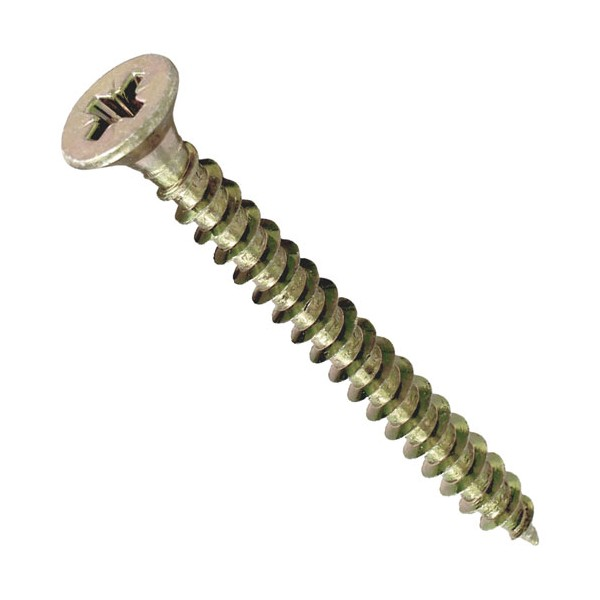
\includegraphics{screw.jpg}%
	\caption{I can't resist the temptation of showing you a screw, so here it is.}%
\end{marginfigure}%
Millions of screws come out of the production chain, and we can't test all of them.
Therefore, we need to assess the production quality by selecting at random a small set of $n$ screws, and we measure their lengths $x_1, \ldots, x_n$.
Since these lengths are highly concentrated around the theoretical desired length $\mu$, and since production errors are usually small, we decide to choose a Gaussian model: we assume that $x_i = X_i(\omega)$ for $X_i \sim \nor(\mu, \sigma^2)$, where $\sigma^2$ corresponds to a variance coming from the (hopefully) small production errors.

\emph{A model is a simplification of the reality.} For this example, we make the following modeling assumptions.
\begin{description}
	\item[Distribution choice.] We choose the distribution $\nor(\mu, \sigma^2)$ for the lengths. So, we implicitly assume that the true underlying distribution of the lengths is \emph{symmetrical} and highly \emph{concentrated} around $\mu$. This may or may not be realistic.%
	\sidenote{A real random variable $X$ is \emph{symmetrical} whenever $\P_X = \P_{-X}$. This means that $\P(X \leq -x) = \P(X \geq x)$ so that $F(-x) = 1 - F(x_-)$ if $F$ is the distribution function of $X$. Also, if $X$ has a density $f$ with respect to the Lebesgue measure, then $f$ is an even function.}
	\item[The iid assumption.] We will assume also that $X_i$ are iid. What this means in practice is that we need to very careful in the way we select the screws coming out of the production lines: for instance, we should pick screws all along a week or a month, at different times, and not all from the same production line, in order to avoid time and machine biases.
\end{description}

Once again, a statistical model is always a simplification and an approximation of the truth.
By \emph{truth} we mean the true distribution $\P_{(X_1, \ldots, X_n)}$ of $(X_1, \ldots, X_n)$.
For instance, the $\nor(0, 1)$ distribution has density $\phi(x) = e^{-x^2/2} / \sqrt{2 \pi}$ supported on $\R$. 
This means that realizations of a $\nor(0, 1)$ distribution can take any value in $\R$, while real samples are usually bounded.
However, we can prove that if $Z \sim \nor(0, 1)$, then $\Phi(x) := \P(Z \leq x)$ satisfies
\begin{marginfigure}
	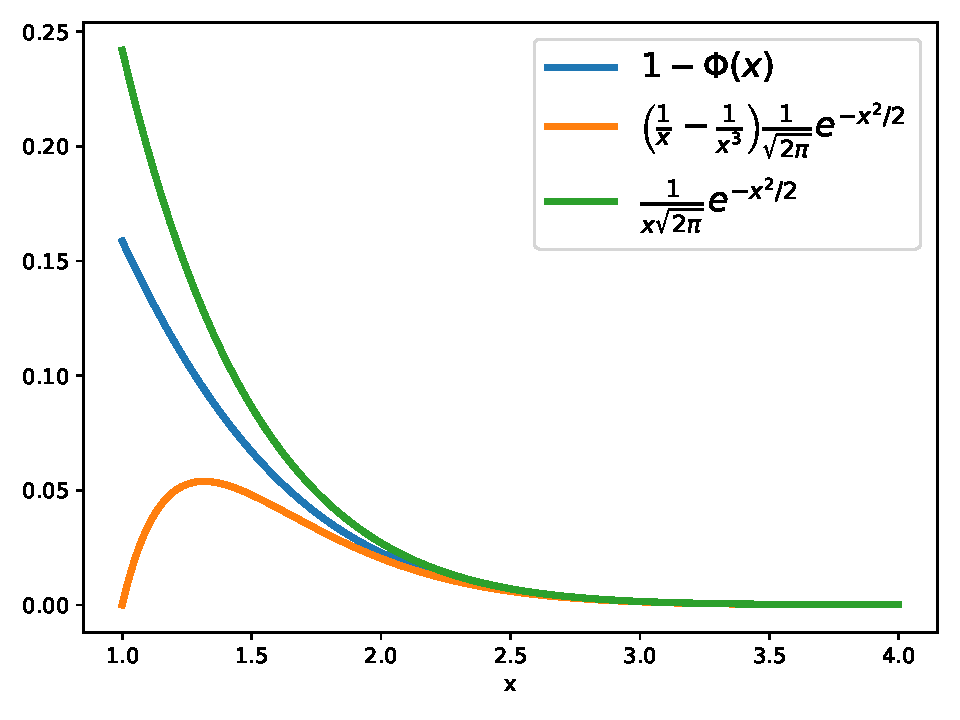
\includegraphics{images/gaussian_queue.pdf}
	\caption{Illustration of the lower and upper bounds proposed in Equation~\eqref{eq:gaussian_queue}.}
\end{marginfigure}%
\begin{equation}
	\label{eq:gaussian_queue}
	\Big( \frac 1x - \frac{1}{x^3} \Big) \frac{1}{\sqrt{2\pi}} e^{-x^2 / 2} \leq 1 - \Phi(x) \leq \frac{1}{x \sqrt{2 \pi}} e^{-x^2 / 2}
\end{equation}
for any $x > 1$, which means that the \emph{queue}%
\sidenote{The \emph{queue} of a real random variable $Z$ is the function $x \mapsto \P(Z > x)$.}%
of the $\nor$ distribution is very tight.
For $x=6$ for instance, we have $\P(Z > x) \leq 10^{-9}$: we will actually never see realizations of $\nor(0, 1)$ outside of $[-6, 6]$, and rarely outside of $[-3, 3]$.
\begin{definition}
	\label{def:statistical_experiment}
	A \emph{statistical experiment} consists of the following two things:
	\begin{itemize}
		\item A \emph{random object} $X$ valued in a probability space $(E, \cE)$
		\item A \emph{family of distributions} $\cP = \{ P_\theta : \theta \in \Theta\}$ on $(E, \cE)$.
	\end{itemize}
	We suppose that $\P_X = \P \circ X^{-1} \in \cP$. We say that $\cP$ is a \emph{statistical model} for $X$ and we will denote the statistical experiment as $(X, \cP)$.
	We call $\Theta$ the \emph{set of parameters} of the model.
\end{definition}
\marginnote{We call $X$ a \emph{random object} in Definition~\ref{def:statistical_experiment} to stress that it can be a real random variable, a random vector, a random matrix, among other things.}
The random variable $X : (\Omega, \cA, \P) \rightarrow (E, \cE)$ has distribution $\P_X = \P \circ X^{-1}$ which is the probability image of $\P$ by $X$ on $(\Omega, \cA)$.
We will always suppose that there is a family $\{ \P_\theta : \theta \in \Theta\}$ on $(\Omega, \cA)$ that induce $\{ P_\theta : \theta \in \Theta\}$ on $(E, \cE)$ and we will use the notations
\begin{equation*}
	P_\theta(A) = \P_\theta(X \in A) = \P_\theta[ \{ \omega \in \Omega : X(\omega) \in A \}] \quad \forall A \in \cE.
\end{equation*}
Let us insist on the fact that $(\Omega, \cA, \P)$ is a purely mathematical build that has no interest in statistics.
We could even assume that $X$ is the identity function and that $(\Omega, \cA) = (E, \cE)$.
Because of the transfer formula
\begin{equation*}
	\int f(X(\omega)) \P_\theta(d \omega) = \int f(x) P_\theta(dx),
\end{equation*}
we can work only with $P_\theta$ and forget about $\P_\theta$ and the space $(\Omega, \cA)$.

We will often work with a space of finite-dimensional parameters $\Theta \subset \R^d$, which corresponds to the setting  of a \emph{parametric} model, but this space can be much more complicated (it can be a set of functions with some smoothness properties for instance, such a case is covered by a field called \emph{non-parametric} statistics).
We will use the notation
\begin{equation*}
	\E_Q f(Y) := \int f(y) Q(dy)
\end{equation*}
where we implicitly assume, when computing this expectation, that $Y \sim Q$, and whenever $Q = P_\theta$, we will shorten this notation as follows:
\begin{equation*}
	\E_\theta f(X) := \E_{\P_\theta} f(X) = \int f(x) P_\theta(dx).
\end{equation*}
We will never work on $(\Omega, \cA, \P)$ but rather on $(E, \cE)$ and with the family $\cP$ (the statistical model).
\marginnote{We will quickly forget to distinguish between $\P_\theta$ and $P_\theta$ and between $\P_\theta^{\otimes n}$ and $P_\theta^{\otimes n}$. And, once again, since we are particularly lazy, we will also write $P_\theta$ instead of $P_\theta^{\otimes n}$, when there is little doubt about what we are computing.}
\begin{definition}[Sampled statistical experiment]
We have observations $X = (X_1, \ldots, X_n)$ with $X_i$ iid and $\cP = \{ P_\theta^{\otimes n} : \theta \in \Theta\}$, namely for $A = \prod_{i=1}^n A_i$ we have
\begin{align*}
	P_\theta^{\otimes n}(A) &= \P_\theta^{\otimes n}( (X_1, \ldots, X_n) \in A_1 \times \cdots \times A_n) \\
	&= \prod_{i=1}^n \P_\theta(X_i \in A_i) = \prod_{i=1}^n P_\theta(A_i).
\end{align*}
\end{definition}

\section{Statistics}
\label{sec:statistics}

Now, let us go back to the $\ber(\theta)$ experiment.
Let us first recall that for this experiment we have iid samples $X = (X_1, \ldots, X_n)$, that
$(E, \cE) = (\{0, 1\}^n, \cP(\{0, 1\}^n))$ and that $P_\theta^{\otimes n} = \ber(\theta)^{\otimes n}$ with $\Theta = (0, 1)$.
Intuitively, an ``equivalent'' experiment is $S := \sum_{i=1}^n X_i$ and $(E, \cE) = (\{ 0, \ldots, n\}, \cP(\{0, \ldots, n\}))$ with $\Theta = (0, 1)$.
Let us observe that
\begin{equation}
	\label{eq:X_cond_S}
	\begin{split}
	\P_\theta (X_1 = x_1, \ldots, X_n = x_n | S = k) &= 
	\frac{\theta^k (1 - \theta)^{n-k}}{\binom{n}{k} \theta^k (1 - \theta)^{n-k}} \\
	&= \frac{1}{\binom{n}{k}}		
	\end{split}
\end{equation}
whenever $x_i \in \{ 0, 1 \}$ for $i=1, \ldots, n$ and $k = \sum_{i=1}^n x_i$, while $\P_\theta (X_1 = x_1, \ldots, X_n = x_n | S = k) = 0$ otherwise.
This proves that the conditional distribution of $(X_1, \ldots, X_n) | S$ \emph{does not depend} on $\theta$.
If we know $S$, then we can, \emph{without knowing} $\theta$, build a ``copy'' $X' = (X_1', \ldots, X_n')$ of the original sample $X$, in the sense that $X'$ has the same distribution as $X$.
This is simply achieved, as indicated by~\eqref{eq:X_cond_S}, by choosing the positions of the $S=k$ ones (among $n$ ones and zeros) uniformly at random.
This means that $X$ does not bring more information about $\theta$ than $S$, and that that $S$ is somehow ``sufficient'' from a statistical point of view.
Such a random variable is called a \emph{sufficient statistic}.
We really need at this point to tell the reader what a \emph{statistic} is.
\marginnote{Let us recall the Doob lemma. Let $X$ and $Y$ be two random variables on the same probability space. Then $Y$ is $X$-measurable (namely measurable with respect to the $\sigma$-field $\sigma(X)$ generated by $X$) if and only if there exists a measurable function $f$ such that $Y = f(X)$.}
\begin{definition}
	Given a statistical experiment $(X, \{ P_\theta : \theta \in \Theta \})$, we call \emph{statistic} any $X$-measurable function that does not depend on~$\theta$.
	A statistic is therefore a quantity that we can compute using data only.
\end{definition}
For the $\ber(\theta)$ experiment, we will look for statistics of $X$ allowing to infer the unknown parameter $\theta$.
We already now that we can restrict ourselves to statistics of $S$ instead of $X$, since $S$ is  sufficient.

\section{Identifiable models} % (fold)

The only source of information about $\theta$ available to us about is $X$, through its distribution $P_{\theta}$.
So, in order to infer $\theta$, we need, at least, to be able to recover $\theta$ given $P_\theta$.
We will therefore often require that the model is \emph{identifiable}, as defined below.
\begin{definition}
	We say that a model $\cP = \{ P_\theta : \theta \in \Theta \}$ is \emph{identifiable} whenever the function $\Theta \rightarrow \cP$ given by $\theta \mapsto P_\theta$
	is \emph{injective}.
\end{definition}
Identifiability is a necessary requirement when one wants to perform statistical inference.
If $\theta \mapsto P_\theta$ is not injective, then there is no way to find back $\theta$ from $X \sim P_\theta$.

\begin{example}
	\label{ex:identifiabiliy}
	Obviously, $\theta \mapsto \ber(\theta)$ is injective on $(0, 1)$ and similarly $x \mapsto \ber(\sigmoid(x))$ is injective on $\R$.
	A stupid example is $\mu \mapsto \nor(\mu^2, 1)$ on $\R$, which corresponds to a non-identifiable model.
\end{example}
In Example~\ref{ex:identifiabiliy}, we used the sigmoid function given by $\sigmoid(x) = 1 / (1 + e^{-x})$ for any $x \in \R$.%
\sidenote{The sigmoid function is heavily used in statistics and machine learning, we will come back to it later in the book.}
Identifiability is generally a property that we ensure by choosing and parametrizing correctly the considered statistical model.
An interesting example of \emph{non-identifiable} model is given by \emph{mixture models}, such as the Gaussian mixture model, where we consider a distribution on $\R^d$ with density
\sidenote{In the paramatrization of the Gaussian mixture we have expectations $\mu_k \in \R^d$ that correspond to the centroids of the clusters, we have covariances $\bSigma_k \in \R^{d \times d}$ such that $\bSigma_k \succ 0$, which means that $\bSigma_k$ is a symmetric and positive matrix, that parametrizes the shape cluster $k$ around its centroid and finally we have $\pi_k \geq 0$ that are such that $\sum_{k=1}^K \pi_k = 1$ and parametrize the relative population of each cluster.}%
\begin{align*}
	f_\theta(x) &= \sum_{k=1}^K \pi_k \phi_{\mu_k, \bSigma_k}(x) \\ 
	&=: \sum_{k=1}^K \frac{\pi_k }{\sqrt{(2 \pi)^d \det (\bSigma_k)}} 
	\exp\Big( -\frac 12 (x - \mu_k)^\top \bSigma_k^{-1} (x - \mu_k) \Big)
\end{align*}
\begin{marginfigure}
	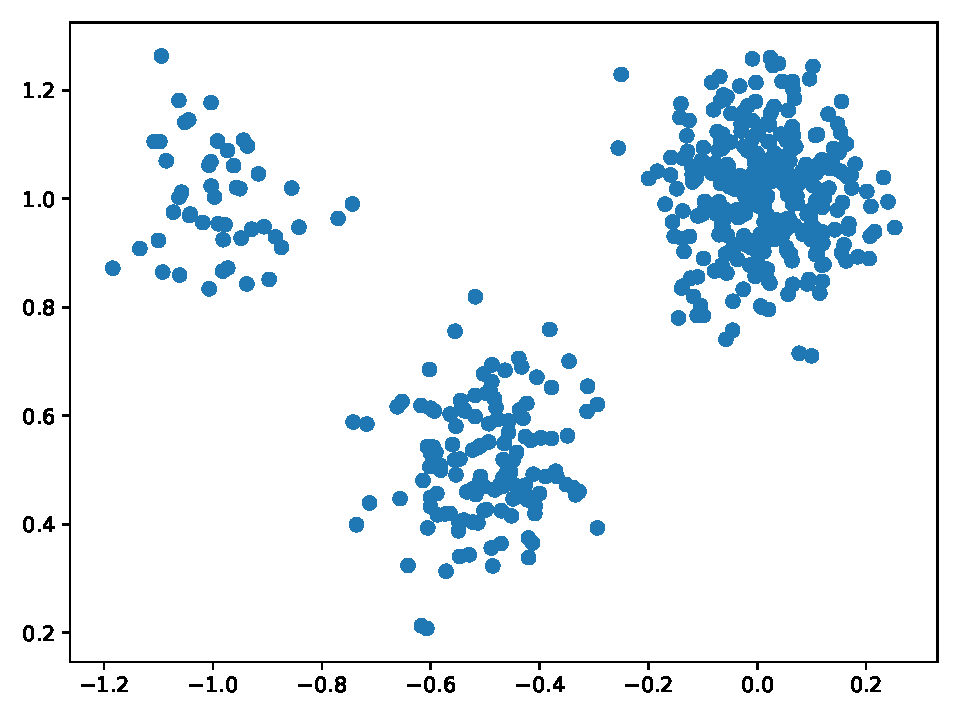
\includegraphics{images/gmm.pdf}
	\caption{$500$ realizations of a Gaussian mixture with $d=2$, $K=3$ and the following parameters $\pi = [\pi_1, \pi_2, \pi_3] = [0.1, 0.6, 0.3]$, $\mu_1 = [-1, 1]$, $\mu_2 = [0, 1]$, $\mu_3 = [-0.5, 0.5]$ and $\bSigma_1 = \bSigma_2 = \bSigma_3 = 0.01 \times \bI_2$.}
\end{marginfigure}
for any $x \in \R^d$, where $\theta = (\pi_k, \mu_k, \bSigma_k)_{k=1, \ldots, K}$ and $K \geq 1$ is an integer corresponding to the number of ``clusters''.
Such a mixture density is non-identifiable, since we have $f_{\theta} = f_{\sigma(\theta)}$
for any permutation $\sigma(\theta) = (\pi_{\sigma(k)}, \mu_{\sigma(k)}, \bSigma_{\sigma(k)})_{k=1, \ldots, K}$ of $\theta$ where $\sigma$ is a permutation of $\{1, \ldots, K \}$.
This simply means that the density distribution $f_\theta$ is invariant by a relabeling of the clusters numbers.
Despite the fact that such a mixture model is not identifiable, it is often used for \emph{model-based clustering}, which is an instance of \emph{unsupervised learning}.
Another family of non-identifiable models is deep neural networks, in which an infinitely large number of parametrizations lead to the same prediction function.

\section{Dominated models} 

Whenever $\cP = \{ P_\theta : \theta \in \Theta \}$ with $\Theta \subset \R^d$, we say that $\cP$ is a \emph{parametric} model, since it is parametrized by a finite-dimensional parameter, trivial instances being $\{ \ber(\theta) : \theta \in (0, 1) \}$ for which $d=1$ and $\{ \nor(\mu, v) : (\mu, v) \in \R \times (0, +\infty) \}$ for which $d=2$.
We say that both models are \emph{dominated}, the first being dominated by the counting measure $\nu = \delta_0 + \delta_1$ on $\{ 0, 1\}$,%
\sidenote{The notation $\delta_x$ will stand for the Dirac mass at $x$ which is the probability measure satisfying $\int f(u) \delta_x(du) = f(x)$ for any measurable function $f$.}%
and the second by the Lebesgue measure on $\R$.\sidenote{We recall that if $P$ and $Q$ are two measures on the same probability space, $P \ll Q$ means that the measure $P$ is \emph{absolutely continuous} with respect to $Q$, namely that $Q(A) = 0 \Rightarrow P(A)= 0$ for any measurable set $A$.}
\begin{definition}
	\label{def:dominated-model}
	We say that a model $\cP = \{ P_\theta : \theta \in \Theta \}$ is dominated if there is a $\sigma$-finite measure $\mu$ such that $P_\theta \ll \mu$ for all $\theta \in \Theta$.
\end{definition}
In Definition~\ref{def:dominated-model}, we require that the dominating measure is $\sigma$-finite, so that we can apply the Radon-Nikodym theorem: since $P_\theta \ll \mu$ for all $\theta \in \Theta$, there is a density 
\begin{equation*}
	f_\theta = \frac{dP_\theta}{d\mu}
\end{equation*}
for all $\theta \in \Theta$.
This domination property allows to work with densities instead of distributions: a model can be therefore defined as a family of densities $\{ f_\theta : \theta \in \Theta \}$ together with a dominating measure (which is in most cases the Lebesgue measure, a counting measure, or a combination of them.)
\begin{example}
	Let us consider the \emph{zero-inflated Laplace distribution}, which is a distribution on $\R$ given by
	\begin{equation*}
		P_\theta(dx) = \pi_0 \delta_0(dx) + (1 - \pi_0) \frac{\lambda}{2} e^{-\lambda |x|} dx
	\end{equation*}
	for $\theta = (\pi_0, \lambda) \in \Theta = (0, 1) \times (0, +\infty)$, which is dominated by the measure $\mu = \delta_0 + \leb$, where $\leb$ stands from now on for the Lebesgue measure on $\R$.
\end{example}
Non-dominated models are usually pathological and uninteresting examples, such as the model
\begin{equation*}
	P_\lambda = \frac 1e \sum_{n \geq 0} \frac{1}{n!} \delta_{\lambda n}
\end{equation*}
for $\lambda \in (0, +\infty)$, which cannot be dominated by a $\sigma$-finite measure.

Let us finish this chapter with an example of non-parametric model: we observe $X_1, \ldots, X_n$ with a density $f \in F$ with respect to the Lebesgue measure, where $F$ is the set of probability densities on $[0, 1]^d$ that are $C^2$ and such that $\grad^2 f(x) \mleq L \bI_d$.%
\sidenote{The notation $\nabla^2 f(x)$ stands for the Hessian matrix of $f$, while $\bI_d$ is the identity matrix on $\R^d$. Finally, for two symmetric matrices $\bA$ and $\bB$, the notation $\bA \mleq \bB$ means $\bB - \bA \mgeq 0$, namely that $\bB - \bA$ is a symmetric and positive semi-definite matrix.}%
In such a setting, we work with an infinite dimensional set of parameters $F$, and need to build a \emph{non-parametric} estimator of the unknown density $f$.



\setchapterpreamble[u]{\margintoc}
\chapter{Statistical inference}
\label{chap:statistical_inference}

In this Chapter, we will consider all along the simple Bernoulli model, where we have iid samples $X_1, \ldots, X_n$ distributed as $\ber(\theta)$ with $\theta \in (0, 1)$.
Let us start with the first \emph{inference} problem: the \emph{estimation} problem.

\section{Estimation} % (fold)
\label{sec:estimation}

We want to \emph{infer} $\theta$, or \emph{estimate} it by finding a statistic which is a measurable function of $(X_1, \ldots, X_n)$%
\sidenote{Once again, since we are doing statistics, the only thing we are allowed to use is the data.}%
or a measurable function of $S_n = \sum_{i=1}^n X_i$ thereof, since $S_n$ is sufficient, see Section~\ref{sec:statistics}.
We will denote such a statistic as
\begin{equation*}
 	\wh \theta_n = \wh \theta(X_1, \ldots, X_n).
\end{equation*}
This function \emph{does not depend} on $\theta$, but its distribution does.
Ideally, we want $\wh \theta_n$ to be ``close'' to $\theta$, since we want a good estimator, so that the first thing we need to do is to quantify ``closeness''.
For instance, we could want $|\wh \theta_n - \theta|$ to be close to $0$ with a large probability, since we do not forget that $\wh \theta_n$ is a random variable, as a function of the data $(X_1, \ldots, X_n)$.
The most natural distance is arguably the Euclidean one, in this context the $L^2$ distance, 
which leads to the \emph{quadratic risk}.%
\sidenote{Although the quadratic risk corresponds to a \emph{squared} $L^2$ norm.}
\begin{definition}[Quadratic risk]
	\label{def:quadratic_risk}
	Consider a statistical model with data $X$ and set of parameters $\Theta \subset \R$ and an estimator $\wh \theta(X)$. 
	The quadratic risk of $\wh \theta$ is given by
	\begin{equation*}
		R(\wh \theta, \theta) = \E_\theta[ (\wh \theta - \theta)^2 ] = \int_E (\wh \theta(x) - \theta)^2 P_\theta(dx).
	\end{equation*}
	We consider the quadratic risk as a function $\Theta \goes \R^+$ of the parameter given by $\theta \mapsto R(\wh \theta, \theta)$.
\end{definition}
At this point, it's useful to recall some classical inequalities on the queues of random variables.
The Markov inequality tells us that if $Y$ is a real random variable such that $\E |Y|^p < +\infty$ for some $p > 0$ then
\begin{equation*}
	\P(|Y| > t) \leq \frac{\E |Y|^p}{t^p}
\end{equation*}
for any $t > 0$.
This tells us that the more $Y$ has moments%
\sidenote{We say that $Y$ as moments up to order $p$ if $\E |Y|^p < +\infty$. 
Note that this entails $\E |Y|^q < +\infty$ for any $q < p$ since $\E |Y|^p = \E (|Y|^q)^{p/q} \geq (\E |Y|^q)^{p/q}$ using Jensen's inequality.}%
the more the queue of $Y$ is tight (it goes faster to $0$ with $t \goes +\infty$).
Markov's inequality with $p=2$ entails 
\begin{equation}
	\label{eq:l2_entrails_proba}
	\P(|\wh \theta - \theta| > t) \leq \frac{R(\wh \theta, \theta)}{t^2}
\end{equation}
which tells us that whenever the quadratic risk is small, then $\wh \theta$ is close to $\theta$ with a large probability.

Whenever $R(\wh \theta_n, \theta) \rightarrow 0$ with $n \rightarrow +\infty$, we will write $\wh \theta_n \goqr \theta$, which stands for convergence in $L^2$ norm, which entails, because of Inequality~\eqref{eq:l2_entrails_proba}, that $\wh \theta_n \gopro \theta$, which stands for convergence in probability.\sidenote{More precisely, in $\P_\theta$-probability, namely $\P_\theta[|\wh \theta_n - \theta| > \eps] \rightarrow 0$ as $n \rightarrow +\infty$ for any $\eps > 0$, but we will write $\wh \theta_n \gopro \theta$ in order to keep the notations as simple as possible.}%
\begin{definition}
	\label{def:consistent}
	We say that $\wh \theta_n$ is \emph{consistent} whenever $\P_\theta[|\wh \theta_n - \theta| > \eps] \rightarrow 0$ as $n \rightarrow +\infty$ for any $\eps > 0$ and any $\theta \in \Theta$.
	We say that it is strongly consistent whenever $\P_\theta[\wh \theta_n \rightarrow \theta] = 1$ for any $\theta \in \Theta$.
\end{definition}
In Definitions~\ref{def:quadratic_risk} and~\ref{def:consistent} above, if $\Theta \subset \R^d$, it suffices to replace $|\cdot|$ by the Euclidean norm $\norm{\cdot}_2$.%
\sidenote{We can use any norm on $\R^d$ in Definition~\ref{def:consistent}, and let us recall that $\norm{x}_2 = \sqrt{x^\top x} = (\sum_{j=1}^d x_j^2)^{1/2}$.}%

\paragraph{Bias variance decomposition.} % (fold)

The \emph{bias-variance decomposition} is the following decomposition of the quadratic risk between two terms: a bias term denoted $b(\wh \theta_n, \theta)$ (squared in the formula) and a variance term:
\begin{equation}
	\label{eq:bias-variance-decomposition}
	\begin{split}
	R(\wh \theta_n, \theta) &= \E_\theta[(\wh \theta_n - \theta)^2] = (\E_\theta \wh \theta_n - \theta)^2 + \var_\theta(\wh \theta_n) \\
	&= b(\wh \theta_n, \theta)^2 + \var_\theta(\wh \theta_n).		
	\end{split}
\end{equation}
When $b(\wh \theta_n, \theta) = 0$ for all $\theta \in \Theta$ we say that the estimator $\wh \theta_n$ is \emph{unbiased}.
This means that this estimator will not tend to over or under-estimate $\theta$. 

\paragraph{Back to Bernoulli.} % (fold)

% paragraph back_to_bernoulli (end)Back to Bernoulli
Going back to the $\ber(\theta)$ model, we consider the estimator $\wh \theta_n = S / n = \sum_{i=1}^n X_i / n$.
We already know many things about this estimator:
\begin{enumerate}
	\item We have $\E_\theta [\wh \theta_n] = \theta$ which means that $\wh \theta_n$ is unbiased;
	\item The bias-variance decomposition gives
	\begin{equation}
		\label{eq:bernoulli-quadratic-risk}
	 	R(\wh \theta_n, \theta) = \var(\wh \theta_n) = \frac{\theta (1 - \theta)}{n} \leq 
	 	\frac{1}{4 n} \rightarrow 0
	 \end{equation}
	 which means that $\wh \theta_n \goqr \theta$ and which entails that $\wh \theta_n$ it is consistent;
	\item The law of large number tells us that $\wh \theta_n \goas \theta$, hence $\wh \theta_n$ is strongly consistent;
	\item The central limit theorem tells us that
	\begin{equation}
	\label{eq:tcl-bernoulli}
	\sqrt n (\wh \theta_n - \theta) \leadsto \nor(0, \theta(1 - \theta)).
	\end{equation}
\end{enumerate}
The points 2--4 from above are all different ways of saying that when $n$ is large enough, then $\wh \theta_n$ is close to $\theta$.
In practice, an estimator leads to a value: for the Bernoulli model with $n=100$ and $42$ ones you end up with a single estimated value $0.42$.
But what if we want to include uncertainty in this estimation ?
Namely how confident are we about this $0.42$ value ?
Moreover, what do we mean by ``when $n$ large enough'', can we quantify this better ?
All these questions can be answered by considering another inference problem: confidence intervals.

\section{Confidence intervals} % (fold)
\label{sec:confidence_intervals}

Here, we don't only want to build an estimator $\wh \theta_n$ but also to quantify the uncertainty of this estimation.
Combining Inequalities~\eqref{eq:l2_entrails_proba} and~\eqref{eq:bernoulli-quadratic-risk} leads to
\begin{equation*}
	\P_\theta[ |\wh \theta_n - \theta| > t] \leq \frac{1}{4 n t^2}
\end{equation*}
so that for $\alpha \in (0, 1)$ and the choice $t_\alpha = 1 / (2 \sqrt{n \alpha})$ we have 
\begin{equation*}
	\P_\theta \{ \theta \in [ \wh \theta^L, \wh \theta^R ] \} \geq 1 - \alpha,
\end{equation*}
where
\begin{equation*}
	\wh \theta^L =  \wh \theta_n - \frac{1}{2 \sqrt{n \alpha}} \quad \text{ and } \quad \wh \theta^R =  \wh \theta_n + \frac{1}{2 \sqrt{n \alpha}}.
\end{equation*}
Therefore, if we choose $\alpha = 0.05 = 5\%$, we know that $\theta \in [\wh \theta^L, \wh \theta^R]$ with a probability larger than $95\%$.
We say in this case that the interval $[\wh \theta^L, \wh \theta^R]$ is a \emph{confidence interval} with coverage $95\%$.%
\sidenote{If we toss the coin $1000$ times and get $420$ heads, the realization of this confidence interval at $95\%$ is $[0.35, 0.49]$.}

Note that if $\alpha = 0$ then we have no other choice than using the whole $\R$ as a confidence interval: $\alpha$ allows to give some slack, so that we can build a non-absurdly  large confidence interval. 
We typically have that $|\wh \theta^R - \wh \theta^L|$ increases as $\alpha$ decreases, since a smaller $\alpha$ means more confidence, hence a larger interval.
On the contrary, $|\wh \theta^R - \wh \theta^L|$ should decrease with the sample size $n$.
\begin{definition}[Confidence interval]
	Consider a statistical model with data $X$ and set of parameters $\Theta \subset \R$. 
	Fix a \emph{confidence level} $\alpha \in (0, 1)$ and consider two statistics $\wh \theta^L(X)$ and $\wh \theta^R(X)$. Whenever 
	\begin{equation}
		\label{eq:coverage-property}
		\P_\theta\{ \theta \in [\wh \theta^L(X), \wh \theta^R(X)] \} \geq 1 - \alpha
	\end{equation}
	for any $\theta \in \Theta$, we say that $[\wh \theta^L(X), \wh \theta^R(X)]$ is a \emph{confidence interval} at level $1 - \alpha$.
\end{definition}
Inequality~\eqref{eq:coverage-property} is called the \emph{coverage} property of the confidence interval.
More generally, when $\Theta \subset \R^d$, we will say that $S(X)$ is a \emph{confidence set} if it is a statistic satisfying the coverage property $\P_\theta\{ \theta \in S(X) \} \geq 1 - \alpha$ for any $\theta \in \Theta$.
\begin{remark}
	Whenever we need only an upper or lower bound on $\theta$ (for instance, when we need to check statistically that some toxicity level is below some threshold), we build a \emph{unilateral} or \emph{one-sided} confidence interval, where we choose either $\wh \theta^L = -\infty$ ($0$ for the Bernoulli model) or $\wh \theta^R = +\infty$ ($1$ for the Bernoulli model).
	Indeed, at a fixed level $1 - \alpha$, the bound of a one-sided confidence interval is tighter than the same sided bound corresponding to a two-sided interval. 
\end{remark}
But, we can do better for the Bernoulli model (or any model where $X$ is bounded) thanks to the following Hoeffding inequality.
\begin{theorem}
	\label{thm:hoeffding}
	Let $X_1, \ldots, X_n$ be independent random variables such that $X_i \in [a_i, b_i]$ almost surely and let $S = \sum_{i=1}^n X_i$. Then,
	\begin{equation*}
		\P[ S \geq \E S + t] \leq \exp\Big( - \frac{2 t^2}{\sum_{i=1}^n (b_i - a_i)^2} \Big)
	\end{equation*}
	holds for any $t >0$.
\end{theorem}
Theorem~\ref{thm:hoeffding} is something called a deviation inequality: it provides a control on the probability of deviation of $S$ with respect to its mean.
It shows that bounded random variables are \emph{sub-Gaussian}, since it shows that the queue of $S - \E S$ is bounded by $\exp(-c t^2)$ for some constant $c$ (that depends on $n$).
The proof of this inequality is provided in Chapter~??\todo{insert reference} below.
\todo{Provide the proof of Hoeffding}

\paragraph{Back to Bernoulli.} % (fold)

% paragraph back_to_bernoulli (end)
Let's apply Theorem~\ref{thm:hoeffding} to the Bernoulli model $X_i \sim \ber(\theta)$ so that $a_i = 0$, $b_i = 1$ and therefore $\P[ S \geq \E S + t] \leq e^{-2 t^2 / n}$.
Using again Theorem~\ref{thm:hoeffding} with $X_i$ replaced by $-X_i$ together with an union bound%
\sidenote{}%
leads to $\P[ | S - \E S | \geq t] \leq 2 e^{-2 t^2 / n}$.
So, for some $\alpha \in (0, 1)$, we obtain another confidence interval, since the following coverage property holds:
\begin{equation*}
	\P \bigg[ \wh \theta_n - \sqrt{\frac{\log(2 / \alpha)}{2n}} \leq \theta \leq \wh \theta_n 
	+ \sqrt{\frac{\log(2 / \alpha)}{2n}} \bigg] \geq 1 - \alpha.
\end{equation*}
This proves that $[\wh \theta \pm \sqrt{\log(2 / \alpha) / (2n)}]$ is a confidence interval at level $1 - \alpha$.%
\sidenote{For $1000$ tosses and $420$ heads, the realization of this interval at level $95\%$ is $[0.37, 0.46]$. It's a bit more precise than the previous one, which was based on Markov's inequality.}
Let's compare the two confidence intervals we obtained so far for the Bernoulli model.
We have of course
\begin{equation*}
	\frac{1}{2 \sqrt{n \alpha}} > \sqrt{\frac{\log(2 / \alpha)}{2n}} 
\end{equation*}
for $\alpha$ small enough\todo{etre plus precis ici}, although both sides are $O(1 / \sqrt n)$.
Only the dependence on the level $\alpha$ is improved with the confidence interval obtained through Hoeffding's inequality, since it exploits the sub-Gaussianity of the Bernoulli distribution, while the first confidence interval only used the upper bound~\eqref{eq:l2_entrails_proba} on the variance.%
\sidenote{There is yet another way to build a (non-asymptotic) confidence interval, using a more computational approach, see for instance ????}

\paragraph{Asymptotic coverage.}

For both the previous confidence intervals, we adopted a \emph{non-asymtotic} approach: the coverage properties hold for any value of $n \geq 1$.
This is possible since we know things about the distribution of $S$, which is a simple $\bin(n, \theta)$ distribution.
However, in general, the \emph{exact} distribution of an estimator $\wh \theta_n$ cannot always be made explicit, and in such cases, we often use Gaussian approximations, thanks to the central limit theorem. 
Let's do this for the Bernoulli model.
Indeed, we know from~\eqref{eq:tcl-bernoulli} that
\begin{equation}
	\label{eq:portemanteau-bernoulli}
	\P_\theta \bigg[ \sqrt{\frac{n}{\theta (1 - \theta)}} (\wh \theta_n - \theta) \in I
	\bigg] \rightarrow \P[Z \in I]
\end{equation}
where $Z \sim \nor(0, 1)$ for any closed interval $I \subset \R$.%
\sidenote{This uses the porte-manteau theorem, which says that $X_n \gosto X$ if and only if $\P(X_n \in A) \goes \P(X \in A)$ for any Borelian set $A$ such that $\P(X \in \partial A) = 0$, where $\partial A$ stands for the boundary of $A$.}%
Using $I = [-q_\alpha, q_\alpha]$ with $q_\alpha = \Phi^{-1}(1 - \alpha / 2)$ we end up%
\sidenote{We recall that $\Phi^{-1}$ is the inverse of the distribution function $\Phi(x) = \P( Z \leq x)$ of the $\nor(0, 1)$ distribution, that we call the \emph{quantile} function of $\nor(0, 1)$.}%
with the fact that
\begin{equation}
	\label{eq:not-and-ic}
	\P_\theta\bigg\{ \theta \in \Big[ \wh \theta_n \pm q_\alpha \sqrt{\frac{\theta(1 - \theta)}{n}} \Big] \bigg\} \rightarrow 1 - \alpha.
\end{equation}
This is interesting, but not enough to build a confidence interval, since the interval in Equation~\eqref{eq:not-and-ic} depends on $\theta$ through the variance term $\theta(1 - \theta)$.
Indeed, a confidence interval must be something that does \emph{not} depend on $\theta$.
We need to work a little bit more in order to remove the dependence on $\theta$ from this interval. 
We do the same as before: we use the fact that $\theta (1 - \theta) \leq 1 / 4$ for any $\theta \in [0, 1]$, so that
\begin{equation*}
	\liminf_n \P_\theta \bigg\{ \theta \in \Big [\wh \theta_n \pm \frac{q_\alpha}{2 \sqrt n} \Big] \bigg\} \geq 1 - \alpha.
\end{equation*}
This is what we call a confidence interval \emph{asymptotically of level} $1 - \alpha$ constructed \emph{by excess}.

In the above construction of an asymptotic confidence interval, we used the central limit theorem to approximate the $\bin(n, \theta)$ distribution (the distribution of $S = \sum_{i=1}^n X_i$) by a Gaussian distribution.
This requires $n$ to be ``large enough'', but the central limit theorem does not tell us how large.
We can quantify this better by trying to quantify how close the distribution function of $S$ is to the one of $\nor(0, 1)$, using the following theorem.
\begin{theorem}[Berry-Esseen]
	Let $X_1, \ldots, X_n$ be i.i.d random variables such that $\E X_i = 0$ and $\var(X_i) = \sigma^2$ and introduce the distribution function%
	\marginnote{BLABLABLA}%
	\begin{equation*}
		F_n(x) = \P \bigg[ \frac{\sum_{i=1}^n X_i}{\sqrt{n \sigma^2}} \leq x \bigg]
	\end{equation*}
	for any $x \in \R$. Then, the following inequality holds:
	\begin{equation*}
		\sup_{x \in \R} |F_n(x) - \Phi(x)| \leq \frac{c \kappa}{\sigma^3 \sqrt n},
	\end{equation*}
	where $\kappa = \E |X_1|^3$ (assumed finite) and where $c$ is a purely numerical constant (the best known one is $c = 0.4748$).
\end{theorem}
We provide a proof with a worse constant $c$ in Section~??? below.\todo{insert proof}
Note that there is also a lower bound with $c \geq 0.4097$, as explained in ?? and that the best constant $c = 0.4748$ for the upper bound is from ???.
Note also that a similar result holds if the $X_i$ are independent but not identically distributed.

For Bernoulli with have $\E|X_1|^3 = \theta$ and $\sigma^3 = (\theta(1 - \theta))^{3/2}$ so that 
\begin{equation*}
	|F_n(x) - \Phi(x)| \leq \frac{3}{\sqrt{n \theta (1 - \theta)^3}}
\end{equation*}
which shows that the approximation by the Gaussian distribution deteriorates whenever $\theta$ is close to $0$ or $1$.

\paragraph{Reparametrization.} % (fold)

Another asymptotic approach allowing to get rid of the dependence on $\theta$ in the confidence interval~\eqref{eq:not-and-ic} is based on the idea of reparametrization.
Indeed, given a statistical model $\{ P_\theta : \theta \in \Theta \}$ and a bijective function $g : \Theta \goes \Lambda$ we can use instead the ``reparametrized''model $\{ Q_\lambda : \lambda \in \Lambda \}$ where $Q_\lambda = P_{g^{-1}(\lambda)}$.
Let us also remark that if $[\wh \theta^L, \wh \theta^R]$ is a confidence interval for $\theta$ at level $1 - \alpha$ and if $g$ is an increasing function, then 
$[g(\wh \theta^L), g(\wh \theta^R]$ is a confidence interval for $g(\theta)$ at level $1 - \alpha$.
Now, a natural question is to understand if the convergences we used above (in particular, the convergence in distribution involved in the central limit theorem) is stable under such a reparametrization.
\begin{example}
	\label{ex:expo}
	Consider a iid dataset $X_1, \ldots, X_n$ with distribution $\expo(\theta)$ with scale parameter $\theta > 0$, namely the distribution $P_\theta(dx) = \theta e^{-\theta x} \ind{x \geq 0} dx$. 
	We have $\E(X_1) = 1 / \theta$ and $\var(X_1) = 1 / \theta^2$, so that using the law of large numbers and the central limit theorem we have
	\begin{equation*}
		\bar X_n \goas \theta^{-1} \quad \text{ and } \quad \sqrt n (\bar X_n - \theta^{-1}) \leadsto \nor(0, \theta^{-2})
	\end{equation*}
	when $n \rightarrow +\infty$.
	Since $x \mapsto 1 / x$ is a continuous function on $(0, +\infty)$, we know that $(\bar X_n)^{-1} \goas \theta$ so that a strongly consistent estimator is given by $\wh \theta = (\bar X_n)^{-1}$.
	But what can we say about the convergence in distribution of 
	$\sqrt n (\wh \theta_n - \theta)$ ?
\end{example}
This is answered by so-called $\Delta$-method, described in the next theorem.
\begin{theorem}[$\Delta$-method]
	\label{thm:delta-method}
 	Let $(Z_n)_{n \geq 1}$ be a sequence of real random variables and assume that 
	$a_n(Z_n - z) \leadsto Z$, where $(a_n)_{n \geq 1}$ is a positive sequence such that $a_n \goes +\infty$, where $z \in \R$ and where $Z$ is a real random variable.
 	If $g$ is a function defined on a neighborhood of $z$ and differentiable at $z$, we have 
 	\begin{equation}
 		a_n (g(Z_n) - g(z)) \leadsto g'(z) Z
 	\end{equation}
 	as $n \goes +\infty$.
\end{theorem}
The proof easily follows from a first-order Taylor expansion of $g$ around~$z$, as explained in Section~??? below. \todo{insert proof}
A particularly useful case for statistics is when $Z$ is Gaussian.
For instance, if $\sqrt n (\wh \theta_n - \theta) \leadsto \nor(0, \sigma(\theta)^2)$, we have
\begin{equation*}
	\sqrt n (g(\wh \theta_n) - g(\theta)) \leadsto 
	\nor(0, \sigma(\theta)^2 (g'(\theta))^2)
\end{equation*}
whenever $g$ satisfies the conditions of Theorem~\ref{thm:delta-method}.
Going back to the $\expo(\theta)$ example from Example~\ref{ex:expo}, we obtain with $g(x) = 1 / x$ and since $\wh \theta = g(\bar X_n)$ that $\sqrt n (\wh \theta - \theta) \leadsto \nor(0, \theta^2)$.
Another result which provides stability for the convergence in distribution under a smooth mapping is the so-called Slutsky theorem.
\begin{theorem}[Slutsky]
	\label{thm:slutsky}
	Let $(X_n)_{n \geq 1}$ and $(Y_n)_{n \geq 1}$ be sequences of real random variables such that $X_n \leadsto X$ and $Y_n \leadsto y$ where $X$ is some real random variable and $y \in \R$.
	Then, we have that $Y_n \gopro y$ and $(X_n, Y_n) \leadsto (X, y)$ as $n \goes +\infty$. In particular, we have $f(X_n, Y_n) \leadsto f(X, y)$ for any continuous function $f$.
\end{theorem}
The proof of Theorem~\ref{thm:slutsky} is given in Section~? below.\todo{insert proof}
The $\Delta$-method provides stability for the convergence in distribution when a differentiable function is applied to a sequence, while Slutsky theorem provides ``algebraic'' stability when combining two sequences converging respectively in distribution and probability.
\sidenote{Be careful with convergence in distribution. Please keep in mind that this mode of convergence is about the convergence of the distributions and not the convergence of the random variables (hence its name). The notation $X_n \gosto X$ is rather misleading but convenient. In particular, nothing can be said in general about $f(X_n, Y_n)$ when we know that $X_n \gosto X$ and $Y_n \gosto Y$ (unless $X_n$ and $X_n$ are independent sequences).}

\paragraph{Back again to Bernoulli.}

We have $\wh \theta_n \gopro \theta$, so that $(\wh \theta_n (1 - \wh \theta_n)^{1/2} \gopro (\theta (1 -  \theta))^{1/2}$ since $x \mapsto (x(1-x))^{1/2}$ is continuous on $[0, 1]$ and let us write
\begin{equation*}
	\frac{\sqrt n (\wh \theta_n - \theta)}{\sqrt{\wh \theta_n (1 - \wh \theta_n)}} 
	= \frac{\sqrt n (\wh \theta_n - \theta)}{\sqrt{ \theta (1 -  \theta)}} \times 
	\sqrt{\frac{ \theta (1 -  \theta)}{\wh \theta_n (1 - \wh \theta_n)}} =: A_n \times B_n.
\end{equation*}
We know that $A_n \gosto \nor(0, 1)$ and that $B_n \gopro 1$.
Therefore, using Theorem~\ref{thm:slutsky} leads%
\sidenote{With $f(x, y) = xy$.}%
to
\begin{equation*}
	\sqrt{\frac{n}{\wh \theta_n (1 - \wh \theta_n)}} (\wh \theta_n - \theta) \gosto \nor(0, 1).
\end{equation*}
Yes, we just replaced $\theta$ by $\wh \theta_n$ in the variance term $\theta(1 - \theta)$ of the limit~\eqref{eq:portemanteau-bernoulli}, but doing so required Slutsky's theorem to prove this rigorously, and this provides us another confidence interval with asymptotic coverage given by
\begin{equation*}
	\P_\theta \bigg\{ \theta \in \Big[ \wh \theta_n \pm q_\alpha \sqrt{\frac{\wh \theta_n (1 - \wh \theta_n)}{n}} \Big] \bigg\} \goes 1 - \alpha
\end{equation*}
as $n \goes +\infty$.%
\sidenote{With $1000$ tosses and $420$ heads, the realization of this confidence interval at level $95\%$ is $[0.38, 0.45]$.}%


\section{Tests} % (fold)
\label{sec:tests}

Let us consider, again, in this section, a statistical experiment with data $X$ and model $\{ P_\theta : \theta \in \Theta \}$.
Here, we want to decide between to hypothesis $H_0$ and $H_1$, where
\begin{equation*}
	H_i \quad \text{means that} \quad \theta \in \Theta_i
\end{equation*}
for $i \in \{ 0, 1 \}$, where $\{ \Theta_0, \Theta_1 \}$ is a partition of the set of parameters~$\Theta$.
In order to understand the concept of statistical testing, let us consider the following unsettling example: imagine that you need to decide if a patient has cancer or not.
The patient has cancer if some parameter $\theta \in (0, 1)$ about him satisfies
$\theta \geq 0.42$.
We \emph{choose} $\Theta_0 = [0.42, 1]$ and $\Theta_1 = [0, 0.42)$, namely we decide that $H_0$ means that the patient has cancer, while $H_1$ means that the patient has not.
We need to construct a testing function $\varphi : E \goes \{ 0, 1 \}$ that maps $X \mapsto \varphi(X)$, our decision being given by the value of $\varphi(X)$. 
We decide that $H_0$ is true whenever $\varphi(X) = 0$, in this case we say that we \emph{accept} $H_0$ and we \emph{reject} $H_0$ whenever $\varphi(X) = 1$.
This is a convention, the $1$ in $\varphi(X) = 1$ and $H_1$ will always mean that we \emph{reject} the \emph{null hypothesis} $H_0$.

\paragraph{Type I and Type II errors.}

When $\theta \in \Theta_i$, we are correct if $\varphi(X) = i$ and incorrect if $\varphi(X) = 1 - i$.
We have two types of errors: the \emph{Type-I error}, also called the \emph{first-order error}, given by 
\begin{equation}
	\label{eq:type-1-error}
	\P_\theta[ \varphi(X) = 1] = \E_\theta [\varphi(X)] \quad \text{for} \quad
	\theta \in \Theta_0
\end{equation}
and the \emph{Type-II error}, also called \emph{second-order error}, given by 
\begin{equation}
	\label{eq:type-2-error}
	\P_\theta[ \varphi(X) = 0] = 1 - \E_\theta [\varphi(X)] \quad \text{for} \quad 
	\theta \in \Theta_1.
\end{equation}
For the cancer detection problem, the Type~I error corresponds to the \emph{probability of saying to the patient that he has not cancer while he has.}
The Type~II error corresponds to the \emph{probability of saying to the patient that he has cancer while he has not}.
Note that these two types of errors are not symmetrical: we consider that the first one is more serious than the second (although this can be debated, the patient could do a depression, or start an invasive treatment for nothing).%
\sidenote{Of course this morbid example is highly unrealistic, and is used only to stress the asymmetry of errors in a statistical testing problem.}
The important point here is that $H_0$ and $H_1$ must be \emph{chosen} depending on the practical application considered. 
They are not \emph{given} and they correspond to an important modeling choice.
We will see below that $H_0$ and $H_1$ must be chosen, in practice, so that the corresponding Type I error is \emph{more serious}, for the considered application, than the Type II error.
\begin{definition}
	\label{def:power-function}
	The function $\beta : \Theta \goes [0, 1]$ that maps $\theta \mapsto \beta(\theta) = \E_\theta [\varphi(X)]$ is called the \emph{power function} of the test $\varphi$.
\end{definition}
Ideally, we would like both the Type~I and Type~II errors to be small, namely $\beta(\theta) \approx 0$ for $\theta \in \Theta_0$ and $\beta(\theta) \approx 1$ for $\theta \in \Theta_1$.
But this is impossible: if $\Theta$ is a connected set then $\Theta_0$ and $\Theta_1$ share a common frontier, so that $\beta$ must be discontinuous on it, while $\beta$ is in general a continuous function.\todo{donner sa valeur dans le cas bernoulli}
Therefore, it is hard to make both the Type~I and Type~II errors small at the same time.

\todo{en fait faudrait donner l'exemple du cancer ici... ?}

\paragraph{Desymmetrization of statistical tests.} % (fold)

The way a statistical test is performed is through the \emph{Neyman-Pearson approach}, where we  \emph{desymmetrize} the problem: choose the hypothesis $H_0$ using common sense, so that the hypothesis leading to a Type~I error that is more serious than the Type~II error.
The Type~I error is always the rejection of $H_0$ when it is true, while the Type~II error is always the acceptation of $H_0$ when it is false.
The only thing that we choose is what are $H_0$ and $H_1$.
Let us wrap up all what we said before, and introduce some extra things.
\begin{definition}
	\label{def:test-definitions}
	Consider a statistical testing problem with hypothesis
	\begin{equation*}
		H_0 : \theta \in \Theta_0 \quad \text{versus} \quad H_1 : \theta \in \Theta_1
	\end{equation*}
	and a testing function $\varphi : E \goes \{ 0, 1 \}$.
	We call $H_0$ the \emph{null} hypothesis and $H_1$ the \emph{alternative} hypothesis.
	When $\varphi(X) = 0$ we say that the test \emph{accepts} $H_0$ or simply that it \emph{accepts}. When $\varphi(X) = 1$ the test \emph{rejects}.
	\begin{enumerate}
		\item The set $R = \{ x \in E : \varphi(x) = 1 \}$ is called the \emph{rejection set} or the \emph{rejection region} of the test $\varphi$, and we call $R^\complement$ the \emph{acceptation region};
		% \item The function $\beta : \Theta \goes [0, 1]$ given by $\beta(\theta) = \E_\theta [\varphi(X)]$ is called the \emph{power function} of the test;
		\item The restriction of the power function $\beta$ from Definition~\ref{def:power-function} $\beta : \Theta_0 \goes [0, 1]$ is called the \emph{Type~I error}, while the restriction $\beta : \Theta_1 \goes [0, 1]$ is called the \emph{power} of the test. The function $1 - \beta : \Theta_1 \goes [0, 1]$ is called the \emph{Type~II error} or \emph{second order error}.
		\item Whenever $\sup_{\theta \in \Theta_0} \beta(\theta) \leq \alpha$ for some fixed $\alpha \in (0, 1)$, we say that the test \emph{has level} $\alpha$.
	\end{enumerate}
\end{definition}
The idea of desymmetrization is as follows: given a level $\alpha \in (0, 1)$ (something like $1\%$, $5\%$ or $10\%$) we build a test so that it has, \emph{by construction}, level $\alpha$.
Namelu, a test is \emph{built so that the Type~I error is controlled}, while nothing is done directly about the Type~II error.
Given two statistical tests with level $\alpha$ (namely Type~I error $\leq \alpha$), we can simply compare their Type~II error and choose the one that maximizes it.

\paragraph{Back to Bernoulli.} % (fold)

Let us go back to the Bernoulli model where $X_1, \ldots, X_n$ are iid and distributed as $\ber(\theta)$.
We consider the problem of statistical testing with hypothesis:
\begin{equation}
	\label{eq:chap03-tests-hypothesis}
	H_0 : \theta \leq \theta_0 \quad \text{ against } \quad H_1 : \theta > \theta_0
\end{equation}
so that $\Theta = (0, 1)$ and $\Theta_0 = (0, \theta_0]$ and $\Theta_1 = (\theta_0, 1)$.
We studied in Sections~\ref{sec:estimation} and~\ref{sec:confidence_intervals} the estimator $\wh \theta_n = \bar X_n$, and know that it is a good estimator.
A natural idea is therefore to reject $H_0$ if $\wh \theta_n$ is too large.
\begin{recipe}
	We build a test by defining its rejection set $R$. The shape of the rejection set can be easily guessed by looking at the alternative hypothesis $H_1$.
\end{recipe}
Since we want to reject when $\theta > \theta_0$, we want to consider a rejection set $R = \{ \wh \theta_n > c \}$ for some constant $c$ chosen so that the Type~I error is controlled by $\alpha$.
Note that choosing $c = \theta_0$ is a bad idea: using the central limit theorem, we see that $\P_{\theta_0}[\wh \theta_n > \theta_0] \goes 1/2$.
We need to increase $c$ by some amount, so that the Type~I error can be indeed smaller than $\alpha$.%
\sidenote{It is very easy to build a statistical test with $\alpha = 0$, namely zero Type~I error. For the cancer example from above, we just need to tell to all the patient that they have cancer. By doing so, we never miss any cancer diagnostic, but on the other hand this test has zero power. Arguably, this is not a good idea, so we need to give some slack in the construction of the test by considering a small but non-zero $\alpha$, giving an opportunity to get a better power.}

We understand at this point that $c$ will depend on $\alpha, \theta_0$ and the sample size $n$, among other things, and that in view of Definition~\ref{def:test-definitions} it needs to be such that $\sup_{\theta \leq \theta_0} \P_\theta[S > n c] \leq \alpha$.
But, we know that $n \wh \theta_n = S \sim \bin(n, \theta)$ under $\P_\theta$%
\sidenote{We write ``under $\P_\theta$'' here since Type~I error control must be performed under the null assumption $\theta \leq \theta_0$, so that we must specify under which distribution (which parameter $\theta$) we are working at this point.}%
, so that
\begin{equation}
	\label{eq:power-control-binomial1}
	\beta(\theta) = \P_\theta[\wh \theta_n > c] = \P_\theta[S > n c] = \P [\bin(n, \theta) > nc]
\end{equation}
for any $\theta \in (0, 1)$.%
\todo{est ce que ca vaut le coup d'expliciter $\beta$ pour montrer que ce n'est pas si simple ?}
%%%
\sidenote{The notation $\P [\bin(n, \theta) > nc]$ is just a convenient way of writing $\P [ B > nc]$ where $B$ is a random variable distributed as $\bin(n, \theta)$. Note also that we replaced $\P_\theta$ simply by $\P$ herein, the notation $\P_\theta$ is required when we need to stress that the computation is performed under $\P_\theta$, while in the last equality we consider a generic probability space with probability $\P$ on which $B$ lives, the dependency on $\theta$ is now only through the distribution of it. These semantics are important and very convenient for statistical computations.}%
%%%
What we need to do now is to study the variations of $\theta \mapsto \beta(\theta)$.
Intuitively, $\beta(\theta)$ should be increasing with $\theta$, since when $\theta$ increases, we get more ones, so that $S$ increases.
This can be nicely formalized using \emph{stochastic ordering}.
\begin{proposition}
	\label{prop:stochastic-ordering}
	Let $P$ and $Q$ be two probability measures on the same probability space. We say that \emph{$Q$ stochastically dominates $P$}, that we denote $P \lest Q$, whenever one of the following equivalent points is granted:
	\begin{enumerate}
		\item There are two real random variables $X \sim P$ and $Y \sim Q$ (on the same probability space) such that $\P[X \leq Y] = 1$;
		\item We have $F_P(x) \geq F_Q(x)$ for any $x \in \R$, where $F_P$ and $F_Q$ are the distribution functions of $P$ and $Q$, or equivalently, $P[(x, +\infty)] \leq Q[(x, +\infty)]$ for any $x \in \R$;%
		\marginnote{We recall that the distribution function of $P$ is 
		$F_P(x) = P[ (-\infty, x]]$.}%
		\item We have $F_P^-(p) \leq F_Q^-(p)$ for any $p \in [0, 1]$ where $F_P^-(p) = \inf \{ x \in \R : F_P(x) \geq p \}$ is the \emph{generalized inverse} of $F_P$ or \emph{quantile function} of $P$;%
		\marginnote{Since a distribution function is non-decreasing and c\`adl\`ag, its generalized inverse is well-defined and unique. See the proof of Proposition~\ref{prop:stochastic-ordering} for more details about it.}%
		\item For any non-decreasing and bounded function $f$ we have $\int f dP \leq \int f dQ$.
	\end{enumerate}
\end{proposition}
The proof of Proposition~\ref{prop:stochastic-ordering} is given in Section~\ref{sec:chap03-proofs} below and follows rather standard arguments.
The proof of $(2) \Rightarrow (1)$ however deserves to be discussed here, since it uses a beautiful yet simple \emph{coupling} argument, which is a very powerful technique often used in probability theory.\todo{INSERT REFERENCE}
More precisely, we use something called a ``quantile coupling'': consider a random variable $U \sim \uni([0, 1])$%
\sidenote{We say that $X \sim \uni([a, b])$ for $a < b$ if it has density $x \mapsto (b - a)^{-1} \ind{[a, b]}(x)$ with respect to the Lebesgue measure, namely $\P_X(dx) = (b - a)^{-1} \ind{[a, b]}(x) dx$.}%
on some probability space and define $X = F_P^-(U)$ and $Y = F_P^-(U)$.
We have by construction%
\sidenote{This comes from the fact that $\P(F_P^-(U) \leq x) = \P(U \leq F_P(x)) = F_P(x)$ since $U \sim \uni([0, 1])$ and since, by construction of the generalized inverse, we have that $F_P^-(u) \leq x$ is equivalent to $u \leq F_P(x)$ for any $u \in [0, 1]$ and $x \in \R$.}% 
that $X \sim P$ and $Y \sim Q$, and that
\begin{equation*}
	\P(X \leq Y) = \P(F_P^-(U) \leq F_P^-(U)) = 1
\end{equation*}
since Point~2 $\Rightarrow$ Point~3 and since Point~3 tells us that $F_P^-(p) \leq F_P^-(p)$ for any $p \in [0, 1]$. This proves Point~2 $\Rightarrow$ Point~1.

The really nice feature of Proposition~\ref{prop:stochastic-ordering} is that it allows to reformulate $P \lest Q$, which is a property regarding the \emph{distributions} $P$ and $Q$, to a property about \emph{random variables} $X$ and $Y$ with distributions $X$ and $Y$.
Let us provide two examples.
\begin{example}
	Whenever $\lambda_1 \leq \lambda_2$, we have $\expo(\lambda_2) \lest \expo(\lambda_1)$. This follows very easily from Point~2 of Proposition~\ref{prop:stochastic-ordering}.
\end{example}
\begin{example}
	\label{ex:coupling-binomial}
	Whenever $\theta_1 \leq \theta_2$, we have $\ber(n, \theta_1) \lest \ber(n, \theta_2)$. This is obtained through Point~1 (namely a coupling argument).
	Consider $U_1, \ldots, U_n$ iid $\uni([0, 1])$ and define $S_i = \# \{ k : U_k \leq \theta_i \}$ for $i \in \{ 1, 2 \}$. By construction we have $S_i \sim \bin(n, \theta_i)$, and obviously $\P(S_1 \leq S_2) = 1$ since $\theta_1 \leq \theta_2$.
\end{example}
Thanks to Example~\ref{ex:coupling-binomial} together with Proposition~\ref{prop:stochastic-ordering}, we know now that $F_{\bin(n, \theta_2)} \leq F_{\bin(n, \theta_1)}$ whenever $\theta_1 \leq \theta_2$, so that combined with Inequality~\eqref{eq:power-control-binomial1} this provides the following control of the Type~I error:
\begin{align*}
	\sup_{\theta \leq \theta_0} \P_\theta[ \wh \theta > c] &= \sup_{\theta \leq \theta_0} (1 - F_{\bin(n, \theta)}(n c))\\
	& \leq (1 - F_{\bin(n, \theta_0)}(n c)).
\end{align*}
We can find out, given $\theta_0$, $\alpha$ and $n$, a constant $c$ as small as possible that satisfies $F_{\bin(n, \theta_0)}(n c) \geq 1 - \alpha$.
This can be done numerically, since we don't have in general an explicit solution for such a constant~$c$.
Otherwise, we can use (but it leads to a slightly less powerful test) Bernstein's deviation inequality to obtain
\begin{equation*}
	\P_{\theta_0} [\wh \theta_n > c] = \P_{\theta_0}[S - n \theta_0 > c'] \leq e^{-2 c'^2 / n} = \alpha,
\end{equation*}
so that choosing $c' = \sqrt{n \log(1 / \alpha) / 2}$ gives $\sup_{\theta \leq \theta_0} \beta(\theta) \leq \alpha$, and proves that the test with rejection set 
\begin{equation*}
	R = \bigg\{ \wh \theta_n \geq \theta_0 + \sqrt{ \frac{\log(1 / \alpha)}{2n}} \bigg\}
\end{equation*}
is a test of level $\alpha$ for the hypothesis~\eqref{eq:chap03-tests-hypothesis}.
Note that we managed to quantify exactly by how much we need to increase $\theta_0$ in order to tune the test so that its Type~I error is smaller than $\alpha$.

\paragraph{Asymptotic approach.}

We can use also an asymptotic approach by considering the test with rejection set
\begin{equation*}
	R = \big\{ \wh \theta_n > \theta_0  + \delta_n \big\} \quad \text{where} \quad \delta_n	:= \sqrt{\frac{\theta_0 (1 - \theta_0)}{n}} \Phi^{-1}(1 - \alpha).
\end{equation*}
Indeed, we know by combining Example~\ref{ex:coupling-binomial} together with~\eqref{eq:portemanteau-bernoulli} that for any $\theta \leq \theta_0$ we have
\begin{equation*}
	\P_\theta[ \wh \theta_n > \theta_0  + \delta_n ] \leq \P_{\theta_0}[ \wh \theta_n > \theta_0  + \delta_n ] \goes \alpha
\end{equation*}
\todo{detailler dans la marge ?}
as $n \goes +\infty$, so that $\limsup_n \sup_{\theta \leq \theta_0} \P_\theta[ \wh \theta_n > \theta_0  + \delta_n ] \leq \alpha$, which provides an asymptotic control of the Type~I error of this test: we say that it is \emph{asymptotically of level $\alpha$}.
But what can be said about the \emph{power} of the test ?
We know that $\wh \theta_n \goas \theta$ under $\P_\theta$ and that $\delta_n \go 0$, so, \emph{under $H_1$}, namely whenever $\theta > \theta_0$, we have
\begin{equation*}
	\beta(\theta) = \P_\theta[ \wh \theta_n > \theta_0 + \delta_n] \go 1
\end{equation*}
as $n \go +\infty$, which claims that the power of the test goes to $1$.
In this case, we say that the test is \emph{consistent} or \emph{convergent}.
\begin{remark}
 	The convergence of $\beta(\theta)$ is not uniform in $\theta$ since its limit is discontinuous while $\beta(\theta)$ is continuous.
\end{remark}

\paragraph{Ancillary statistics.}

Note that an interesting pattern emerges from what we did for confidence intervals and tests.
In both cases, for the Bernoulli case, we constructed a statistic 
$\sqrt n (\wh \theta_n - \theta) / \sqrt{\theta (1 - \theta)}$ whose asymptotic distribution is $\nor(0, 1)$, namely a distribution that \emph{does not} depend on the parameter $\theta$.
This is called an asymptotically \emph{ancillary} statistic.
\begin{definition}
	Whenever $X \sim P_\theta$ and the distribution of $f_\theta(X)$ does not depend on $\theta$, we say that $f_\theta(X)$ is an \emph{ancillary} statistic.
\end{definition}
The construction of confidence intervals and tests requires such an ancillary or asymptotically ancillary statistic.
Indeed, we need to remove the dependence on $\theta$ from the distribution to be able to compute quantiles allowing to tune the coverage property of a confidence interval, or the level of a test.

\paragraph{Confidence intervals and tests.}

There is of course a strong connection between confidence intervals and tests, as explained in the following proposition.
\begin{proposition}
	If $S(X)$ is a confidence set of level $1 - \alpha$, namely $\P_\theta[ \theta \in S(X)] \geq 1 - \alpha$ for any $\theta \in \Theta$, then the test with rejection set $\{ x : D(x) \cap \Theta_0  = \emptyset\}$ is of level $\alpha$.
\end{proposition}
This proposition easily follows from the fact that $\P_\theta[ S(X) \cap \Theta_0 = \emptyset] \leq \P_\theta[ \theta \notin S(X) ] \leq \alpha$ for any $\theta \in \Theta_0$.
Confidence intervals and tests are therefore deeply intertwined notions in the sense that when you have built one of the two, you can build easily the other.

\paragraph{Types of hypothesis.} % (fold)

For $\Theta \subset \R$, we often consider one of the null hypothesis listed in Table~\ref{tab:standard-null-hypothesis}, where we provide some vocabulary.
\begin{table}[htbp]
	\centering
	\small
	\begin{tabular}{|l|l|l|}\hline
		$\Theta_0 = \{ \theta_0 \}$ & Simple hypothesis & \\ \hline
		$\Theta_0 = [\theta_0, +\infty)$ & \multirow{3}{*}{Multiple hypothesis} & \multirow{2}{*}{One-sided hypothesis} \\
		$\Theta_0 = (-\infty, \Theta_0]$ & & \\  \cline{3-3}
		$\Theta_0 = [\theta_0 - \delta, \theta_0 + \delta]$ & & Two-sided hypothesis \\ \hline
	\end{tabular}
	\caption{Some examples of standard null hypothesis.}
	\label{tab:standard-null-hypothesis}
\end{table}


A test with a one-sided null hypothesis can be obtained using a one-sided confidence interval in the opposite direction of $\Theta_0$. A test with a two-sided null hypothesis can be obtained using a (two-sided) confidence interval.
For hypothesis $H_0 : \theta = \theta_0$ versus $H_1 : \theta > \theta_0$ we use $R = \{ \wh \theta_n > \theta_0 + c \}$ while for $H_0 : \theta = \theta_0$ versus $H_1 : \theta \neq \theta_0$ we use $R = \{ | \wh \theta_n - \theta_0 | > c \}$, where $\wh \theta_n$ is some estimator of $\theta$ and where $c$ is a constant to be tuned so that the test has level $\alpha$.
Note that this is a generic recipe, that holds for any statistical model.

In Chapter~? below, we provide systematic rules to build \emph{optimal} tests in a fairly general setting, but this will require some extra concepts that we will be developed later.

\paragraph{About $p$-values.}

Consider a statistical model and a test at level $\alpha$, and keep everything 
fixed but $\alpha$.
If $\alpha$ is very small, the test has no choice but to accept $H_0$, since it has almost no slack to eventually be wrong about it.
Once again, the only way to build a test with $\alpha = 0$ is to never reject (tell all the patients that they have cancer).
With everything fixed but $\alpha$, we can expect that for some value $\alpha(X)$ (that depends on the data $X$), we have that whenever $\alpha < \alpha(X)$ then the test \emph{accepts} $H_0$ while when $\alpha > \alpha(X)$ the test \emph{rejects} $H_0$.
Such a value $\alpha(X)$ is called the $p$-value of the test.

Let $R_\alpha$ be the rejection set of some test at level $\alpha$, so that it satisfies $\sup_{\theta \in \Theta_0} \P_\theta(R_\alpha) \leq \alpha < \alpha'$ for any $\alpha' > \alpha$, which means that $R_\alpha$ also is a rejection set at level $\alpha'$.
Generally (but not always), the family $\{ R_\alpha \}_{\alpha \in [0, 1]}$ of rejection sets of a test is \emph{increasing} with respect to $\alpha$, namely $R_\alpha \subset R_\alpha'$ for any $\alpha < \alpha'$.
In this case, we can define the $p$-value as follows.
\begin{definition}
	Consider a statistical experiment with data $X$ and a statistical test with an increasing family $\{ R_\alpha \}_{\alpha \in [0, 1]}$ of rejection sets.
	The $p$-value of such a test the $X$-measurable random variable given by
	\begin{equation*}
		\alpha(X) = \inf \{ \alpha \in [0, 1] : X \in R_\alpha \}.	
	\end{equation*}
\end{definition}
Let us compute the $p$-value of one of the tests we built previously for the $\ber(\theta)$ model and the hypothesis~\eqref{eq:chap03-tests-hypothesis}.
The rejection set is given by
\begin{equation*}
	R_\alpha = \bigg\{ \wh \theta_n > \theta_0 + \Phi^{-1}(1 - \alpha) \sqrt{\frac{\theta_0 
	(1 - \theta_0)}{n}} \bigg \}
\end{equation*}
so that the $p$-value can be computed as follows:
\begin{align*}
	\alpha(X) &= \inf \bigg\{ \alpha \in [0, 1] : \wh \theta_n > \theta_0 + \theta_0 + \Phi^{-1}(1 - \alpha) \sqrt{\frac{\theta_0 (1 - \theta_0)}{n}}  \bigg\} \\
	&= \inf \bigg \{ \alpha \in [0, 1] : \alpha > 1 - \Phi\Big( \sqrt{\frac{n}{\theta_0 (1 - \theta_0)}} (\wh \theta_n - \theta_0) \Big) \bigg \} \\
	&= 1 - \Phi\Big(  \sqrt{\frac{n}{\theta_0 (1 - \theta_0)}} (\wh \theta_n - \theta_0) \Big)
\end{align*}
In practice, when using a statistical testing procedure, we \emph{do not} choose the level $\alpha$, but we compute the $p$-value using the definition of the test and the data.
A statistical software will never ask you $\alpha$ but will rather give you the value of the $p$-value.
This value quantifies, somehow, \emph{how much we are willing to believe in $H_0$.}
\todo{Exemple mise sur le marche de medicaments, les p values, attention c'est aussi critique, etc...}
For instance, if $\alpha(X) \leq 10^{-3}$ then we are strongly rejecting $H_0$, since it would require a level $\alpha < 10^{-3}$ to accept $H_0$, which is very small. 
If $\alpha(X) = 3\%$, the result of the test is rather ambiguous while $\alpha(X) = 30\%$ is a strong acceptation of $H_0$.

In many sciences, in order to publish conclusions based on experimental observations, researchers must exhibit the $p$-values of the considered statistical tests in order to justify that some effect is indeed observed.
\todo{Donner exemples en sante et en physique nucleaire ?}


\pagelayout{wide}

\section{Proofs} % (fold)
\label{sec:chap03-proofs}


\pagelayout{margin}



\setchapterpreamble[u]{\margintoc}
\chapter{Linear regression}
\label{chap:linear_regression}

We observe iid pairs $(X_1, Y_1), \ldots, (X_n, Y_n)$ where $X_i \in \R^d$ and $Y_i \in \R$.
We want to learn to \emph{predict} $Y_i$ from $X_i$, namely we want to \emph{regress} $Y_i$ on $X_i$.
We know that the closest $X_1$-measurable function which is the closest from $Y_1$ in $L^2$ is the conditional expectation $\E [Y_1 | X_1] = f(X_1)$ for some measurable function $f$, but we do not know the joint distribution of $(X_1, Y_1)$, so we don't know $f$.
Therefore, we want to use the observations $(X_i, Y_i)$ for $i=1, \ldots, n$ in order to build some approximation of $f$.

What kind of functions should we consider ?
We can consider the simplest non-constant function $\R^d \go \R$ that we can think of, which is naturally a \emph{linear} function $x \mapsto x^\top w + b$, hence the name \emph{linear regression model}.

\begin{kaobox}[frametitle=Features engineering]
	Considering only linear functions is of course very limiting. But let us stress that, in practice, we can do whatever we want with the data $(X_1, Y_1), \ldots, (X_n, Y_n)$. 
	A linear model is typically \emph{trained} on \emph{mappings} of $X_i$, that can include non-linear mappings, such as a \emph{polynomial mapping}, that includes all the pairwise products leading to $d(d-1)/2$ extra coordinates, etc.
	It is uncommon (and suspicious) to work directly with the \emph{raw} vectors of \emph{features} $X_1, \ldots, X_n$: a lot of effort is usually put on the construction of a mapping, that requires knowledge about the data itself.
	The construction of such a \emph{features mapping}%
	\marginnote[*-2]{The problem considered here is also known as an instance of \emph{supervised learning} with vectors of \emph{features} $X_i \in \R^d$ and \emph{labels} $Y_i \in \R$.}
	is called \emph{feature engineering} in statistics and machine learning, and is more an art than a science. 
	Many industrial large scale problems%
	\marginnote{Large scale means that both $n$ and $d$ are large, when $n$ is large and $n \gg d$ we are considering \emph{big data} while when $d$ is large and $d \gg n$ we work with \emph{high-dimensional} data.}
	(such as web-display advertisement) are handled using simple linear models, but on highly tested and engineered feature mappings. We won't discuss this in this chapter, and will assume that $X_i$ are well-crafted vectors of features on which we want to train a linear model.	
\end{kaobox}

\emph{Training} a linear model means \emph{learning} the \emph{model weights} $w \in \R^d$ and the \emph{intercept} or \emph{population bias} $b \in \R$.  
To simplify notations we will forget about the intercept from now on, since without loss of generality we can simply put $\theta = [1 \; w^\top]^\top$ and replace $X_i$ by $[1 \; X_i^\top]^\top$ (and $d$ by $d +1$).

\section{Ordinary least squares estimator} % (fold)
\label{sec:least_squares_estimator}

A linear model assumes that
\begin{equation*}
	Y_i = X_i^\top \theta  + \eps_i
\end{equation*}
for $i=1, \ldots, n$, where $\theta \in \R^d$ must be trained using the data $(X_1, Y_1), \ldots, (X_n, Y_n)$ and where the random variables $\eps_i$ are called \emph{noise}, and are assumed to satisfy $\E[\eps_i | X_i] = 0$.
Also, we will assume from now on that $(X_1, Y_1), \ldots, (X_n, Y_n)$ is iid.
Let us also consider an independent pair $(X, Y)$ with the same distribution.
We want to answer to the question:
how can we \emph{estimate} or \emph{train} $\theta$?
A natural idea is to find $\wh \theta_n \in \R^d$ such that $X_i^\top \wh \theta_n$ is close to $Y_i$ for each $i=1, \ldots, n$. 
The simplest way to measure this closeness is to use the Euclidean distance on $\R^n$.
Let us first introduce the vector of \emph{labels} $\by = [Y_1 \cdots Y_n]^\top \in \R^n$%
\marginnote{A vector in $\R^n$ is written as a column matrix with shape $n \times 1$ and the norm $\norm{\cdot}$ stands for the Euclidean norm. We will write inner products between same-shaped vectors as $u^\top v$ or $\inr{u, v}$ depending on what is more convenient.}
and the \emph{features} matrix
\begin{equation*}
	\bX = 
	\begin{bmatrix}
		X_{1, 1} & \cdots & X_{1, d} \\
		\vdots & \ddots & \vdots \\
		X_{n, 1} & \cdots & X_{n, d}
	\end{bmatrix}	
	=
	\begin{bmatrix}
		X_1^\top \\
		\vdots \\
		X_n^\top 
	\end{bmatrix}
	= 
	\begin{bmatrix}
		X^1 \cdots X^d
	\end{bmatrix}	
	\in \R^{n \times d},
\end{equation*}
so that $X_i \in \R^d$ is the $i$-th row of the features matrix while $X^j \in \R^n$ is the $j$-th column.
We introduce also the vector of noise $\beps = [\eps_1 \cdots \eps_n]^\top \in \R^n$.
A \emph{least squares} estimator or \emph{ordinary least squares} estimator is defined as
\begin{equation}
	\label{eq:least-squares-estimator}
	\wh \theta_n \in \argmin_{t \in \R^d} \norm{\by - \bX t}^2 = \argmin_{t \in \R^d} \sum_{i=1}^n (Y_i - X_i^\top t)^2,
\end{equation}
namely, we consider a vector $\wh \theta_n$ that minimizes%
\sidenote{Such a minimizer is not necessarily unique, as explained below}
 the function
\begin{equation}
	\label{eq:least-squares-objective}
	F(t) = \norm{\by - \bX t}^2.
\end{equation}
How can we characterize $\wh \theta_n$?
The definition of $\wh \theta_n$ given by Equation~\eqref{eq:least-squares-estimator} entails that%
\begin{marginfigure}%
\begin{tikzpicture}[scale=1]%
\draw [dashed, thick, color=gray!80] (2, 2) -- ++(-2, -1.2) -- ++(4.5, -1);%
\fill [color=gray!10] (0, 0.8) -- ++(4.8, 2.88) -- ++(0, -3.95);%
\draw (4.2, 0.2) node[right]{$V$};%
\draw (3, 3) node[right] {$\by$};%
\draw (3, 3) node {$\bullet$};%
\draw (3, 3) -- (3, 1);%
\draw (3, 1) node[right]{$\bX \wh \theta_n$};%
\draw (3, 1) -- ++(-0.9, 0.2);%
\draw (2.1, 1.2) node[left] {$\bX u$};
\draw (2.1, 1.2) node {$\bullet$};
\draw (3, 1) node {$\bullet$};%
\draw (3, 1.2) -- ++(-0.18, 0.04) -- ++(0, -0.2);%
\end{tikzpicture}%
\caption{Geometric explanation of the normal Equation~\eqref{eq:least-squares-normal-equation} where $V = \spa(\bX)$}
\end{marginfigure}%
\begin{equation*}%
	\bX \wh \theta_n = \proj_V (\by),
\end{equation*}
where $\proj_V$ is the orthogonal projection operator onto $V = \{ \bX u : u \in \R^d \} = \spa(\bX) = \spa(X^1, \ldots, X^d)$, the linear space in $\R^n$ which is spanned by the columns of $\bX$.
This means that $\by - \bX \wh \theta_n \perp V$, namely 
\begin{equation*}
	\inr{\bX u, \by - \bX \wh \theta_n} = u^\top \bX^\top (\by - \bX \wh \theta_n) = 0
\end{equation*}
for any $u \in \R^d$, which is equivalent to the so-called \emph{normal equation}
\begin{equation}
	\label{eq:least-squares-normal-equation}
	\bX^\top \bX \wh \theta_n = \bX^\top \by.
\end{equation}
This means that $\wh \theta_n$ is a solution to linear system~\eqref{eq:least-squares-normal-equation}.%
\sidenote{However, from an algorithmic point of view, note that $\wh \theta_n$ is usually \emph{not}  computed by solving the linear system, but instead by using an optimization algorithm to minimize the convex function~$F$.}
Another explanation leading to the same characterization is to use the fact $F$ is convex%
\sidenote{since its Hessian matrix is positive semidefinite: $\grad^2 F(t) = \bX^\top \bX \mgeq 0$}   and differentiable on $\R^d$, so that a minimizer must satisfy the first-order condition $\grad F(t) = 0$ with $\grad F(t) =  2 \bX^\top (\bX t - \by)$, leading again to Equation~\eqref{eq:least-squares-normal-equation}.

At this point, let us recall that the covariance matrix between two random vectors $U$ and $V$ (possibly with different dimensions) such that $\E \norm{U}^2 < +\infty$ and $\E \norm{V}^2 < +\infty$ is given by
\begin{equation*}
	\cov[U, V] = \E \big[ (U - \E U)(V - \E V)^\top \big]
\end{equation*}
and we will denote $\var[U] = \cov[U, U]$ the covariance matrix of $U$.
\marginnote[*-3]{The expectation of a vector (or a matrix) is simply the vector (or matrix) containing the expectation of each random entries.}
Let us also remark that whenever $V = \bA U + b$ for some deterministic matrix $\bA$ and deterministic vector $b$, we have that $\E [V] = \bA \E [U] + b$ and $\var[V] = \bA \var[U] \bA^\top$.

From now on, let us assume that $\E \norm{X}^2 < +\infty$ and that $\E[Y^2] < +\infty$.
This allows to define the $d \times d$ positive semi-definite%
\sidenote{it is a positive semi-definite matrix since we have $u^\top \E[X X^\top] u = \E[u^\top X X^\top u] = \E[  (X^\top u)^2 ] \geq 0$ for any $u \in \R^d$.}
matrix
\begin{equation}
	\E[ X X^\top] = (\E [X_j X_k])_{1 \leq j, k \leq d}.
\end{equation}
We will assume throughout this section that $\E[ X X^\top]$ is invertible, namely that $\E[ X X^\top] \succ 0$.
The next theorem proves that the uniqueness of the least-squares estimator is equivalent to several equivalent properties on the distribution $\P_X$ of~$X$ (the distribution of the features).
\begin{theorem}
	\label{thm:least-squares-existence}
	Assume that $n \geq d$. The following points about $\P_X$ are all equivalent whenever $X_1, \ldots, X_n$ are independent.
	\begin{enumerate}
		\item For any hyperplane $H \subset \R^d$ we have $\P[X \in H] = 0$, namely $\P[X^\top t = 0] = 0$ for any $t \in S^{d-1}$
		\marginnote{where $S^{d-1} = \{ u \in \R^d : \norm{u} = 1 \}$}
		\item $\bX^\top \bX = \sum_{i=1}^n X_i X_i^\top \succ 0$ almost surely
		\item The least squares estimator is uniquely defined and given by
		\begin{equation*}
			\wh \theta_n = (\bX^\top \bX)^{-1} \bX^\top \by
		\end{equation*}
		almost surely.
	\end{enumerate}
	Also, whenever $\P_X$ satisfies either of these points, we say that $\P_X$ is \emph{non-degenerate}.
\end{theorem}

The proof of Theorem~\ref{thm:least-squares-existence} is given in Section~\ref{sec:chap04_proofs} below.
The non-degenerate assumption stated in Point~1 means that $\P_X$ does not put mass on any hyperplane of $\R^d$.
This is a mild assumption: whenever $\P_X \ll \leb$ then this assumption is satisfied, since $\leb[H] = 0$ for any hyperplane $H$.
In the next section, we provide some first statistical properties about the least-squares estimator $\wh \theta_n$, under the assumption that $\P_X$ is non-degenerate.

\section{Properties of the least squares estimator} % (fold)
\label{sec:some_properties_of_the_least_squares_estimator}

In this Section we work under the assumption that $\bX^\top \bX \succ 0$ almost surely (this is Point~2 of Theorem~\ref{thm:least-squares-existence}), namely under the assumption that $\P_X$ is non-degenerate.
So, without loss of generality, and in order to simplify notations, we consider in this section that $\bX$ is deterministic%
\sidenote{If we want to work with random $X_1, \ldots, X_n$ then we just need to replace all expectations by conditional expectation with respect to $X_1, \ldots, X_n$.} 
and such that $\bX^\top \bX \succ 0$, so that $\eps_1, \ldots, \eps_n$ are iid and such that $\E[\beps] = 0$.
Furthermore, we assume that the noise is \emph{homoscedastic}, namely $\var[\eps_i] = \sigma^2 < +\infty$, which means $\var[\beps] = \sigma^2 \bI_n$, or equivalently that the covariance of $\beps$ is \emph{isotropic}.
In this setting, the least-squares estimator is given by $\wh \theta_n = (\bX^\top \bX)^{-1} \bX^\top \by$ so that
\begin{equation}
	\label{eq:mean-ols}
	\E_\theta[\wh \theta_n] = (\bX^\top \bX)^{-1} \bX^\top \E_\theta[\by] = (\bX^\top \bX)^{-1} \bX^\top \bX \theta = \theta
\end{equation}
which means that $\wh \theta_n$ is an \emph{unbiased} estimator. We can write also
\begin{equation}
	\label{eq:var-ols}
	\var_\theta[\wh \theta_n] = \var_\theta[ \bA \by] = \bA \var_\theta[\by] \bA^\top = \sigma^2 \bA \bA^\top = \sigma^2 (\bX^\top \bX)^{-1},
\end{equation}
\marginnote[*-2]{this is because $\var_\theta[\by] = \var_\theta[\bX \theta + \beps] = \var[\beps] = \sigma^2 \bI_n$}%
where we used $\bA = (\bX^\top \bX)^{-1} \bX^\top$.
In particular, this proves that the quadratic risk of $\wh \theta_n$ is given by
\begin{equation*}
	\E_\theta \norm{\wh \theta_n - \theta}^2 = \sigma^2 \tr [(\bX^\top \bX)^{-1}].
\end{equation*}
\marginnote[*-2]{Use $\norm{\wh \theta_n - \theta}^2 = \norm{\wh \theta_n - \E_\theta[\wh \theta_n]}^2$ together with the fact that $\E \norm{Z - \E Z}^2 = \tr (\var[Z])$ for a random vector $Z$ such that $\E \norm{Z}^2 < +\infty$.}%
Given $\wh \theta_n$ we can build the vector $\wh \by$ of \emph{predictions} and the vector $\wh \beps$ of \emph{residuals} given by
\begin{equation*}
	\wh \by := \bX \wh \theta_n \quad \text{and} \quad \wh \beps := \by - \bX \wh \theta_n.
\end{equation*}
Note also that $\wh \by = \proj_V(\by) = \bH \by$ where
\begin{equation*}
	\bH := \bX (\bX^\top \bX)^{-1} \bX^\top	
\end{equation*}
is the projection matrix onto $V$.
This matrix is called the \emph{hat matrix} because of the equation $\wh \by = \bH \by$: it puts a hat on $\by$.
Also, note that
\begin{equation}
	\label{eq:residual-noise-relation}
	\by - \wh \by = (\bI_n - \bH) \by = (\bI_n - \bH) (\bX \theta + \beps) = (\bI_n - \bH) \beps
\end{equation} 
since $\bI_n - \bH$ is the projection matrix onto $V^\perp$ (the orthogonal of $V$ which is of dimension $n-d$ since $\bX$ is full rank) and since $\bX \theta \in V$ so that
\begin{equation*}
	\E_\theta \norm{\by - \wh \by}^2 = \E \norm{(\bI_n - \bH) \beps}^2 = \tr \var[(\bI_n - \bH) \beps] = \sigma^2 (n - d),
\end{equation*}
where we used the fact that $(\bI_n - \bH) (\bI_n - \bH)^\top = \bI_n - \bH$ and $\tr(\bI_n - \bH) = n - d$.
This proves that the estimator
\begin{equation*}
	\wh \sigma^2 := \frac{1}{n - d} \norm{\by - \wh \by}^2 
	= \frac{1}{n - d} \norm{\by - \bX \wh \theta_n}^2
\end{equation*}
is an \emph{unbiased} estimator of $\sigma^2$ known as the least-squares estimator of the variance.

A quantity often used to quantity the \emph{goodness-of-fit} of a linear model is the $R^2$, also known as the \emph{coefficient of determination}.
Assuming that $\bone \in \spa(\bX)$, we have by definition of $\wh \theta_n$ that $\by - \bX \wh \theta_n \perp \bX \wh \theta_n - \bar Y_n \bone$,%
\sidenote{Where $\bar Y_n = n^{-1} \sum_{i=1}^n Y_i$ and $\bone \in \R^n$ is the vector with all entries equal to $1$}
so that
\begin{equation*}
	\norm{\by - \bar Y_n \bone}^2 = \norm{\by - \bX \wh \theta_n}^2 
	+ \norm{\bX \wh \theta_n - \bar Y_n \bone}^2
\end{equation*}
and
\begin{equation*}
	0 \leq R^2 := \frac{\norm{\bX \wh \theta_n - \bar Y_n \bone}^2}{\norm{\by - \bar Y_n \bone}^2} = 1 - \frac{\norm{\by - \bX \wh \theta_n}^2 }{\norm{\by - \bar Y_n \bone}^2} \leq 1,
\end{equation*}
which corresponds to the proportion of the (empirical) variance of $\by$ that is ``explained'' by the least-squares fit.
When $R^2$ is close to $1$, then the linear model fits almost perfectly.%
\sidenote{This is not necessarily good news, because of the problem of overfitting, that will be discussed later.}

Now, if we want to go further, we need some extra structure, in particular if we want to study the distributions of $\wh \theta_n$ and $\wh \sigma^2$. 
To do so, we assume in the next section that the noise vector $\beps$ is Gaussian.

\section{Gaussian linear model} % (fold)
\label{sec:gaussian_linear_model}


We keep the same setting as in Section~\ref{sec:some_properties_of_the_least_squares_estimator} but furthermore assume that $\eps_1, \ldots, \eps_n$ are iid and that $\eps_i \sim \nor(0, \sigma^2)$.
This means that $\beps$ is a Gaussian vector with multivariate Gaussian distribution $\beps \sim \nor(0, \sigma^2 \bI_n)$.
Let us start with some reminders about Gaussian vectors.

\paragraph{Gaussian vectors.} % (fold)

We say that a random vector $Z \in \R^n$ is \emph{Gaussian} whenever $\inr{u, Z}$ is a Gaussian real random variable for any $u \in \R^d$.
In this case, we write $Z \sim \nor(\mu, \bSigma)$ where $\mu = \E[Z]$ and $\bSigma = \var[Z]$.
Moreover, if $\bSigma \succ 0$, then $Z$ has density
\begin{equation*}
	f_Z(z) = \frac{1}{\sqrt{(2 \pi)^d \det \bSigma}} \exp \Big( - \frac 12 (z - \mu)^\top \bSigma^{-1} (z - \mu) \Big)
\end{equation*}
with respect to the Lebesgue measure on $\R^n$.
If $Z \sim \nor(0, \bI_n)$, we say that $Z$ is \emph{standard Gaussian} and note that in this case 
$\bA^{1/2} Z + b \sim \nor(b, \bA)$ for any matrix $\bA \mgeq 0$.
Also, if $Z \sim \nor(\mu, \bSigma)$ where $\bSigma$ is a diagonal matrix, then the coordinates of $Z$ are independent.
Note also that if $Z \sim \nor(0, \bI_n)$ and $\bQ$ is orthonormal then $\bQ Z \sim \nor(0, \bI_n)$.


\subsection{Some classical distributions} % (fold)
\label{sub:some_classical_distributions}

In the section, we give some reminders about classical distributions, that will prove useful for the study of the Gaussian linear model.


\paragraph{Gamma distribution.} % (fold)

The Gamma distribution $\gam(a, \lambda)$, where $a > 0$ is the \emph{shape} and $\lambda > 0$ is the \emph{intensity} has density
\begin{equation*}
	f_{a, \lambda}(x) = \frac{\lambda^a}{\Gamma(a)} x^{a - 1} e^{-\lambda x} \ind{x \geq 0}
\end{equation*}
with respect to the Lebesgue measure on $\R$.
\marginnote[*-2]{Recall that $\Gamma(a) = \int_0^{+\infty} x^{a-1} e^{-x} dx$ for $a > 0$ and that $\Gamma(a+1) = a \Gamma(a)$.}%
If $G \sim \gam(a, \lambda)$ then $\E[G] = a / \lambda$ and $\var[G] = a / \lambda^2$ and $\mode(G) = (a - 1) / \lambda$ if $a > 1$.\sidenote{The mode is defined, whenever it exists, as the argmax of the density. It is therefore a value around which we expect to see most of the observations.}
Whenever $G_1 \sim \gam(a_1, \lambda)$ and $G_2 \sim \gam(a_2, \lambda)$ are independent random variable, then $G_1 + G_2 \sim \gam(a_1 + a_2, \lambda)$.
Also, if $E_1, \ldots, E_n$ are iid distributed as $\exp(\lambda)$ then $\sum_{i=1}^n E_i \sim \gam(n, \lambda)$.

\paragraph{The Chi-squared distribution.} % (fold)

If $n \in \N \setminus \{ 0 \}$ then $\chisq(n) = \gam(n/2, 1/2)$ is called the \emph{Chi-squared distribution with $n$ degrees of freedom}.
Although being an instance of the $\gam$ distribution, the $\chisq(n)$ distribution is particularly useful  in statistics, in particular since it is the distribution of $\norm{Z}^2$ where $Z \sim \nor(0, \bI_n)$. 
This comes from the fact that $Z_i^2 \sim \gam(1/2, 1/2)$ so that by independence $\norm{Z}^2 = \sum_{i=1}^n Z_i^2 \sim \gam(n/2, 1/2) = \chisq(n)$.
The density of $\chisq(n)$ is therefore 
\begin{equation*}
	f_n(x) = \frac{2^{-n / 2}}{\Gamma(n/2)} x^{n / 2 - 1} e^{-x / 2} \ind{x \geq 0}
\end{equation*}
with respect to the Lebesgue measure on $\R$.

\paragraph{The Student's $t$ distribution.} % (fold)

If $U \sim \nor(0, 1)$ and $V \sim \chisq(n)$ are independent random variables, then
\begin{equation}
	\label{eq:student-definition}
	\frac{U}{\sqrt{V / n}} \sim \stu(n)
\end{equation}
where $\stu(n)$ is called the \emph{student distribution with $n$ degrees of freedom}%
\sidenote{The name ``Student'' comes from the use of ``Student'' as a pen name for a research paper by W. William Gosset, a statistician and chemist who worked on stabilizing the taste of the beer at the Guiness factory in Dublin (he used ``Student'' in order to stay anonymous and keep secret the use of the $t$-test at the factory).}
which has density%
\begin{marginfigure}
	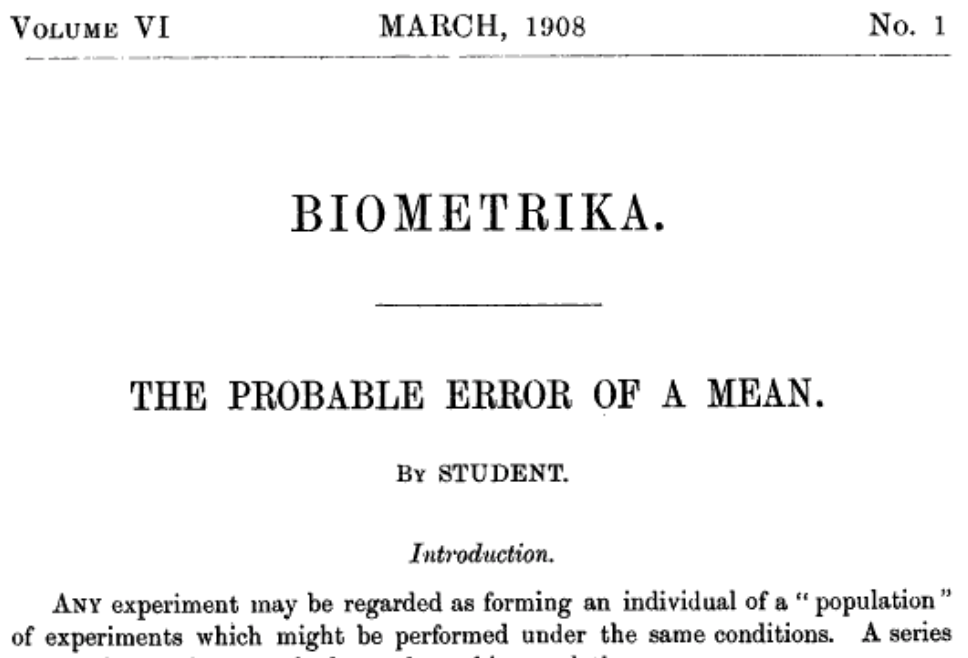
\includegraphics{student.png}
\end{marginfigure}
\begin{equation*}
	f_n(x) = \frac{1}{\sqrt{n \pi}} \frac{\Gamma((n+1) / 2)}{\Gamma(n/2)} \frac{1}{(1 + x^2 / n)^{(n + 1)/2}}
\end{equation*}
with respect to the Lebesgue density on $\R$.
If $T \sim \stu(n)$ we have $\E[T] = 0$ and $\var(T) = n / (n - 2)$ whenever $n > 2$.
Also, we have that $\stu(n) \gosto \nor(0, 1)$ as $n \rightarrow +\infty$ since $V / n \gopro 1$ (using the law of large numbers and Theorem~\ref{thm:slutsky}).

% \todo{Insert exercise on the Student distribution}

\paragraph{The Fisher distribution.}

Let $p, q \in \N \setminus \{ 0 \} $. If $U \sim \chisq(p)$ and $V \sim \chisq(q)$ are independent then
\begin{equation}
	\label{eq:fisher-definition}
	\frac{U / p}{V / q} \sim \fis(p, q)
\end{equation}
where $\fis(p, q)$ stands for the \emph{Fisher distribution} with density
\begin{equation*}
	f_{p, q}(x) = \frac{1}{x \beta(p/2, q/2)} \Big( \frac{px}{px + q} \Big)^{p/2} \Big(1 - \frac{px}{px + q} \Big)^{q/2} \ind{x \geq 0}
\end{equation*}
with respect to the Lebesgue measure on $\R$, where
\begin{equation}
	\label{eq:beta-function}
	\beta(a, b) = \frac{\Gamma(a) \Gamma(b)}{\Gamma(a + b)}  = \int_0^1 t^{a-1} (1 - t)^{b - 1} dt.
\end{equation}

\paragraph{The Beta distribution.} % (fold)

If $G_1 \sim \gam(a, \lambda)$ and $G_2 \sim \gam(b, \lambda)$ are independent then
\begin{equation*}
	\frac{G_1}{G_1 + G_2} \sim \bet(a, b)
\end{equation*}
where $\bet(a, b)$ is the Beta distribution with density
\begin{equation*}
	f_{a, b}(x) = \frac{1}{\beta(a, b)} x^{a - 1} (1 - x)^{b - 1} \ind{[0, 1]}(x)
\end{equation*}
with respect to the Lebesgue measure on $\R$, where the $\beta$ function is given by~\eqref{eq:beta-function}.
If $B \sim \bet(a, b)$ then $\E[B] = \frac{a}{a + b}$, $\var[B] = ab / ((a + b)^2 (a + b + 1))$ and $\mode(B) = (a - 1) / (a + b - 2)$ whenever $a, b > 1$.


\subsection{Joint distribution of $\wh \theta_n$ and $\wh \sigma^2$ and consequences}


In order to study the distribution of $\wh \theta_n$ and $\wh \sigma^2$, we need the following theorem, which proves that the projections onto orthogonal spaces of a Gaussian vector with isometric covariance are independent and Gaussian.
\begin{theorem}[Cochran theorem]
	\label{thm:cochran}
	Let $Z \sim \nor(0, \bI_n)$ and let $V_1, \ldots, V_k$ be orthogonal linear spaces of $\R^n$. Define the Gaussian vectors $Z_j = \bP_j Z := \proj_{V_j}(Z)$, where $\bP_j$ is the orthonormal projection matrix onto $V_j$. Then, we have that $Z_1, \ldots, Z_k$ are independent Gaussian vectors, and that
	\begin{equation}
		\norm{Z_j}^2 \sim \chisq(n_j)
	\end{equation}
	where $n_j = \dim(V_j)$ (note that $\sum_{j=1}^k n_j \leq n$).
\end{theorem}
The proof of Theorem~\ref{thm:cochran} is given in Section~\ref{sec:chap04_proofs} below.
Let us go back to the Gaussian linear model where $\by = \bX \theta + \beps$ with $\beps \sim \nor(0, \sigma^2 \bI_n)$.
We know that $\wh \theta_n$ is a Gaussian vector, as a linear transformation of the Gaussian vector $\by$, so that
\begin{equation*}
	\wh \theta_n \sim \nor(\theta, \sigma^2 (\bX^\top \bX)^{-1})
\end{equation*}
in view of Equations~\eqref{eq:mean-ols} and~\eqref{eq:var-ols}.
Moreover, we know from~\eqref{eq:residual-noise-relation} that $\by - \bX \wh \theta_n = (\bI_n - \bH) \beps = \proj_{V^\perp}(\beps)$ and that $\bX (\wh \theta_n - \theta) = \proj_V(\by - \bX \theta) = \proj_V(\beps)$.
Since $V \perp V^\perp$, Theorem~\ref{thm:cochran} entails that $\by - \bX \wh \theta_n$ and $\bX (\wh \theta_n - \theta)$ are independent, so that $\wh \sigma^2$ and $\wh \theta_n$ are also independent.
Moreover, since $\bX$ is full rank, we have $\dim V = d$ and $\dim V^\perp = n - d$, which entails with Theorem~\ref{thm:cochran} that
\begin{equation*}
	(n - d) \frac{\wh \sigma^2}{\sigma^2} = \norm{\proj_{V^\perp}(\beps / \sigma)}^2 \sim \chisq(n-d)
\end{equation*}
and
\begin{equation*}
	\frac{\norm{\bX(\wh \theta_n - \theta)}^2}{\sigma^2 } = \norm{\proj_{V}(\beps / \sigma)}^2 \sim \chisq(d).
\end{equation*}
This proves the following theorem.
\begin{theorem}
	\label{thm:gaussian-ols-distribution}
	Assume that $\bX$ is full rank and that $\by = \bX \theta + \beps$ with $\beps \sim \nor(0, \sigma^2 \bI_n)$. Put $\wh \by = \bX \wh \theta_n$ where $\wh \theta_n = (\bX^\top \bX)^{-1} \bX^\top \by$  and $\wh \sigma^2 = \norm{\by - \wh \by}^2 / (n-d)$. 
	Then, we have that $\wh \theta_n$ and $\wh \sigma^2$ are \emph{independent} and such that
	\begin{equation*}
		\wh \theta_n \sim \nor(\theta, \sigma^2 (\bX^\top \bX)^{-1}), \quad (n-d) \frac{\wh \sigma^2}{\sigma^2} \sim \chisq(n - d)
	\end{equation*}
	and $\norm{\bX(\wh \theta_n - \theta)}^2 / \sigma^2 \sim \chisq(d)$.
\end{theorem}

Theorem~\ref{thm:gaussian-ols-distribution} has many consequences for the inference of $\theta$ and $\sigma^2$ in the Gaussian linear model.
If $\sigma^2$ is known, the set
\begin{equation*}
	\cE = \Big \{ t \in \R^d : \frac{1}{\sigma^2} \norm{\bX (\wh \theta_n - t)}^2 \leq q_{\chisq(d)}(1 - \alpha)  \Big\}
\end{equation*}
where $q_{\chisq(d)}(1 - \alpha)$ is the quantile function of the $\chisq(d)$ distribution at $1 - \alpha$, is a \emph{confidence set}%
\sidenote{we call also $\cE$ a confidence \emph{ellipsoid}}
for $\theta$ in the Gaussian linear model at level $1 - \alpha$, since it satisfies by construction the coverage property $\P_\theta[ \theta \in \cE] = 1 - \alpha$.
If $\sigma^2$ is unknown (which is always the case), we use the fact%
\sidenote{We proved above that the numerator $\norm{\bX (\wh \theta_n - \theta)}^2 / \sigma^2$ has $\chisq(d)$ distribution while the denominator $(n-d) \wh \sigma^2 / \sigma^2$ has $\chisq(n - d)$ distribution and that both are independent, so that the definition~\eqref{eq:fisher-definition} of the Fisher distribution entails the result.}
that
\begin{equation*}
	\frac{\norm{\bX (\wh \theta_n - \theta)}^2}{d \wh \sigma^2} \sim \fis(d, n-d)
\end{equation*}
and consider instead the ellipsoid
\begin{equation}
	\label{eq:fisher-ellipsoid-construction}
	\Big \{ \theta \in \R^d : \frac{1}{d \wh \sigma^2} \norm{\bX (\wh \theta_n - \theta)}^2 \leq q_{\fis(d, n - d)}(1 - \alpha)  \Big\},
\end{equation}
which is by construction a confidence set at level $1 - \alpha$.
Note the cute trick involved in~\eqref{eq:fisher-ellipsoid-construction}: the ratio structure allows to cancel out $\sigma^2$, leading to a statistic that does not depend on $\sigma^2$, with a \emph{known} distribution.

% \todo{Y'a quand meme un probleme avec la notation $\theta$. Pourquoi pas $\sigma_0^2$ et en dessous y'en a plus. Faut decider quelque chose}

\paragraph{Confidence intervals.}

Both previous confidence regions provide coverage for the whole vector $\theta \in \R^d$.
We can also build confidence intervals for each coordinate of~$\theta$.
Indeed, we have $\theta_j = \theta^\top e_j$ where $e_j$ is the canonical basis vector with $1$ at coordinate $j$ and $0$ elsewhere. 
More generally, we can build a confidence interval for $a^\top \theta$ for any vector $a \in \R^d$.
We know that $a^\top(\wh \theta_n - \theta) \sim \nor(0, \sigma^2 a^\top (\bX^\top \bX)^{-1} a)$, so that
\begin{equation*}
	\frac{a^\top(\wh \theta_n - \theta)}{\sigma \sqrt{a^\top (\bX^\top \bX)^{-1} a}} \sim \nor(0, 1)
\end{equation*}
and let us recall that $\wh \theta_n$ and $\wh \sigma^2$ are independent and that $(n - d) \wh \sigma^2 / \sigma^2 \sim \chisq(n - d)$.
This entails
\begin{equation}
	\label{eq:ci-construction-gaussian-linear-model}
	\frac{a^\top(\wh \theta_n - \theta)}{\sqrt{\wh \sigma^2 a^\top (\bX^\top \bX)^{-1} a}} 
	\sim \stu(n - d)
\end{equation}
in view of the definition~\eqref{eq:student-definition} of the $\stu$ distribution.%
\sidenote{Note again the fact that the ratio structure in~\eqref{eq:ci-construction-gaussian-linear-model} cancels out $\sigma^2$ and that its \emph{exact} distribution is known, thanks to the assumption that the noise $\beps$ is Gaussian.}
This proves that the interval
\begin{equation*}
	I_{a, 1 - \alpha} = \Big[a^\top \wh \theta_n \pm q_{\stu(n-d)}(1 - \alpha/2) 
	\sqrt{\wh \sigma^2 a^\top (\bX^\top \bX)^{-1} a} \Big],
\end{equation*}
where $q_{\stu(n-d)}$ is the quantile function of the $\stu(n-d)$ distribution,
is a confidence interval for $a^\top \theta$ at level $1 - \alpha$, since it satisfies $\P_\theta[ a^\top \theta \in I_{a, 1 - \alpha}] = 1 - \alpha$ by construction.%
\sidenote{We use the fact that $q_{\stu(k)}(\alpha) = - q_{\stu(k)}(1 - \alpha)$ in this construction, since we know that $\stu(k)$ is a symmetrical distribution in view of~\eqref{eq:student-definition}.}
In particular, for $a = e_j$, we obtain that
\begin{equation}
	\label{eq:ci-gaussian-linear-coordinate}
	\Big[  (\wh \theta_n)_j \pm q_{\stu(n-d)}(1 - \alpha/2) \sqrt{\wh \sigma^2 ((\bX^\top \bX)^{-1})_{j, j}} \Big]
\end{equation}
is a confidence interval for $\theta_j$ at level $1 - \alpha$.

This confidence interval allows to build a test for the hypotheses $H_{0, j} : \theta_j = 0$ versus $H_{1, j} : \theta_j \neq 0$, which can help to quantify the statistical importance of the $j$-th feature in the considered dataset.
Also, a confidence interval for $\sigma^2$ can be easily built using the ancillary statistic $(n - d) \wh \sigma^2 / \sigma^2 \sim \chisq(n - d)$.

\begin{example}
	Consider $Y_1, \ldots, Y_n$ iid $\nor(\mu, \sigma^2)$. This is a Gaussian linear model since $\by = \mu \bone + \beps$ where $\beps \sim \nor(0, \sigma^2 \bI_n)$ and $\bone = [1 \cdots 1]^\top \in \R^n$.
	We have%
	\marginnote{using $(\bone^\top \bone)^{-1} \bone^\top \by = n^{-1} \sum_{i=1}^n Y_i$}
	$\wh \mu_n = \bar Y_n$ together with $\wh \sigma^2 = \frac{1}{n-1} \norm{\by - \bar Y_n \bone}^2 = \frac{1}{n-1} \sum_{i=1}^n (Y_i - \bar Y_n)^2$ and we know from Theorem~\ref{thm:gaussian-ols-distribution} that $\wh \mu_n$ and $\wh \sigma^2$ are independent and such that $\sqrt n (\wh \mu_n - \mu) / \sigma \sim \nor(0, 1)$ and $(n-1) \wh \sigma^2/\sigma^2 \sim \chisq(n-1)$ so that by definition of the $\stu(n-1)$ distribution we have
	\begin{equation*}
		\sqrt{\frac{n}{\wh \sigma^2}} (\wh \mu_n - \mu) \sim \stu(n-1)
	\end{equation*}
	so that we can build, using this ancillary statistic, a confidence interval and tests for $\mu$ when $\sigma^2$ is unknown.
\end{example}

\begin{example}
	Consider the \emph{simple} Gaussian linear regression model where $Y_i = a x_i + b + \eps_i$, with $a, b \in \R$, $x_1, \ldots, x_n \in \R$ and $\eps_i \sim \nor(0, \sigma^2)$ iid. This can be written as a linear model with
	\begin{equation*}
		\by = \bX \theta + \beps =
		\begin{bmatrix}
			1 & x_1 \\
			\vdots & \vdots \\
			1 & x_n
		\end{bmatrix}
		\begin{bmatrix}
			a \\
			b
		\end{bmatrix}
		+ \beps,
	\end{equation*}
	where we can compute explicitly $\wh \theta_n$ and $\wh \sigma^2$ and obtain their distributions using Theorem~\ref{thm:gaussian-ols-distribution}.
\end{example}

\paragraph{Prediction intervals.}

In the previous paragraph, we built confidence sets and intervals for the parameter $\theta \in \R^d$.
But, let us remind ourselves that one of the main usages of the linear model is to provide \emph{predictions} of the label $Y \in \R$ associated to a vector of features $X \in \R^d$.
Once the least-squares estimator $\wh \theta_n$ is computed, we predict the unknown label $Y_{\new}$ of a \emph{new}%
\sidenote{In the sense that $X_{\new}$ does not belong to the dataset $(X_1, Y_1), \ldots, (X_n, Y_n)$ with which $\wh \theta_n$ is trained}
 feature vector $X_{\new} \in \R^d$ using $\wh Y_{\new} = X_{\new}^\top \wh \theta_n$.
If we are willing to assume that the model is Gaussian, namely $\beps \sim \nor(0, \sigma^2 \bI_n)$, and that the unknown label $Y_{\new}$ satisfies the same Gaussian linear model $Y_{\new} = X_{\new}^\top \theta + \eps_{\new}$ where $\eps_{\new}$ is independent of $\beps$ and
 $\eps_{\new} \sim \nor(0, \sigma^2)$, then we know that $\wh Y_{\new}$ and $Y_{\new}$ are independent Gaussian random variables, so that $\wh Y_{\new} - Y_{\new}$ is also Gaussian, and
 $\E_\theta[\wh Y_{\new} - Y_{\new}] = X_{\new}^\top \E_\theta[\wh \theta_n] - X_{\new}^\top \theta = 0$ and
 \begin{align*}
 	\var[\wh Y_{\new} - Y_{\new}] &= \var[\wh Y_{\new}] + \var[Y_{\new}] \\
 	&= \sigma^2 (X_{\new}^\top (\bX^\top \bX)^{-1} X_{\new} + 1),
 \end{align*}
which means that
\begin{equation*}
	\wh Y_{\new} - Y_{\new} \sim \nor\big(0, \sigma^2 (1 + X_{\new}^\top (\bX^\top \bX)^{-1} X_{\new})\big)
\end{equation*}
and using again the fact that $\wh \sigma^2$ and $\wh \theta_n$ are independent and $(n-d) \wh \sigma^2 / \sigma^2 \sim \chisq(n -d)$ we obtain
\begin{equation*}
	\frac{\wh Y_{\new} - Y_{\new}}{\sqrt{\wh \sigma^2  (1 + X_{\new}^\top (\bX^\top \bX)^{-1} X_{\new}) }} \sim \stu(n-d)
\end{equation*}
so that the interval
\begin{align*}
	I_{\new}(X_{\new}) = \Big[ \wh Y_{\new} \pm &q_{\stu(n-d)}(1 - \alpha / 2) \\
	& \times \sqrt{\wh \sigma^2  (1 + X_{\new}^\top (\bX^\top \bX)^{-1} X_{\new}) } \Big]
\end{align*}
is a prediction interval at level $1 - \alpha$, since we have by construction $\P[Y_{\new} \in I_{\new}(X_{\new})] = 1 - \alpha$.


\subsection{The Fisher test} % (fold)
\label{sub:the_fisher_test}

Using the confidence interval~\eqref{eq:ci-construction-gaussian-linear-model} we can test $H_0 = \theta_1 = \theta_2$ by using $a = [1, -1, 0, \ldots, 0]$. 
But, how can we test $H_0 : \theta_1 = \theta_2 = 0$ or more generally a \emph{multiple} null hypothesis such as
\begin{equation}
	\label{eq:fisher-test-multiple-null-example}
	H_0 : \theta_1 = \cdots = \theta_k = 0
\end{equation}
for $k = 2, \ldots, d$ ?
If we fix $j \in \{ 1, \ldots, k\}$ and consider the simple null hypothesis $H_{0, j} : \theta_j = 0$ versus the alternative $H_{1, j} : \theta_j \neq 0$, we know thanks to the confidence interval~\eqref{eq:ci-gaussian-linear-coordinate} together with Proposition~\ref{prop:ci-and-tests} that the test with rejection set 
\begin{equation*}
	R_{j, \alpha} = \Big\{ |(\wh \theta_n)_j| > q_{\stu(n-d)}(1 - \alpha/2) \sqrt{\wh \sigma^2 ((\bX^\top \bX)^{-1})_{j, j}} \Big\}
\end{equation*}
has level $\alpha$, namely $\P_{\theta_j = 0}[R_{j, \alpha}] = \alpha$, for any $j=1, \ldots, k$.
So, an approach to test the multiple hypothesis $H_0$ given by~\eqref{eq:fisher-test-multiple-null-example} would be to consider a rejection set given by the \emph{union} of the individual $R_{j, \alpha}$, with a decreased level $\alpha / k$, since
\marginnote[*2]{The notation $\P_{H_0}$ means that we compute the probability assuming that $H_0$ holds, namely $\theta_1 = \cdots = \theta_k = 0$}
\begin{equation*}
	\P_{H_0} \Big [ \bigcup_{j=1}^k R_{j, \alpha / k} \Big] 
	\leq \sum_{j=1}^k \P_{\theta_j = 0} [ R_{j, \alpha / k} ] \leq k \times \alpha / k = \alpha,
\end{equation*}
so that the test with rejection set $\cup_{j=1}^k R_{j, \alpha / k}$ for the null hypothesis~\eqref{eq:fisher-test-multiple-null-example} has indeed level $\alpha$.
This strategy, which relies on a union bound for the construction of a \emph{multiple test} is called the Bonferroni correction.%
\sidenote{This is called Bonferroni correction, although this strategy is due to Olive Jean Dunn (1915–2008) who worked on statistical testing for biostatistics.}
It is the simplest approach for multiple testing, more about multiple tests will follow later in this book.

This Bonferroni correction requires to replace the individual levels $\alpha$ of each test by the decreased $\alpha /k$, where $k$ is the number of null hypotheses to be tested.
If $k$ is large, this is a large decrease, and we expect a large deterioration of the power of each individual test.
In the Gaussian linear model, we can do much better than this, thanks to the Fisher test.

Let us continue with the null assumption~\eqref{eq:fisher-test-multiple-null-example} and put $\Theta_0 = \{ \theta \in \R^d : \theta_1 = \cdots = \theta_k = 0 \}$. 
Let us that recall that $V = \spa(\bX) = \{ \bX u : u \in \R^d\}$ and introduce $W = \{ \bX u : u \in \Theta_0 \}$. 
Note that $\theta \in \Theta_0$ means that $\bA \theta = 0$ with $\bA = [\bI_k \bO_{k, d-k}]$ corresponding to the horizontal concatenation of the identity matrix on $\R^k$ and a $k \times (d-k)$ zero matrix.
More generally, we can consider a multiple testing problem with null hypothesis
\begin{equation}
	\label{eq:fisher-null-hypothesis}
	H_0 : \theta \in \Theta_0 \quad \text{with} \quad \Theta_0 = \ker(\bA),
\end{equation}
where $\bA$ is a $k \times d$ matrix of rank $k$.
The idea of the Fisher test is to use the fact that $\theta \in \Theta_0$ means that $\bX \theta$ lives in a linear subset $W \subset V$, of dimension $d - k < d$, and to detect statistically this fact.

The Fisher test uses a geometric solution to this testing problem: we decompose $\R^n$ as the following direct sums
\begin{equation*}
	\R^n = V^\perp \oplus V = V^\perp \oplus W \oplus W',
\end{equation*}
where we note that $\dim(V^\perp) = n - d$, $\dim(W) = d - k$ and $\dim(W') = k$, where $W = \{ \bX \theta : \theta \in \Theta_0 \} \subset V$.
Consider now the projections $\proj_V(\by)$ and $\proj_W(\by)$ of $\by$ onto $V$ and its subspace~$W$.
Pythagora's theorem entails that%
\begin{marginfigure}%
\begin{tikzpicture}[scale=1]%
\draw [dashed, thick, color=gray!80] (2, 2) -- ++(-2, -1.2) -- ++(4.5, -1);%
\fill [color=gray!10] (0, 0.8) -- ++(4.8, 2.88) -- ++(0, -3.95);%
\draw (4.5, 3) node {$V$};%
\draw (3, 3) node[right] {$\by$};%
\draw (3, 3) node {$\bullet$};%
\draw (3, 3) -- (3, 1);%
\draw (3, 1) node[left]{$\proj_V(\by)\;$};%
\draw (3.4, 0.8) node[below] {$W$};
\draw[dashed, thick] (2.6, 0.5) -- ++(2, 1);
\draw (4.2, 1.3) node {$\bullet$};
\draw (4.2, 1.3) node[right] {$\; \proj_W(\by)$};
\draw (4.34, 1.37) -- ++(-0.12, 0.17) -- ++(-0.14, -0.07);
\draw (3, 3) -- (4.2, 1.3);
\draw (3, 1) node {$\bullet$};%
\draw (3, 1.2) -- ++(-0.18, 0.04) -- ++(0, -0.2);%
\end{tikzpicture}%
\caption{Geometric construction of the Fisher test}
\end{marginfigure}%
\begin{equation*}
	\norm{\by - \proj_W(\by)}^2 = \norm{\by - \proj_V(\by)}^2 + \norm{\proj_V(\by) - \proj_W(\by)}^2
\end{equation*}
since $\by - \proj_V(\by) \perp \proj_V(\by) - \proj_W(\by) \in V$, so that 
\begin{equation*}
	\norm{\proj_V(\by) - \proj_W(\by)}^2 = \norm{\by - \proj_W(\by)}^2 - \norm{\by - \proj_V(\by)}^2.
\end{equation*}
Recall that $\proj_V(\by) = \bX \wh \theta_n$ where $\wh \theta_n$ is the least squares estimator while $\proj_W(\by) = \bX \wt \theta_n$ where $\wt \theta_n$ is the least squares estimator computed under $H_0$, namely $\wt \theta_n = \argmin_{\theta \in \Theta_0} \norm{\by - \bX \theta}^2$.
This is where the trick of the test comes into the picture: the quantity $\proj_V(\by) - \proj_W(\by)$ behaves very differently whenever $H_0$ holds or not. 
Indeed, \emph{under $H_0$}, namely when $\bX \theta \in W$, we have
\begin{align*}
	\proj_V(\by) - \proj_W(\by) = \proj_{W'} (\by) &= \proj_{W'}(\bX \theta) + \proj_{W'}(\beps) \\
	&= \proj_{W'}(\beps),
\end{align*}
since in this case $\bX \theta \in W \perp W'$, while $\proj_{W'}(\bX \theta) \neq 0$ when $\theta \notin \Theta_0$.
So, under $H_0$, we have that $(\proj_V(\by) - \proj_W(\by)) / \sigma = \proj_{W'}(\beps / \sigma)$ while 
$(\by - \proj_V(\by)) / \sigma = \proj_{V^\perp}(\beps / \sigma)$. 
Therefore, since $V^\perp \perp W'$, Theorem~\ref{thm:cochran} together with the definition~\eqref{eq:fisher-definition} of the Fisher distribution proves that
\begin{align*}
	\frac{\norm{\proj_V(\by) - \proj_W(\by)}^2 / k}{\norm{\by - \proj_V(\by)}^2 / (n - d)} 
	&= \frac{\norm{\proj_{W'}(\beps / \sigma)}^2 / k}{\norm{\proj_{V^\perp}(\beps / \sigma)}^2 / (n-d)} \\
	&\sim \fis(k, n-d)
\end{align*}
under the $H_0$ hypothesis.%
\sidenote{Theorem~\ref{thm:cochran} tells us that under $H_0$, we have that $\norm{\proj_{W'}(\beps / \sigma)}^2 \sim \chisq(k)$, that $\norm{\proj_{V^\perp}(\beps / \sigma)}^2 \sim \chisq(n - d)$ and that both are independent.}
This can be rewritten, under $H_0$, as 
\begin{align*}
	\frac{\big(\norm{\by - \bX \wt \theta_n}^2 - \norm{\by - \bX \wh \theta_n}^2\big) / k}
	{\norm{\by - \bX \wh \theta_n}^2 / (n - d)} 
	&= \frac{\norm{\bX (\wh \theta_n - \wt \theta_n)}^2}{k \wh \sigma^2} \\
	&\sim \fis(k, n-d).
\end{align*}
Once again, the ratio structure of the ancillary statistic cancels out the unknown $\sigma^2$.
We can conclude now that the Fisher test with rejection region
\begin{equation*}
	R_\alpha = \bigg\{  \frac{\norm{\bX (\wh \theta_n - \wt \theta_n)}^2}{k \wh \sigma^2}  \geq q_{\fis(k, n-d)}(1 - \alpha)  \bigg\}
\end{equation*}
has level $\alpha$ for the null hypothesis~\eqref{eq:fisher-null-hypothesis}, namely that $\sup_{\theta \in \Theta_0} \P_\theta[R_\alpha] = \alpha$.
This test is pretty intuitive and can be understood as follows: if $\theta \in \Theta_0$ then both estimators $\wh \theta_n$ and $\wt \theta_n$ should be close, and $\bX (\wh \theta_n - \wt \theta_n)$ should be, consequently, ``small'', the small miracle being that, in the Gaussian linear model, we can perfectly quantify how small.

\begin{example}
	Consider a Gaussian linear model $Y_i = X_i^\top w + b + \eps_i$ where $w \in \R^{d-1}$, where $b \in \R$ is an intercept%
	\marginnote{In practice, you should always include an intercept in a linear model, unless you have a good reason in not doing so.}
	and the noise $\eps_i \sim \nor(0, \sigma^2)$ is iid. Using the same notations as before, we can rewrite this as $\by = \bX \theta + \beps$ where $\beps \sim \nor(0, \sigma^2 \bI_n)$, where $\theta = [b, w^\top]^\top \in \R^d$ and where $\bX = [\bone X^1 \cdots X^{d-1}]$ is assumed to be full-rank. In this model, we wish to test if the features $X_i$ are useful or if a constant intercept is enough to predict $Y$.
	Namely, we want to test $H_0 : w = 0$ versus $H_1 : w \neq 0$, namely $H_0 : \theta_2 = \cdots = \theta_d = 0$. This can be done using the Fisher test, putting $W = \spa(\bone)$ so that $\dim(W) = 1 = d - k$ with $k = d - 1$ and $\Theta_0 = \{ \theta \in \R^d : \theta_2 = \cdots = \theta_d = 0 \}$. 
	Since $\proj_W(\by) = \bar Y_n \bone_n$, the least-squares estimator under $H_0$ is $\wt \theta_n = \bar Y_n \bone_d$, so that the rejection set at level $\alpha$ of the Fisher test writes in this case 
	\begin{equation}
		\label{eq:linreg-f-test}
		\bigg\{  \frac{\norm{\bX \wh \theta_n - \bar Y_n \bone_n}^2}{(d - 1) \wh \sigma^2}  
		\geq q_{\fis(d-1, n-d)}(1 - \alpha)  \bigg\},
	\end{equation}
	with the same notations as before. The $p$-value of this test can be therefore used as a quantification of how much the features are informative globally to predict the label using a linear model, versus a constant intercept. This test is known as the \emph{$F$-test} for linear regression and the statistic used in~\eqref{eq:linreg-f-test} is known as the \emph{$F$-statistic}.
\end{example}

\subsection{Analysis of variance} % (fold)
\label{sub:analysis_of_variance}

Consider independent random variables $X_{i, j} \sim \nor(m_i, \sigma^2)$ for $i=1, \ldots, k$ and $j=1, \ldots, n_i$, namely, we observe $k$ Gaussian iid samples with respective sizes $n_1, n_2,\dots, n_k$, denoted
\begin{equation*}
	X_{i, \bullet} = [X_{i, 1} \cdots X_{i, n_i}]^\top \in \R^{n_i}.
\end{equation*}
The parameters $m = [m_1 \cdots m_k]^\top \in \R^k$ and $\sigma^2 > 0$ are unknown, and we want to build a test for the hypotheses
\begin{equation*}
  H_0 : m_1 = m_2 = \cdots = m_k  \quad \text{against} \quad H_1 : \exists i \neq i': m_i \neq m_{i'},
\end{equation*}
namely, we want to test if all the samples share the same expectation.
We consider the random vector
\begin{equation*}
	X = [X_{1, \bullet}^\top \cdots X_{k, \bullet}^\top]^\top \in \R^n
\end{equation*}
where $n = \sum_{i=1}^k n_i$, which is the vertical concatenation of the random vectors $X_{1, \bullet}, \ldots, X_{k, \bullet}$.
First, we observe that 
\begin{equation*}
 \mu = \E [X] = 
 \begin{bmatrix}
  m_1 \cdots m_1 \, m_2 \cdots m_2 \cdots m_k \cdots m_k
 \end{bmatrix}^\top \in \R^n
\end{equation*}
belongs to a linear space $E$ of dimension $k$, since $\mu = \sum_{i=1}^k m_i e_i$ where $e_1 \in \R^n$ is the vector with $n_1$ first entries equal to $1$ and the others equal to $0$, $e_2$ the vector with the first $n_1$ entries equal to 0, the next $n_2$ entries equal to $1$ and all others equal to $0$, up to $e_k$ with $n_k$ last entries equal to $1$ and all others $0$, so that $E = \spa(e_1, \ldots, e_k)$ where the $e_i$ are orthogonal.
The orthogonal projection of $X$ onto $E$ is therefore given by
\begin{equation*}
	X_E := \proj_E(X) = \sum_{i=1}^k \frac{1}{n_i} \inr{X, e_i} e_i = \sum_{i=1}^k \bar X_{i, \bullet} e_i
\end{equation*}
where $\bar X_{i, \bullet} := \frac{1}{n_i} \inr{X, e_i} = \frac{1}{n_i} \sum_{j=1}^{n_i} X_{i, j}=$ the average of the $i$-th sample.
The null hypothesis writes $H_0:  \mu \in F$, where $F = \spa(\bone)$ is a linear subspace of $E$ with dimension $1$.
\marginnote{The vector $\bone \in \R^n$ has all its entries equal to $1$.}
The orthogonal projection of $X$ onto $F$ is given by
\begin{equation*}
	X_F := \proj_F(X) = \bar X \bone
\end{equation*}
where $\bar X = \frac 1n \sum_{i=1}^k \sum_{j=1}^{n_i} X_{i, j}$ is the average over all the samples.

We can use the Fisher test to test for $H_0$.
We write $X = \mu + \beps$ where $\beps \sim \nor(0, \sigma^2 \bI_n)$ and decompose 
\begin{equation*}
	\R^n = E^\perp \oplus E = E^\perp \oplus F \oplus W.
\end{equation*}
Let us recall that the idea of the Fisher test is to exploit the fact that $X_E - X_F = X_W = \proj_W(\mu + \beps) = \proj_W(\mu) + \proj_W(\beps)$ and that \emph{whenever $H_0$ is true}, namely $\mu \in F$, we have $\proj_W(\mu) = 0$, so that $\frac{1}{\sigma^2} \| X_E - X_F \|^2 = \| \proj_W( \beps / \sigma) \|^2$. 
Moreover, $X - X_E = \proj_{E^\perp}(X) = \proj_{E^\perp}(\mu + \beps) = \proj_{E^\perp}(\beps)$ since $\mu \in E$ so $\frac{1}{\sigma^2} \| X - X_E \|^2 = \| \proj_{E^\perp}( \beps / \sigma) \|^2$.
Since $\beps / \sigma \sim \nor(0, \bI_n)$ we know from Theorem~\ref{thm:cochran} that
\begin{equation*}
	\| \proj_W( \beps / \sigma) \|^2 \sim \chi^2(k-1) \quad \text{and} \quad
\| \proj_{E^\perp}( \beps / \sigma) \|^2 \sim \chi^2(n-k)
\end{equation*}
since $\dim(E^\perp) = n - k$ and $\dim(W) = k-1$ and that these are independent variables since $E^\perp \perp W$.
This proves that
\begin{equation*}
  T = \frac{\| X_E - X_F \|^2 / (k-1)}{\| X - X_E \|^2 / (n-k)} \sim \fis(k-1, n-k),
\end{equation*}
so we can consider the Fisher test with rejection region 
\begin{equation*}
	R = \{ T \geq q_{\fis(k-1, n-k)}(1 - \alpha) \}.
\end{equation*}
We can rewrite the statistic $T$ in a much more interpretable way.
First, we can write
\begin{align*}
  \| X - X_E \|^2 &= \sum_{i=1}^k \sum_{j=1}^{n_i} (X_{i, j} - \bar X_{i, \bullet})^2 \\
  &= \sum_{i=1}^k n_i  \frac{1}{n_i} \sum_{j=1}^{n_i} (X_{i, j} - \bar X_{i, \bullet})^2 =: n V_{\text{intra}},
\end{align*}
where $V_{\text{intra}}$ is the so-called \emph{intra-class variance}%
\sidenote{A \emph{class} corresponds here to a sample $i$}
which corresponds to the average of the weighted%
\sidenote{weighted by the sample proportions $n_i / n$ for $i=1, \ldots, k$}
 variances $\frac{1}{n_i} \sum_{j=1}^{n_i} (X_{i, j} - \bar X_{i, \bullet})^2$ of each sample  $i=1, \ldots, k$ and second, we have
\begin{equation*}
  \| X_E - X_F \|^2 = \sum_{i=1}^k n_i (\bar X_{i, \bullet} - \bar X)^2 =: n V_{\text{inter}},
\end{equation*}
where $V_{\text{inter}}$ is the \emph{inter-class variance} which corresponds to the weighted variance of the averages of each sample.
This explains the name ANOVA (ANalysis Of VAriance), since the Fisher test uses here the test statistic
\begin{equation*}
  T = \frac{V_\text{inter} / (k-1)}{V_\text{intra} / (n - k)},
\end{equation*}
which is the ratio between the inter and intra-class variances $V_{\text{inter}}$ and $V_\text{intra}$.


\section{Leverages} % (fold)
\label{sec:leverages}

Let us go back now to the general linear model.
We know that the residual vector $\wh \beps = \by - \wh \by = (\bI - \bH) \by$ is such that $\E[\wh \beps] = 0$ and $\var[\beps] = \sigma^2 (\bI - \bH)$, so that
\begin{equation*}
	\wh \beps_i \sim \nor(0, \sigma^2 (1 - h_{i,i})) \text{ where } h_{i, i} = \bH_{i, i} = X_i^\top (\bX^\top \bX)^{-1} X_i.
\end{equation*}
We know that $h_{i, i} \in [0, 1]$ since $\bH$ is an orthonormal projection matrix.%
\sidenote{Using $\bH^2 = \bH$ and $\bH^\top \bH$ we get $h_{i, i} = (\bH^2)_{i, i} = h_{i, i}^2 + \sum_{i' \neq i} h_{i, i'}^2$ so that $h_{i, i} (1 - h_{i, i}) \geq 0$.}
We call $h_{i, i}$ the \emph{leverage score} of sample $i$. We say that $i$ has small leverage whenever $h_{i, i}$ is close to zero while we say that is as a large leverage when $h_{i, i}$ is close to $1$, since in this case the contribution of sample $i$ to the linear model is important, since $\wh \beps_i \approx 0$.
Also, we note that 
\begin{equation*}
	h_{i, i} = \frac{\partial \wh Y_i}{\partial Y_i}
\end{equation*}
since $\wh \by = \bH \by$, namely $\wh Y_i = \sum_{j=1}^d \bH_{i, j} Y_j$.
So, the leverage $h_{i, i}$ can be understood as a quantity that measures the ``self-sensitivity'' to its prediction, namely the influence of $Y_i$ on the computation of $\wh Y_i$.
We will see also in the next Section that the leverage score is a very important concept as it is deeply connected to the \emph{theoretical performance} of the least-squares estimation procedure.
% \todo{Insert studentized residuals ?}

\section{Least squares are minimax optimal} % (fold)
\label{sec:optimality_of_the_least_squares}


While the previous contents is quite classical and well-known, the results provided in this Section are surprisingly recent and coming from the PhD manuscript of J. Mourtada, see~\sidecite{mourtadaphd, mourtada_leastsquares}.

Let us come back to the general case where $(X_1, Y_1), \ldots, (X_n, Y_n)$ are iid with same distribution as $(X, Y)$, with $X \in \R^d$ and $Y \in \R$ such that $\E \norm{X}^2 < +\infty$ and $\E[Y^2] < +\infty$. 
Also, we assume that $\P_X$ is non-degenerate, as explained in Theorem~\ref{thm:least-squares-existence} and we assume that
\begin{equation*}
	\bSigma := \E[X X^\top] \succ 0,
\end{equation*}
namely that $\bSigma$ is invertible.
We consider again the linear model (not Gaussian, the results stated here are much more general than that).
Given $\sigma^2$ and $\P_X$, we consider the following classes of distribution $\P_{X, Y}$ on $(X, Y)$.

\begin{definition}
	We consider the set $\cC(\P_X, \sigma^2)$ of joint distributions $\P_{X, Y}$ such that $X \sim \P_X$ and
	\begin{equation*}
		Y = X^\top \theta^\star + \eps
	\end{equation*}
	for some $ \theta^\star \in \R^d$, where $\eps$ satisfies $\E[\eps | X] = 0$ and $\E[\eps^2 | X] \leq \sigma^2$ almost surely. We consider also the set $\cG(\P_X, \sigma^2) \subset \cC(\P_X, \sigma^2)$ where we assume additionally that $\eps | X \sim \nor(0, \sigma^2)$.
\end{definition}
The set $\cC(\P_X, \sigma^2)$ is a general set of joint distributions on $(X, Y)$ with fixed marginal distribution $\P_X$ and such that $Y$ is a linear function of $X$ plus a noise $\eps$ which is conditionally centered and with finite variance. 
The set $\cG(\P_X, \sigma^2)$ is the same as $\cC(\P_X, \sigma^2)$, but where we assume that $\eps$ is centered Gaussian and independent of $X$.

We consider the quadratic risk
\begin{equation*}
	R(\theta) := \E [ (Y - X^\top \theta)^2] = \int (y - x^\top \theta)^2 \P_{X, Y}(dx, dy).
\end{equation*}
It is easy to see that
\begin{equation*}
	\theta^\star = \argmin_{\theta \in \R^d} R(\theta) = \bSigma^{-1} \E[Y X].
\end{equation*}
Our aim here is to find an estimator%
\sidenote{Namely, a measurable function of $(X_1, Y_1), \ldots, (X_n, Y_n)$.}
$\wh \theta$ of $\theta$  such that the \emph{excess risk}
\begin{equation*}
	\cE(\wh \theta) := R(\wh \theta) - R(\theta^\star)
\end{equation*}
is \emph{minimal}.
Note that if $(X, Y) \sim P$ with $P \in \cC(\P_X, \sigma^2)$, then
\begin{align*}
	\cE(\theta) &= \E [ (Y - X^\top \theta)^2 - (Y - X^\top \theta^\star)^2] \\
	&= \E [ (\theta^\star - \theta)^\top X (2 Y - X^\top (\theta + \theta^\star))] \\
	&= \E [ (\theta^\star - \theta)^\top X (X^\top (\theta^\star - \theta) + 2 \eps)] \\
	&= \E [ (\theta^\star - \theta)^\top X X^\top (\theta^\star - \theta)] \\
	&= \norm{\theta^\star - \theta}_{\bSigma}^2,
\end{align*}%
\marginnote[*-5]{We use here the fact that $Y = X^\top \theta^\star + \eps$ and that $\E[\eps | X] = 0$ almost surely.}%
where we introduced $\norm{x}_{\bSigma}^2 = x^\top \bSigma x$, which is a norm since we assumed $\bSigma \succ 0$.
Whenever $(X, Y) \sim P$ with $P \in \cC(\P_X, \sigma^2)$ we will therefore write
\begin{equation*}
	\cE(\theta) = R(\theta) - R(\theta^\star) = \norm{\theta - \theta^\star}_{\bSigma}^2
\end{equation*}
and whenever $\wh \theta$ depends on the data $(X_1, Y_1), \ldots, (X_n, Y_n)$, we can consider, since $(X, Y)$ is an independent copy with the same distribution,
\begin{equation*}
	\E [ \cE(\wh \theta) ]
\end{equation*}
where this expectation is with respect to $P^{\otimes n}$, for the randomness coming from the data. 
We can consider now the \emph{minimax risk} for a set $\cP$ of distributions:
\begin{equation*}
	\inf_{\wh \theta} \sup_{P \in \cP} \E[\cE(\wh \theta)].
\end{equation*}
The infimum is taken over any possible estimator, namely any statistic of the data, while the sup is over all distributions in $\cP$. Hence the name minimax, since we look at the worst-case excess risk over the considered set $\cP$, but we consider the best possible estimator (with the inf).
Since $\cG(\P_X, \sigma^2) \subset \cC(\P_X, \sigma^2)$, the minimax risk of the former is smaller than the one of the latter.

Some remarks and extra notations are required before we can state the main result of the section.
\begin{itemize}
	\item The linear model is \emph{well-specified} here, since we assume that $Y = X^\top \theta^\star + \eps$ almost surely with $\E[\eps | X] = 0$, so that there is no approximation term of $\E[Y | X]$ by $X^\top \theta^\star$.
	\item For the class $\cP = \cC(\P_X, \sigma^2)$, we expect a \emph{minimax estimator}%
	\marginnote{A minimax estimator is an estimator achieving the minimax risk.}
	 $\wh \theta$ to depend both on $\P_X$ and $\sigma^2$. Quite surprisingly, we will see that it is not the case.
\end{itemize}
Let us introduce
\begin{equation*}
	\wh \bSigma = \frac 1n \sum_{i=1}^n X_i X_i^\top = \frac 1n \bX^\top \bX
\end{equation*}
 and let us introduce also the ``whitened'' random vectors $\wt X_i = \bSigma^{-1/2} X_i$ (so that $\E[\wt X_i (\wt X_i)^\top] = \bI_d$) and define
\begin{equation*}
	\wt \bSigma = \frac 1n \sum_{i=1}^n \wt X_i \wt X_i^\top = \bSigma^{-1/2} \wh \bSigma \bSigma^{-1/2}.
\end{equation*}
The following theorem holds.
\begin{theorem}
	\label{thm:least-squares-minimax}
	Assume that $\P_X$ is non-degenerate, that $n \geq d$ and that $\sigma^2 > 0$. 
	Then
	\begin{equation}
		\label{eq:least-squares-minimax}
		\begin{split}
			\inf_{\wh \theta} \sup_{P \in \cC(\P_X, \sigma^2)} \E [\cE(\wh \theta)] 
			&= \inf_{\wh \theta} \sup_{P \in \cG(\P_X, \sigma^2)} \E [\cE(\wh \theta)] \\
			&= \frac{\sigma^2}{n} \E [\tr(\wt \bSigma ^{-1})].
		\end{split}
	\end{equation}
	Furthermore, the infimum in the minimax risk is achieved by the ordinary least squares estimator~\eqref{eq:least-squares-estimator}.
\end{theorem}

The proof of Theorem~\ref{thm:least-squares-minimax} is done in two steps.
The first step, which proves that the ordinary least squares estimator satisfies the upper bound in~\eqref{eq:least-squares-minimax}, is given in Section~\ref{sec:chap04_proofs} below.
Since the proof of the lower bound requires extra tools from Bayesian statistics, it will be provided in Section~\ref{sec:sec:chap05_proofs} of Chapter~\ref{chap:bayesian_statistics}.

This theorem deserves several remarks.
\begin{itemize}
	\item The theorem proves that the least-squares estimator is, in a fairly general setting, \emph{minimax optimal}: it cannot be improved by another estimator, uniformly over the set of distributions $\cC(\P_X, \sigma^2)$.
	\item The Gaussian noise, namely the class $\cG(\P_X, \sigma^2)$ ``saturates'' the minimax risk, and corresponds to the \emph{least favorable} distribution in the minimax sense.
	\item The minimax risk is invariant by a linear transformation of the features vectors: it is unchanged if one replaces $X_i$ by $X_i' = \bA X_i$ for some deterministic invertible matrix $\bA$. Indeed we have in this case $\wh \bSigma' = \frac 1n \sum_{i=1}^n X_i' X_i'^\top = \bA \wh \bSigma \bA^\top$ so that $(\wh \bSigma')^{-1} \bSigma' = (\bA^\top)^{-1} (\wh \bSigma)^{-1} \bSigma \bA^\top$ which proves that $(\wh \bSigma')^{-1} \bSigma'$ and $(\wh \bSigma)^{-1} \bSigma$ are congruent matrices, so that they share the same trace, namely $\tr((\wh \bSigma')^{-1} \bSigma') = \tr((\wh \bSigma)^{-1} \bSigma)$, and the minimax risk is indeed invariant when replacing $X_i$ by $\bA X_i$. This is of course expected, since the supremum is over linear functions.
\end{itemize}
A lower bound for $\sigma^2 \E [\tr(\wt \bSigma ^{-1})] / n$ can be easily obtained thanks to the following proposition.
\begin{proposition}
	\label{prop:trace-inv-convex}
	The function $\bA \mapsto \tr( \bA^{-1})$ is convex on the cone of positive definite matrices.
\end{proposition}
The proof of Proposition~\ref{prop:trace-inv-convex} is given in Section~\ref{sec:chap04_proofs} below.
By combining Proposition~\ref{prop:trace-inv-convex} and Jensen's inequality, we obtain
\begin{equation*}
	\E [\tr({\wt \bSigma}^{-1}) ] \geq \tr (\E [\wt \bSigma]^{-1} ),
\end{equation*}
but $\E[\wt \bSigma] = \bSigma^{-1/2} \E [\wh \bSigma] \bSigma^{-1/2} = \bI_d$, so the lower bound 
\begin{equation*}
	\E [\tr( \wt \bSigma^{-1})] \geq d
\end{equation*}
holds, and consequently the minimax risk satisfies
\begin{equation}
	\label{eq:first-explicit-minimax-lower-bound}
	\inf_{\wh \theta} \sup_{P \in \cC(\P_X, \sigma^2)} \E [\cE(\wh \theta)] 
	= \frac{\sigma^2}{n} \E [\tr(\wt \bSigma ^{-1})] \geq \sigma^2 \frac dn.
\end{equation}

We can also provide another expression for $\E [\tr (\wt \bSigma^{-1})]$ using the leverage scores we discussed in Section~\ref{sec:leverages}.
Let us recall at this point that since $\P_X$ is non-degenerate, and if $X_1, \ldots X_{n+1}$ are iid and distributed as $\P_X$, we have $\sum_{i=1}^{n+1} X_i X_i^\top \succ 0$.
\begin{theorem}
	\label{thm:minimax-leverage}
	Under the same assumptions as that of Theorem~\ref{thm:least-squares-minimax}, the minimax risk can be written as
	\begin{equation*}
		\frac 1n \E [\tr ( \wt \bSigma^{-1}) ] = \E \Big[ \frac{\wh \ell_{n+1}}{1 - \wh \ell_{n+1}} \Big]
	\end{equation*}
	where $\wh \ell_{n+1}$ is the leverage of one data point among $n+1$ given by
	\begin{equation*}
		\wh \ell_{n+1} = X_{n+1}^\top \Big( \sum_{i=1}^{n+1} X_i X_i^\top \Big)^{-1} X_{n+1},
	\end{equation*}
	where $X_1, \ldots, X_n, X_{n+1}$ are iid with distribution $\P_X$.
\end{theorem}

The proof of Theorem~\ref{thm:minimax-leverage} is given in Section~\ref{sec:chap04_proofs} below.
Let us recall that $\wh \ell_{n+1} = \partial \wh Y_{n+1} / \partial Y_{n+1}$ where $\wh Y_{n+1} = X_{n+1}^\top \wh \theta_{n+1}$ where $\wh \theta_{n+1}$ is the ordinary least squares estimator computed on the $n+1$ samples $(X_1, Y_1), \ldots, (X_{n+1}, Y_{n+1})$. 
This theorem entails that the minimax risk, which measures the complexity of the estimation problem,  is completely determined by the leverage score. 
Even more than that, it is the expected value of a convex function of $\wh \ell_{n+1}$, so that the minimax risk is small when $\wh \ell_{n+1}$ is small, and gets larger with a large $\wh \ell_{n+1}$, which is natural since in such a case, the regression problem is more difficult. 

A corollary of Theorem~\ref{thm:minimax-leverage} is an improved lower bound compared to the previous $\sigma^2 d / n$.

\begin{corollary}
	\label{cor:proof-lower-bound-leverage}
	Under the same assumptions as that of Theorem~\ref{thm:least-squares-minimax}, we have that the minimax risk satisfies
	\begin{equation*}
		\frac 1n \E [ \tr ( \wt \bSigma^{-1}) ] = \E \Big[ \frac{\wh \ell_{n+1}}{1 - \wh \ell_{n+1}} \Big] \geq \sigma^2 \frac{d}{n - d + 1}.
	\end{equation*}
\end{corollary}
The proof can be found in Section~\ref{sec:chap04_proofs}.
The lower bound $\sigma^2 d / (n - d + 1)$ is very sharp since it can be seen that
\begin{equation*}
	\E [\cE(\wh \theta_n)] = \sigma^2 \frac{d}{n - d - 1}
\end{equation*}
whenever $\P_X = \nor(0, \bSigma)$, if $\wh \theta_n$ is the ordinary least squares estimator.
This comes from the study of the Wishart distribution, which is the distribution of $\bX^\top \bX$ when $X \sim \nor(0, \bSigma)$.%
\sidenote{We won't pursue further about Wishart distributions.}
This result means that the Gaussian \emph{design} $\nor(0, \bSigma)$ is, almost, the most favorable design for linear regression, since for this distribution, the minimax risk is almost minimal (compare the denominators $n - d - 1$ and $n - d + 1$).%
\sidenote{Finding the most favorable distribution is, up to our knowledge, an open problem. We conjecture that it is given by the uniform distribution on the unit sphere of $\R^d$.}

We were able to provide a lower bound for $\E[ \tr (\wt \bSigma^{-1})]$ that is explicit with respect to $d, n$ and $\sigma^2$.
Now, it remains to provide a similarly explicit upper bound for this quantity.
This requires extra assumptions on $\P_X$.

The first assumption is a ``quantified'' version of the non-degenerate assumption about $\P_X$, see Theorem~\ref{thm:least-squares-existence}. 
Indeed, we assume that there is $\alpha \in (0, 1]$ and $C \geq 1$ such that
\begin{equation}
	\label{eq:quanti-nondegenerate}
	\P[ |X^\top \theta | \leq t \norm{\theta}_{\bSigma} ] \leq (C t)^\alpha
\end{equation}
for any $t > 0$ and any non-zero vector $\theta \in \R^d$. 
This is equivalent to the assumption that $\P[ |\wt X^\top \theta | \leq t] \leq (C t)^\alpha$ for any $\theta \in S^{d-1}$ where we recall that $\wt X = \bSigma^{-1/2} X$.
This assumption ``quantifies'' the assumption $\P[X^\top \theta = 0] = 0$.
The second assumption about $\P_X$ requires that
\begin{equation}
	\label{eq:features-fourth-moment}
	\E [\norm{\bSigma^{-1/2} X}^4] \leq \kappa d^2.
\end{equation}
This is entailed%
\sidenote{Indeed, we have $X^\top \theta = \wt X_j$ for the choice $\theta = \bSigma^{-1/2} e_j$, so that $\E[\wt X_j^4] \leq \E [\wt X_j^2]^2 = \kappa$, where we used $\E[\wt X \wt X^\top] = \bI_d$.
This entails that $\E \norm{\wt X}^4 = \sum_{1 \leq j, k \leq d} \E[ \wt X_j^2 \wt X_k^2] \leq \sum_{j, k} \sqrt{\E[ \wt X_j^4] \E[\wt X_k^4]} \leq \kappa d^2$.}
by the condition $\E[(X^\top \theta)^4]^{1/4} \leq \kappa \E[ (X^\top \theta)^2]^{1/2}$ for any $\theta \in \R^d$.%
\begin{theorem}
	Assume that $X$ satisfies~\eqref{eq:quanti-nondegenerate} and~\eqref{eq:features-fourth-moment} and put $C' = 3 C^4 e^{1 + 9 / \alpha}$. 
	Then, if $n \geq \max(6 d / \alpha, 12 \log(12 / \alpha) / \alpha)$, we have
	\begin{equation*}
		\frac 1n \E \tr [ (\wt \bSigma)^{-1}] \leq \frac dn 
		+ 8 C' \kappa \Big( \frac dn \Big)^2.
	\end{equation*}
	This entails, together with Theorem~\ref{thm:least-squares-minimax} and the lower bound~\eqref{eq:first-explicit-minimax-lower-bound}, that
	\begin{equation*}
		\sigma^2 \frac dn \leq \inf_{\wh \theta} \sup_{P \in \cC(\P_X, \sigma^2)} \E [\cE(\wh \theta)] \leq \sigma^2 \frac dn 
		\Big( 1 + 8 C' \kappa \Big( \frac dn \Big) \Big).
	\end{equation*}
\end{theorem}
The proof of such an explicit upper bound is quite technical and somewhat beyond the scope of this book. It can be found in~\sidecite{mourtada_leastsquares}.

Let us wrap up some of the nice things that we learned in this Section.
\begin{itemize}
	\item Ordinary least-squares are minimax optimal for the well-specified linear regression model. This means that no other statistical procedure can perform (uniformly) better than this simple procedure.
	\item The Gaussian design is almost the most favorable one in the minimax sense.
	\item The minimax rate is exactly of order $\sigma^2 d / n$ under mild assumptions
	 on $\P_X$.
	\item The statistical complexity of the linear regression problem is, when measured by the minimax risk, fully explained by the distribution a leverage scores of one sample among $n+1$.
\end{itemize}


\section{Proofs} % (fold)
\label{sec:chap04_proofs}

\subsection{Proof of Theorem~\ref{thm:least-squares-existence}} % (fold)

Point~(2) $\Leftrightarrow$ Point~(3) is obvious since $\bX^\top \bX \succ 0$ entails that $\bX^\top \bX$ is invertible. 
% Point~(1) $\Leftrightarrow$ Point~(2) is obvious as well, since $0 = \E[X X^\top] u = 0$ entails $0 = u^\top \E[X X^\top] u = \E[ (X^\top u)^2] = 0$ which entails $X^\top u = 0$ almost surely. 
Point~(2) $\Rightarrow$ Point~(1) comes from a proof by contradiction. If $0 < p = \P[X^\top u = 0]$ then $X_i^\top u = 0$ for all $i=1, \ldots, n$ with a probability $p^n > 0$ since $X_1, \ldots, X_n$ are iid, so that $\bX^\top \bX \theta = \sum_{i=1}^n (X_i^\top \theta)^2 X_i = 0$ and $\bX^\top \bX$ cannot be invertible almost surely.
The proof of Point~(1) $\Rightarrow$ Point~(2) can be done by recurrence. 
We first remark that $\bX^\top \bX$ is invertible if and only if $\spa(X_1, \ldots X_n) = \R^d$.%
\sidenote{Indeed, $\ker(\bX^\top \bX) = \ker(\bX)$ so that $\bX^\top \bX u = 0 \Leftrightarrow \bX u = 0 \Leftrightarrow X_i^\top \theta = 0$ for all $i=1, \ldots, n$.}
We will show that $\spa(X_1, \ldots, X_d) = \R^d$ almost surely by recurrence. 
We put $V_k = \spa(X_1, \ldots, X_k)$ so that $\dim(V_k) \leq k \leq d$.
For $k=1$ we do have $\dim V_1 = 1$ so it is OK.
Now, assume that $\dim(V_{k-1}) = k-1$. 
We have that $X_k$ is independent from $V_{k-1} = \spa(X_1, \ldots, X_{k-1})$ and $\dim(V_{k-1}) = k-1 < d$ so that $V_{k-1} \subset H$ where $H \subset \R^d$ is an hyperplane. 
So, we have again by independence that $\P[X_k \in V_{k-1}] = \P[X_k \in V_{k-1} | X_1, \ldots, X_{k-1}] \leq \P[X_k \in H] = 0$ using Point~(1). 
So, $X_k \notin V_{k-1}$ almost surely, and $\dim(V_k) = k$ almost surely. $\hfill \square$


\subsection{Proof of Theorem~\ref{thm:cochran}} % (fold)


We have $\var[Z_j] = \bP_j \bP_j^\top = \bP_j$ since $\bP_j$ is an orthogonal projection matrix and $Z_j = \bP_j Z$, which entails that $Z_j$ is a Gaussian vector%
\sidenote{as a linear transformation of a Gaussian vector}%
and that $Z_j \sim \nor(0, \bP_j)$.
Note that $Z_j$ has no density with respect to the Lebesgue measure, it is a random vector on $\R^n$ which belongs to linear subspace of dimension $n_j < n$. 
Now, we have
\begin{equation*}
	\cov[Z_j, Z_{j'}] = \cov[\bP_j Z, \bP_{j'} Z] = \bP_j \bP_{j'}^\top = \bO
\end{equation*}
\marginnote[*-2]{The matrix $\bO$ stands for the matrix with all entries equal to $0$.}%
since $V_j \perp V_{j'}$, so that $Z_j$ and $Z_{j'}$ are independent random vectors, because 
$[Z_j^\top Z_{j'}^\top]^\top$ is a Gaussian vector with a block diagonal covariance matrix.
This proves that the $Z_1, \ldots, Z_k$ are independent random vectors.
Finally, since $\bP_j$ is an orthogonal projection matrix onto a space of dimension $n_j$, we can decompose it as $\bP_j = \bQ \bD_{n_j} \bQ^\top$ where $\bD_{n_j} = \diag[1, \ldots, 1, 0, \ldots, 0]$ is the diagonal matrix with first $n_j$ diagonal elements equal to $1$ and all others equal to $0$ and where $\bQ$ is an orthonormal matrix.
We know that $Z' := \bQ^\top Z \sim \nor(0, \bI_n)$, so $\bP_j Z = \bQ [Z_1' \cdots Z_{n_j}']^\top =: \bQ Z_-'$ and $\norm{\bP_j Z}^2 = \norm{\bQ Z_-''}^2 = \norm{Z_-''}^2$ (since $\bQ^\top \bQ = \bI_n$), so that finally, we have $\norm{\bP_j Z}^2 = \sum_{j=1}^{n_j} (Z_j')^2$.
This proves that $\norm{\bP_j Z}^2 \sim \chisq(n_j)$ since $Z' \sim \nor(0, \bI_n)$.
$\hfill \square$


\subsection{Proof of Proposition~\ref{prop:trace-inv-convex}} % (fold)
\label{sub:proof_of_proposition_prop:trace-inv-convex}

Put $f(\bA) = \tr(\bA^{-1})$ for $\bA \succ 0$ and consider $\bA, \bB \succ 0$ and $\alpha \in [0, 1]$.
We write
\begin{equation*}
	f(\alpha \bA + (1 - \alpha) \bB) = f(\bA + (1 - \alpha) \bD) = g(1 - \alpha),
\end{equation*}
where we defined $g_{\bA, \bD}(u) = f(\bA + u \bD)$ for $u \in [0, 1]$ and $\bD = \bB - \bA$.
First, let us prove that $g_{\bA, \bD}''(0) \geq 0$ for any $\bA \mgeq 0$ and symmetric $\bD$.
Indeed, we have using a Taylor expansion that
\begin{align*}
	(\bA + \eps \bD)^{-1} &= (\bA (\bI + \eps \bA^{-1} \bD))^{-1} \\
	&= \bA^{-1} - \eps \bA^{-1} \bD \bA^{-1} + \eps^2 (\bA^{-1} \bD)^2 \bA^{-1} + \cdots
\end{align*}
where $\eps > 0$ is small enough and $\cdots$ contains terms of order $O(\eps^3)$.
So, we have that
\begin{align*}
	g_{\bA, \bD}''(0) = 2 \tr( (\bA^{-1} \bD)^2 \bA^{-1} ) 
	% = 2 \tr( \bA^{-1} \bD \bA^{-1} \bD \bA^{-1} ) 
	= 2 \tr( \bC \bA^{-1} \bC^\top)
\end{align*}
where $\bC = \bA^{-1} \bD$.
But $\bA^{-1} \mgeq 0$ so $\bC \bA^{-1} \bC^\top \mgeq 0$ and $g_{\bA, \bD}''(0) \geq 0$.
But
\begin{align*}
	g_{\bA, \bD}''(u) &= \frac{\partial^2}{\partial \eps^2} g_{\bA, \bD}(u + \eps) 
	= \frac{\partial^2}{\partial \eps^2} f(\bA + (u + \eps) \bD) \\
	&= g_{\bA + u \bD, \bD}''(0) \geq 0
\end{align*}
since $\bA + u \bD = (1 - u) \bA + u \bB \mgeq 0$.
This proves that $g_{\bA, \bD} : [0, 1] \rightarrow \R^+$ is convex, which allows to conclude since
\begin{align*}
	f(\alpha \bA + (1 - \alpha) \bB) &= g(1 - \alpha) 
	= g(\alpha \cdot 0 + (1 - \alpha) \cdot 1) \\
	&\leq \alpha g(0) + (1 - \alpha) g(1) \\
	&= \alpha f(\bA) + (1 - \alpha) f(\bB).
\end{align*}


\subsection{Proof of Theorem~\ref{thm:least-squares-minimax}:  the upper bound} % (fold)

This is actually mainly a computation with no particular tricks. 
Recall that $(X, Y)$ is such that $Y = X^\top \theta^\star + \eps$ with $\E[\eps | X] = 0$ and $\E[\eps^2 | X] \leq \sigma^2$.
Thanks to Theorem~\ref{thm:least-squares-existence}, we know that the ordinary least squares estimator $\wh \theta$ satisfies
\begin{align*}
	\wh \theta &= (\bX^\top \bX)^{-1} \bX^\top \by = (\bX^\top \bX)^{-1} \bX^\top (\bX \theta^\star + \beps) \\
		&= \theta^\star + \wh \bSigma^{-1} \frac{1}{n} \sum_{i=1}^n \eps_i X_i
\end{align*}
so that recalling $\inr{u, v}_{\bSigma} =u^\top \bSigma v$ and $\norm{u}_{\bSigma}^2 = \inr{u, u}_{\bSigma}$ we have
\begin{align*}
	\E [\cE(\wh \theta)] &= \E \Big\| \wh \bSigma^{-1} \frac{1}{n} \sum_{i=1}^n \eps_i X_i \Big \|_{\bSigma}^2
	 = \frac{1}{n^2} \sum_{1 \leq i, i' \leq n} \E \langle \wh \bSigma^{-1} \eps_i X_i, \wh \bSigma^{-1} \eps_{i'} X_{i'} \rangle \\
	 &= \frac{1}{n^2} \sum_{1 \leq i, i' \leq n} \E \Big[ \E [ \eps_i \eps_{i'} | X_1, \ldots, X_n] \langle \wh \bSigma^{-1}  X_i, \wh \bSigma^{-1} X_{i'} \rangle \Big].
\end{align*}
But we have $\E [ \eps_i \eps_{i'} | X_1, \ldots, X_n] = 0$ whenever $i \neq i'$ and $\E [ \eps_i \eps_{i'} | X_1, \ldots, X_n] \leq \sigma^2$ whenever $i=i'$. So, we obtain
\begin{align*}
	\E [\cE(\wh \theta)] &\leq \frac{\sigma^2}{n^2} \sum_{i=1}^n \E \norm{\wh \bSigma^{-1} X_i}_{\bSigma}^2 
	= \frac{\sigma^2}{n^2} \sum_{i=1}^n \E \big[ (\wh \bSigma^{-1} X_i)^\top \bSigma \wh \bSigma^{-1} X_i \big] \\
	&= \frac{\sigma^2}{n^2} \sum_{i=1}^n \E \big[ \tr (X_i^\top \wh \bSigma^{-1} \bSigma \wh \bSigma^{-1} X_i) \big]
\end{align*}
since $\tr(x) = x$ for $x \in \R$, so that finally, using the cyclic invariance of the trace and linearity, we obtain
\begin{align*}
	\E [\cE(\wh \theta)] &\leq \frac{\sigma^2}{n^2} \sum_{i=1}^n \E \big[ \tr (\wh \bSigma^{-1} \bSigma \wh \bSigma^{-1} X_i X_i^\top )\big] \\
	&= \frac{\sigma^2}{n} \E \big[ \tr (\wh \bSigma^{-1} \bSigma \wh \bSigma^{-1} \wh \bSigma)\big] \\
	&=\frac{\sigma^2}{n} \E \big[ \tr (\wh \bSigma^{-1} \bSigma)\big] \\
	&=\frac{\sigma^2}{n} \E \big[ \tr ( (\bSigma^{-1/2} \wh \bSigma \bSigma^{-1/2})^{-1}) \big] = \frac{\sigma^2}{n} \E[ \tr (\wt \bSigma^{-1}) ]
\end{align*}
which proves the upper bound. $\hfill \square$


\subsection{Proof of Theorem~\ref{thm:minimax-leverage}} % (fold)


Let $X_{n+1} \sim \P_X$ be independent of $X_1, \ldots, X_n$ and write
\begin{align*}
	\frac 1n \E \tr( \wt \bSigma^{-1}) 
	= \frac 1n \E \tr( (\wh \bSigma)^{-1} \bSigma) 
	= \E \tr( (n \wh \bSigma)^{-1} X_{n+1} X_{n+1}^\top) \\
	= \E \inr{(n \wh \bSigma)^{-1} X_{n+1}, X_{n+1}}.
\end{align*}
The proof uses the following cute trick based on the Sherman-Morrison lemma.

\begin{lemma}[Sherman-Morrison]
	\label{lem:sherman-morrison}
	Let $\bA$ be a $d \times d$ invertible real matrix and $u, v \in \R^d$. Then the following formula holds
	\begin{equation*}
		(\bA + u v^\top)^{-1} = \bA^{-1} - \frac{\bA^{-1} u v^\top \bA^{-1} }{1 + v^\top \bA^{-1} u}.
	\end{equation*}
\end{lemma}
This classical lemma allows to inverse the rank-one perturbation of a matrix as a function of its inverse.
\begin{proof}
	The proof follows from a straightforward computation.
	Put $q = v^\top \bA^{-1} u$ and write
	\begin{align*}
	(\bA + u v^\top) \Big( \bA^{-1} &- \frac{\bA^{-1} u v^\top \bA^{-1}}{1 + v^\top \bA^{-1} u} \Big) \\
	& = (\bA + u v^\top) \frac{\bA^{-1} + q \bA^{-1} - \bA^{-1} u v^\top \bA^{-1}}{1 + q} \\
	&= \frac{\bI + q \bI}{1 + q} = \bI
	\end{align*}
	\marginnote[*-2]{We omit obvious computations here, just develop and cancel the terms...}
	A similar computation shows that 
	\begin{equation*}
		\Big( \bA^{-1} - \frac{\bA^{-1} u v^\top \bA^{-1} }{1 + v^\top \bA^{-1} u} \Big) 
		(\bA + u v^\top) = \bI,
	\end{equation*}
	which proves the claim.
\end{proof}

\begin{lemma}
	\label{lem:sherman-morrison-trick}
 	For any $\bS \succ 0$ and any $v \in \R^d$ we have
	 \begin{equation*}
	 	\inr{\bS^{-1} v, v} = \frac{\inr{(\bS + v v^\top)^{-1} v, v}}{1 - \inr{(\bS + v v^\top)^{-1} v, v}}.
	 \end{equation*}
\end{lemma}
This lemma gives a nice formula that allows to express a quadratic form as a function of its rank-1 perturbation.
\begin{proof}
	We have $\bS + v v^\top \mgeq \bS \succ 0$ so that $\bS + v v^\top$ is invertible and using Lemma~\ref{lem:sherman-morrison} gives
	\begin{equation*}
		(\bS + v v^\top)^{-1} = \bS^{-1} - \frac{\bS^{-1} v v^\top \bS^{-1}}{1 + v^\top \bS^{-1} v},
	\end{equation*}
	so that 
	\begin{align*}
		\inr{(\bS + v v^\top)^{-1} v, v} &= v^\top \bS^{-1} v - \frac{v^\top \bS^{-1} v v^\top \bS^{-1} v}{1 + v^\top \bS^{-1} v} \\
		&= \inr{\bS^{-1} v, v} - \frac{\inr{\bS^{-1} v, v}^2}{1 + \inr{\bS^{-1} v, v}} = \frac{\inr{\bS^{-1} v, v}}{1 + \inr{\bS^{-1} v, v}}
	\end{align*}
	which concludes the proof.
\end{proof}
This proves in particular that $\wh \ell_{n+1} \in [0, 1)$ a.s. since $\wh \bSigma \succ 0$ a.s.
Now, using Lemma~\ref{lem:sherman-morrison-trick}, we obtain
\begin{align*}
	\frac 1n \E [\tr( \wt \bSigma^{-1}) ] &= \E \big[ \inr{(n \wh \bSigma)^{-1} X_{n+1}, X_{n+1}} \big] \\
	&= \E \bigg[ \frac{ \inr{(n \wh \bSigma + X_{n+1} X_{n+1}^\top)^{-1} X_{n+1}, X_{n+1} }}{1 - \inr{(n \wh \bSigma + X_{n+1} X_{n+1}^\top)^{-1} X_{n+1}, X_{n+1} } } \bigg] \\
	&= \E \Big[ \frac{\wh \ell_{n+1}}{1 - \wh \ell_{n+1}} \Big]
\end{align*}
which concludes the proof of Theorem~\ref{thm:minimax-leverage}. $\hfill \square$

\subsection{Proof of Corollary~\ref{cor:proof-lower-bound-leverage}} % (fold)

Theorem~\ref{thm:minimax-leverage} and Jensen's inequality applied with the convex function $x \mapsto x / (1-x)$ on $[0, 1)$ gives
\begin{equation*}
	\E \Big[ \frac{\wh \ell_{n+1}}{1 - \wh \ell_{n+1}} \Big] \geq \frac{\E[\wh \ell_{n+1}]}{1 - \E[\wh \ell_{n+1}]}.
\end{equation*}
Now, an exchangeability%
\sidenote{By ``exchangeability'' we mean that this expectation is unchanged when applying any permutation of $X_1, \ldots, X_{n+1}$, since these are iid.}
argument gives
\begin{align*}
	\E [\wh \ell_{n + 1}] &= \E \bigg[ \Big \langle \Big( \sum_{i'=1}^{n+1} X_{i'} X_{i'}^\top 
	\Big)^{-1} X_{n+1}, X_{n+1} \Big \rangle \bigg] \\
	&= \E \bigg[ \Big \langle \Big( \sum_{i'=1}^{n+1} X_{i'} X_{i'}^\top \Big)^{-1} X_{i}, X_{i} 
	\Big \rangle \bigg]
\end{align*}

for any $i=1, \ldots, n+1$, so that
\begin{align*}
 	\E [\wh \ell_{n + 1}] &= \frac{1}{n+1} \sum_{i=1}^{n+1} \E \bigg[ \Big \langle \Big( \sum_{i'=1}^{n+1} X_{i'} X_{i'}^\top \Big)^{-1} X_{i}, X_{i} \Big \rangle \bigg] \\
 	&= \frac{1}{n+1}  \E \bigg [ \tr \bigg( \Big( \sum_{i=1}^{n+1} X_i X_i^\top \Big)^{-1} \sum_{i=1}^{n+1} X_i X_i^\top \bigg) \bigg] 
 	&= \frac{d}{n + 1},
 \end{align*}
so that
\begin{equation*}
	\E \Big[ \frac{\wh \ell_{n+1}}{1 - \wh \ell_{n+1}} \Big] \geq \frac{d}{n - d + 1},
\end{equation*}
which proves the Corollary $\hfill \square$


% \setchapterpreamble[u]{\margintoc}
\chapter{Bayesian statistics}
\label{chap:bayesian_statistics}

Let us go back to the problems of statistical inference that we considered in Chapter~\ref{chap:statistical_inference}.
We have data $X$ valued on a measurable space $(E, \cE)$ and a model $\{ P_\theta : \theta \in \Theta\}$ for its distribution, see Definition~\ref{def:statistical_experiment} from Chapter~\ref{chap:statistical_models}.
For the problems of estimation and testing, we can define a set $A$ of \emph{decisions}: for scalar estimation, it is $A = \Theta \subset \R$, while for testing, we have binary decisions, so that $A = \{ 0, 1 \}$.

\section{Elements of decision theory} % (fold)
\label{sec:elements_of_decision_theory}

Given a (measurable) statistical procedure $\delta : E \go A$, we \emph{decide} $\delta(X) \in A$.
In order to assess a decision, we use a \emph{loss function} $\ell : A \times \Theta \go \R$.
This means that if the true parameter is $\theta \in \Theta$ and if we decide $a \in A$, we incur a loss $\ell(a, \theta) \in \R$.

\begin{definition}
	Consider a statistical experiment with data $X \in E$ and a set of parameters $\Theta$, a set $A$ of decisions and a loss function $\ell : A \times \Theta \go \R$. The \emph{risk} of a statistical procedure $\delta : E \go A$ is given by
	\begin{equation*}
		R(\delta, \theta) = \E_\theta[ \ell(\delta(X), \theta)]
	\end{equation*}
	for any $\theta \in \Theta$.
\end{definition}

For the problem of estimation of a scalar parameter, we have $\Theta = \R = A$ and $\ell(\theta', \theta) = (\theta' - \theta)^2$, so that the risk is, in this case, the quadratic risk introduced in Definition~\ref{def:quadratic_risk} from Chapter~\ref{chap:statistical_inference}.
Note that we could consider other losses, such as $\ell(\theta', \theta) = |\theta' - \theta|^p$ for some $p \geq 1$.


Consider now statistical testing with hypotheses $H_0 : \theta \in \Theta_0$ and $H_1 : \theta \in \Theta_1$ where $\{ \Theta_0, \Theta_1 \}$ is a partition of $\Theta$.
Introduce the loss given by
\begin{equation}
	\label{eq:bayes-test-loss}
	\ell(i, \theta) = 0	\quad \text{if} \quad \theta \in \Theta_i \quad \text{ and } \quad \ell(i, \theta) = c_i \quad \text{if} \quad \theta \in \Theta_{1 - i}
\end{equation}
for $i \in \{ 0, 1 \}$ and constants $c_0, c_1 > 0$.
The risk writes in this case
\begin{equation*}
	R(\delta, \theta) =	c_i \P_\theta [\delta(X) = i] \quad \text{when} 
	\quad \theta \in \Theta_{1 - i}
\end{equation*}
for $i \in \{ 0, 1 \}$.
The constants $c_0, c_1 > 0$ allow to tune the importance given to the Type~I and Type~II errors: the approach described here leads to an approach of statistical testing different from the one described in Section~\ref{sec:tests}.


\section{Bayesian risk} % (fold)
\label{sec:bayesian-risk}

Let us go back to the coin flip problem considered in Chapter~\ref{chap:statistical_inference}.
We observe $X_1, \ldots, X_n$ iid distributed as $\ber(\theta)$ for $\theta \in (0, 1)$.
The estimator we introduced back then was the empirical mean $\wh \theta_n = \bar X_n = n^{-1} \sum_{i=1}^n X_i$, and we know from~\eqref{eq:bernoulli-quadratic-risk} that the quadratic risk is given by $R(\wh \theta_n, \theta) = \theta (1 - \theta) / n$ for any $\theta \in (0, 1)$.
But what about the estimator $\wt \theta_n = 0$ ? It is a rather stupid estimator, but if $\theta$ is close to~$0$, it turns out to be a good estimator, and actually, it is easy to see that
$R(\wt \theta_n, \theta) < R(\wh \theta_n, \theta)$ whenever $\theta < 1 / (n + 1)$.
This proves that $\wt \theta_n = 0$ is better than $\wh \theta_n$, when assessed by the quadratic risk, for $\theta$ small enough.%
\sidenote{A longer story hides beneath this simple example: the Stein effect and the Stein estimator, which provably improves the sample average estimator using thresholding, see~\cite{stein1956inadmissibility,lehmann2006theory} for more details on this.}
This very simple example illustrates the fact that it is not possible to find an estimator with an optimal risk for all $\theta \in \Theta$.

%\todo{Exerice on Stein effect ?}

As illustrated above, given two statistical procedures $\delta, \delta'$ for the same problem of statistical inference, we do not have in general that $R(\delta, \theta) < R(\delta', \theta)$ uniformly for $\theta \in \Theta$.
What we can do instead is to consider an \emph{averaged risk}: choose a distribution $\mu$ on $\Theta$ and use it to integrate the risk over $\Theta$.
This distribution is called the \emph{prior distribution} or simply the \emph{prior}.
\begin{definition}[Bayesian risk]
	The Bayesian risk of a procedure $\delta$ associated to the \emph{prior} $\mu$ is given by
	\begin{equation*}
		R_B(\delta, \mu) = \int_{\Theta} R(\delta, \theta) \mu(d \theta) 
		= \int_{\Theta} \mu(d \theta) \int_E \ell(\delta(x), \theta) P_\theta(dx).
	\end{equation*}
\end{definition}
Note that $R_B(\delta, \mu) \leq \sup_{\theta \in \Theta} R(\delta, \theta)$ which means that the Bayes risk is always smaller than the worst-case risk over $\Theta$.
We understand this risk as an average of the risk over $\Theta$ ``weighted'' by the prior distribution $\mu$.
Given a prior $\mu$, the Bayesian risk is a scalar value: we can compare procedures using it and even try to find a procedure that minimizes it.%
\sidenote{We will do it in Section~\ref{sec:posterior_distribution_and_bayes_estimator}, such an estimator is called a Bayesian estimator.}

\begin{example}
	For statistical testing with the loss given by~\eqref{eq:bayes-test-loss}, the Bayesian risk associated to a prior $\mu$ writes
	\begin{align*}
		R_B(\delta, \mu) = \sum_{i \in \{ 0, 1 \}} c_i \int_{\Theta_{1 - i}} \P_\theta[\delta(X) = i] \mu(d \theta),
	\end{align*}
	which is a weighted combination of the Type~I and Type~II errors averaged by the prior $\mu$.
\end{example}

Another interpretation of the Bayesian risk is of utmost importance in Bayesian statistics.
Indeed, we could say that the parameter $\theta$ is \emph{itself a random variable} distributed as $\mu$, that we denote $T$ instead of $\theta$, and that $P_\theta$ is actually the distribution of $X$ ``conditionally'' on $T = \theta$.%
\sidenote[][*-3]{Of course the event $T = \theta$ has zero probability if $T$ is continuous with respect to the Lebesgue measure. We will explain clearly what such a \emph{conditional density} is in Section~\ref{sec:about_conditional_distributions_and_densities} below.}

Assuming that the joint distribution $P_{T, X}$ of $(T, X)$ is given by
\begin{align*}
	P_{T, X}[B \times C] = \P[ T \in B, X \in C] = \int_B \mu(d \theta) \int_C P_\theta(dx),
\end{align*}
we could write the Bayesian risk as an expectation with respect to $P_{T, X}$, since
\begin{equation*}
	R_B(\mu, \delta) = \int_{\Theta} \mu(d \theta) \int_E \ell(\delta(x), \theta) P_\theta(dx) = \E[ \ell(\delta(X), T)].
\end{equation*}
What we need to do now, in order to formalize this, is to explain what a conditional density is, and to explain some useful formulas, such as the Bayes formula for conditional densities.

\section{Conditional densities and the Bayes formula} % (fold)
\label{sec:about_conditional_distributions_and_densities}

Let $X$ and $Y$ be random variables on the same probability space and valued in measurable sets $\cX$ and $\cY$.
Let $\phi$ be a measurable function such that $\phi(X)$ is integrable. 
Let us recall that we can define the conditional expectation $\E [\phi(X) | Y]$ as the random variable $r(Y)$ (for some measurable function $r$, almost surely unique) such that
\marginnote{We assume here that the reader is familiar with the definition of the conditional expectation.}
\begin{equation}
	\E[\phi(X) \varphi(Y)] = \E[ r(Y) \varphi(Y)]
\end{equation}
for any measurable and bounded function $\varphi$.
The particular value $r(y)$ for some $y \in \cY$ is denoted $\E[\phi(X) | Y = y]$. 
We know that
\begin{align*}
	\E[\phi(X) h(Y) | Y] &= h(Y) \E[ \phi(X) | Y]
\end{align*}
almost surely, for any measurable function $h$ such that $h(Y)$ and $\phi(X) h(Y)$ are integrable, and we have also
\begin{align}
	\E [\E[ \phi(X) | Y]] = \E[\phi(X)].
\end{align}
Finally, we have $\E[\phi(X) | Y] = \E[\phi(X)]$ whenever $X$ and $Y$ are independent.
Let us suppose now that the joint distribution $P_{X, Y}$ of $(X, Y)$ has a density $p(x, y)$ with respect to a product of dominating measures $\nu_X \otimes \nu_Y$ on $\cX \times \cY$.
We can define the marginal densities of $X$ and $Y$ as
\begin{equation}
	\label{eq:bayes-marginal-densities}
	p_X(x) = \int_{\cY} p(x, y) \nu_Y(d y) \quad \text{and} \quad
	p_Y(y) = \int_{\cX} p(x, y) \nu_X(d x),
\end{equation}
so that we have
\begin{align*}
	\E[\phi(X)] &= \int_{\cX} \phi(x) P_X(dx) = \int_{\cX} \phi(x) p_X(x) \nu_X(dx) \\ 
	\E[\varphi(Y)] &= \int_{\cY} \varphi(y) P_Y(dy) = \int_{\cY} \varphi(y) p_Y(x) \nu_Y(dy)
\end{align*}
for any $\phi$ and $\varphi$ such that $\phi(X)$ and $\varphi(Y)$ are integrable. 
Let us introduce 
\begin{equation*}
	\cY_0 = \big\{ y \in \cY : p_Y(y) = 0 \big\}
\end{equation*}
and remark that
\begin{align*}
	P_{X, Y} [ \cX \times \cY_0 ] 
	&= \int_{\cX \times \cY_0} p(x, y) \nu_X(dx) \nu_Y(dy) \\
	&= \int_{\cY_0} \nu_Y(dy) \int_{\cX} p(x, y) \nu_X (dx) \\
	&= \int_{\cY_0} p_Y(y) \nu_Y(dy) = 0.
	\marginnote{Using~\eqref{eq:bayes-marginal-densities}}
\end{align*}
Given any probability density $q$ on $\cX$ with respect to $\nu_X$, we can define
\begin{equation}
	\label{eq:cond-density-definition}
	p_{X | Y}(x | y) := \frac{p(x, y)}{p_Y(y)} \ind{\cY_0^\complement}(y) + q(x) \ind{\cY_0}(y),
\end{equation}
so that all the versions of $p_{X | Y}$ associated to the choice of $q$ are equal $P_{X, Y}$-almost surely.
Moreover, we can check immediately that $\int_{\cX} p_{X | Y}(x | y) \nu_X(dx) = 1$, so that it is a probability density with respect to $\nu_X$ on $\cX$.
Now, if we define
\begin{equation*}
	r'(y) = \int_{\cX} \phi(x) p_{X | Y}(x | y) \nu_X(dx),
\end{equation*}
we can write, for any measurable and bounded $\varphi$, that
\begin{align*}
	\E[ &r'(Y) \varphi(Y)] \\
	&= \int_{\cY} r'(y) \varphi(y) p_Y(y) \nu_Y(dy) \\
	\marginnote{Using the definition of $r'$, Fubini and~\eqref{eq:cond-density-definition}}
	&= \int_{\cY_0^\complement} \varphi(y) p_Y(y) \nu_Y(dy) 
	\int_{\cX} \phi(x) \frac{p(x, y)}{p_Y(y)} \nu_X(dx) \\
	\marginnote{Using the fact that $P_{X, Y}[\cX \times \cY_0] = 0$}
	&= \int_{\cX \times \cY} \phi(x) \varphi(y) p(x, y) \nu_X(dx) \nu_Y(dy) \\
	&= \E[ \phi(X) \varphi(Y)].
\end{align*}
This corresponds to the definition of the conditional expectation, which is almost surely unique, so that we proved that $r = r'$ almost surely.
Now, we know that we can compute a conditional expectation using the formula
\begin{equation*}
	\E[\phi(X) | Y = y] = r(y) = \int_{\cX} \phi(x) p_{X | Y}(x | y) \nu_X(dx).
\end{equation*}
The density $p_{X | Y}$ is called the \emph{conditional density} of $X$ \emph{knowing} $Y$.

% We can define in the exact same way $p_{Y | X}$ and $\P_{X | Y}$ uniquely on the set $\{ y : p_Y(y) > 0 \}$.
% As explained above the complement $\{ y : p_Y(y) > 0 \}^\complement$ has mass equal to $0$: this has no iincidence since conditional expectation are themslef uniquely defined up to a negligable set .

% We call $\P_{X | Y}$ the conditional distribution of $X$ conditionally on $Y$ and $p_{X | Y}(x | y)$ the density of $X$ ``conditionally on $Y=y$''. 
We can define in the exact same way $p_{Y | X}$, the conditional density of $Y$ knowing $X$, and by construction of $p_{X | Y}$ and $p_{Y | X}$, we have that the following equalities
\begin{equation}
	\label{eq:cond-density-formula}
	p(x, y) = p_{X | Y}(x | y) p_Y(y) = p_{Y | X}(y | x) p_X(x)
\end{equation}
hold $P_{X, Y}$-almost surely.
From these equalities we can deduce that
\begin{equation*}
	p_{X | Y}(x | y) = \frac{p(x, y)}{p_Y(y)} = \frac{p_{Y | X}(y | x) p_X(x)}{\int_{\cX} p(x', y) \nu_X(dx')}
	\marginnote{recalling that $P_{X, Y}[\cX \times \cY_0] = 0$}
\end{equation*}
holds $P_{X, Y}$-almost surely, which leads, using again~\eqref{eq:cond-density-formula}, to the Bayes formula
\begin{equation}
	\label{eq:bayes-formula-conditional-densities}
	p_{X | Y}(x | y) = \frac{p_{Y | X}(y | x) p_X(x)}{\int_{\cX} p_{Y | X}(y | x') p_X(x') \nu_X(dx')},
\end{equation}
that holds, once again, $P_{X, Y}$-almost surely.
This is a remarkable formula, since it allows to \emph{reverse the conditioning}: we can write the conditional density of $X$ knowing $Y$ as a function of the conditional density of $Y$ knowing $X$.
This formula is at the core of Bayesian statistics, as explained in the next Section.


\section{Posterior distribution and Bayes estimator} % (fold)
\label{sec:posterior_distribution_and_bayes_estimator}

Let us go back to the setting introduced in Section~\ref{sec:bayesian-risk}.
We have data $X$ and a statistical model $\{ P_\theta : \theta \in \Theta \}$.
We consider a prior distribution $\mu$ on $\Theta$.
We assume that $\mu$ has a density $p(\cdot)$ with respect to a measure $\lambda$ on $\Theta$, namely $\mu(d \theta) = p(\theta) \lambda(d \theta)$ and that $P_\theta$ has a density that we will denote as $p(\cdot | \theta)$ with respect to a measure $\nu$ on $E$.
\marginnote[*-3]{Using the same letter for both the density of $\mu$ (namely $\theta \mapsto p(\theta)$) and the density of $P_\theta$ (namely $x \mapsto p(x | \theta$)) might look like a bad idea, but it will lead to very nice notations in what follows, and it won't lead to any ambiguity.}
We want to apply Bayesian reasoning: the density $p(\cdot | \theta)$ of the data is understood as a  conditional density of $X$ ``knowing the parameter $\theta$''.


\paragraph{The posterior distribution.} % (fold)

% paragraph paragraph_name (end)

In order to formalize this, we introduce a random variable $T$ distributed as $\mu$, and
we apply~\eqref{eq:cond-density-formula} in order to express the joint density of $(X, T)$ through the product of the conditional density of $X | T$ and the density of $T$:
\begin{equation}
	\label{eq:joint-as-conditional-distribution}
	\marginnote{Which holds $P_{X, T}$-almost surely.}
	p_{X, T}(x, \theta) = p_{X | T}(x | \theta) p_T(\theta) = p(x | \theta) p(\theta).
\end{equation}
We can only proceed like this to express $p_{X, T}$, since what we are given is the prior density $p(\cdot)$ and the model, namely the density $p(\cdot | \theta)$.
We know that the marginal density of $X$ can be computed as
\begin{equation*}
	p_X(x) = \int_\Theta p_{X, T}(x, \theta) \lambda(d \theta) 
	= \int_\Theta p(x | \theta) p(\theta) \lambda(d \theta).
\end{equation*}
Now, using the Bayes formula~\eqref{eq:bayes-formula-conditional-densities}, we can \emph{reverse the conditioning}, and define what we call the \emph{posterior density}
\begin{equation*}
	p(\theta | x) := p_{T | X}(\theta | x) = \frac{p_{X, T}(x, \theta)}{p_X(x)} 
	=  \frac{p(x | \theta) p(\theta)}{\int_\Theta p(x | \theta') p(\theta') \lambda(d \theta')}.
\end{equation*}
This formula expresses the conditional density of the parameter $\theta$ knowing the data $x$ (more formally the conditional density of $T$ knowing $X$) through the model (the conditional density of $X$ knowing $T$) and the prior (the density of $T$) that are both known and chosen beforehand.
Let us wrap-up what we constructed in the following definition.

% We saw in ??? that the joint distribution $Q$ of $(T, X)$ is defined through its marginal distribution $g$ of $T$ and the conditional density $f(x | \theta)$ of $X$ conditionally on $T = \theta$ (hence the notation $f(x | \theta)$), so that
% \begin{equation*}
% 	Q(d \theta, dx) = g(\theta) f(x | \theta) (\lambda \otimes \nu) (d\theta, dx). 	
% \end{equation*} 
% The marginal density $\bar f$ of $X$ can be obtained by integrating with respect to $\theta$:
% \begin{equation*}
% 	\bar f(x) = \int_{\Theta} f(x | \theta) g(\theta) \lambda(d \theta)
% \end{equation*}
% and the conditional density of $T | X = x$ can therefore we written as
% \begin{equation*}
% 	g(\theta | x) = \frac{f(x | \theta) g(\theta)}{\bar f(x)} = \frac{f(x | \theta) g(\theta)}{\int_{\Theta} f(x | \theta') g(\theta') \lambda(d \theta')}.
% \end{equation*}
% If is the density of the conditional distribution denoted $Q_x$ of $T | X = x$.
% We simply used here the \emph{Bayes formula} on conditional densities in order to reverse the order of the conditionning: we expressed $T | X$ from $X | T$ since the distribution of $X | T$ is specified by the model we considered

\begin{definition}
	\label{def:posterior-distribution}
	Consider a \emph{prior} $\mu(d \theta) = p(\theta) \lambda(d \theta)$ and a model $P_\theta(dx) = p(x | \theta) \nu(dx)$ for $\theta \in \Theta$, and the corresponding joint distribution $P(dx, d\theta) = p(x | \theta) p(\theta) \nu(dx) \lambda(d \theta)$.
	The \emph{posterior distribution} is the distribution with density
	\begin{equation*}
		p(\theta | x) = \frac{p(x | \theta) p(\theta)}{\int_\Theta p(x | \theta') p(\theta') \lambda(d \theta')}
	\end{equation*}
	with respect to $\lambda$. 
	It is well-defined and unique for $P$--almost all $(x, \theta)$.
\end{definition}

The Bayesian reasoning is therefore as follows: choose a prior density $p(\theta)$ and a model $p(x | \theta)$ for the data $x$ knowing the parameter $\theta$.
Then, compute%
\sidenote{or approximate it using numerical methods, whenever the posterior distribution cannot be  computed explicitly}%
the posterior distribution $p(\theta | x)$ of $\theta$ knowing the data $x$. 
A nice aspect of this approach is that we can quantify uncertainty right out of the box, since instead of an estimator $\wh \theta_n$ (which is, given data, a single value), we obtain a full posterior distribution $p(\theta | x)$, which takes into account the data $x$ that we observed.
However, such a reasoning is of course only possible when we know how to choose a prior, and when we are able to compute exactly or to approximate efficiently the posterior.
\sidenote{This is the main criticism with Bayesian methods: beyond simple models and conjugate distributions (more on this later), the computation of the posterior is not explicit and requires approximation algorithms that can be numerically expensive, or can depart significantly from the original model, see for instance Chapters~9 and~10 in~\cite{bishop2006pattern}.}

\paragraph{The Bayes estimator.} % (fold)

% paragraph the_bayes_estimator_ (end)
% We do ``as if'' $\theta$ where random and with distribution $\mu$.
% The distribution $P_\theta$ becomes the conditional distribution of $X | T = \theta$, namely
% \begin{equation*}
% 	P_\theta[A] = \E [\ind{A}(X) | T = \theta],
% \end{equation*}
% or even $P_T[A] = \E [\ind{A}(X) | T]$.

% In what follows, we will assume that we have a dominating measure $\lambda$ on $\Theta$ such that $\mu = g \cdot \lambda$ where $g$ is the density of $T$ on $\Theta$ with resoect tp $\lambda$ (often $\lambda$ is the lEbuesgue measure).
% We suppose also that thre is a measure $\nu$ on $E$ for which $P_\theta = f(\cdot | \theta) \cdot \nu$ where similarly $\frac{d P_\theta}{d \nu} = f(x | \theta)$. 
% We use here the notation $f(\cot | \theta)$ instead of $f_\theta$ to stress that it will correspond to a conditional density.
% We need at this point to classify things about conditional distributions and conditional densities.


Let us consider the estimation problem where $A = \Theta \subset \R$ and use the Bayes risk to assess the error of an estimator $\delta : E \go \Theta$.
Arguably, an optimal Bayesian estimator should minimize the Bayes risk, and a beautiful aspect of the Bayesian approach is that such a minimizer can be defined precisely.
Indeed, we can rewrite the Bayes risk as follows:
\begin{align*}
	\marginnote{using~\eqref{eq:joint-as-conditional-distribution}}%
	R_B(\delta, \mu) &= \int_{\Theta} \int_E \ell(\delta(x), \theta) p(x | \theta) p(\theta) \nu(dx) \lambda(d\theta)  \\
	\marginnote{Using Fubini and since we know that $p(x | \theta) p(\theta) = p(\theta | x) p_X(x)$ almost surely}%
	&= \int_E p_X(x) \nu(dx) \int_{\Theta} \ell(\delta(x), \theta) p(\theta | x) \lambda(dx).
\end{align*}
What is remarkable with this rewriting is that in order to minimize $R_B(\delta, \mu)$, we need to minimize, for any fixed $x \in E$, the quantity
\begin{equation*}
	\marginnote{Once again, $T$ is a random variable with distribution $\mu(d\theta) = p(\theta) \lambda(d\theta)$}
	\int_{\Theta} \ell(\delta(x), \theta) p(\theta | x) \lambda(d \theta) =
	\E [\ell(\delta(X), T) | X = x],
\end{equation*}
namely the expectation of the loss with respect to the posterior distribution given by Definition~\ref{def:posterior-distribution}.
This leads to the following definition of a Bayes estimator.
\begin{definition}
	Given a prior $\mu(d \theta) = p(\theta) \lambda(d \theta)$, a model $P_\theta(dx) = p(x | \theta) \nu(dx)$ and a loss $\ell$, any estimator $\wh \theta(X)$ defined as
	\marginnote{such an estimator is not necessarily unique}
	\begin{equation*}
		\wh \theta(x) \in \argmin_{t \in \Theta} \int_{\Theta} \ell(t, \theta) p(\theta | x) \lambda(d \theta) = \argmin_{t \in \Theta} \E[\ell(t, T) | X = x],
	\end{equation*}
	namely a minimizer of the expectation of the loss with respect to the posterior distribution, is called a \emph{Bayes} or a \emph{Bayesian estimator}.
\end{definition}
For the square loss $\ell(\theta', \theta) = (\theta' - \theta)^2$, the Bayes estimator is given by the expectation of the posterior distribution.
Indeed, it is easy to see that
\begin{equation}
	\label{eq:bayesian-estimator-square-loss}
	\wh \theta(x) = \argmin_{t \in \R} \int_\Theta (t - \theta)^2 p(\theta | x) 
	\lambda(d \theta) = \int_\Theta \theta p(\theta | x) \lambda(d \theta).
\end{equation}
If $\ell(\theta', \theta) = |\theta' - \theta|$, we can see that
\begin{equation*}
	\wh \theta(x) = \argmin_{t \in \R} \int_\Theta |t - \theta| p(\theta | x) \lambda(d \theta) = F_{x}^{-1}(1/2),
\end{equation*}
where $F_{x}^{-1}(1/2)$ is the \emph{median} of the posterior distribution.
Here, the notation $F_x^{-1}$ stands for the generalized inverse of the distribution function $F_x(\theta) = \int_{-\infty}^\theta p(\theta' | x) \lambda(d \theta')$ of the posterior distribution.%
\sidenote{This comes from the fact that if $X$ is an integrable real random variable with distribution function $F$, a minimizer of $t \mapsto \E|X - t|$ is given by the median $F^{-1}(1/2)$ of $X$.}

\begin{recipe}
	On some examples, we can compute explicitly the posterior distribution.
	Given the data density $p(x | \theta)$ and the prior density $p(\theta)$, the joint density of the data and the prior is $p(x | \theta) p(\theta)$ and we know from Definition~\ref{def:posterior-distribution} that the posterior density is proportional to the joint density, namely 
	\begin{equation*}
		p(\theta | x) = \mathrm{constant}(x) p(x | \theta) p(\theta),
	\end{equation*}
	where $\mathrm{constant}(x) =  1 / \int_\Theta p(x | \theta) p(\theta) \lambda(d \theta)$. 
	So, using the fact that the integral of the posterior density with respect to $\theta$ equals~$1$, we can try to identify directly the posterior distribution by having a careful look at $p(x | \theta) p(\theta)$, together with some coffee, and looking for a density with respect to $\theta$.
\end{recipe}

\section{Examples} % (fold)
\label{sec:bayesian-examples}


Let us give some standard examples of priors and data distributions where can apply this recipe.

\subsection{How to choose a restaurant ? (Bayesian coin flip)}
\label{sub:bayesian-coin-flip}


The first example is, once again, a coin flip, but this time with a Bayesian flavor.
Consider the data distribution $X \sim \bin(n, \theta)$, namely the model with density
\begin{equation*}
	p(x | \theta) = \binom{n}{x} \theta^x (1 - \theta)^{n-x} \ind{\{ 0, \ldots, n\}}(x)	
\end{equation*}
with respect to the counting measure $\nu$ on $\N$ and the \emph{flat prior} on $\theta$ with distribution $\uni([0, 1])$ on $\theta$, namely a density
\begin{equation*}
	p(\theta) = \ind{[0, 1]}(\theta)
\end{equation*}
with respect to the Lebesgue measure $\lambda$.

\begin{marginfigure}
	
\includegraphics{restos.png}
	\caption{How to choose a restaurant? Is a restaurant with a good rating but few rates better than a restaurant with a slightly worse rating but more rates?}
	\label{fig:restaurants}
\end{marginfigure}
This model can be useful to help us choose a restaurant: given a restaurant, $\theta$ is the unknown probability that a customer is happy ($1$) or unhappy ($0$) with it and $n$ is the number of customers who gave their (binary) opinion.
We have no prior information on $\theta$, so we consider the flat prior.
For each restaurant, we observe the percentage of happy customers (rescaled to a 0 to 5 stars rating in Figure~\ref{fig:restaurants}) and the number $n$ of customers who rated it, so $X$ stands here for the number of happy customers among the $n$ who rated it. 
Assuming that the customers opinions are independent, we have $X \sim \bin(n, \theta)$.
The question is the following: how can we choose a restaurant? Is a restaurant with a good rating but few rates better than a restaurant with a slightly worse rating but more rates?

Using the previous recipe, we know that the density of the posterior distribution is proportional to the density of the joint distribution of the data and prior
\begin{equation*}{}
	p(x, \theta) = p(x | \theta) p(\theta) = \binom{n}{x} \theta^x (1 - \theta)^{n - x} \ind{[0, 1]}(\theta) \ind{\{ 0, \ldots, n\}}(x)
\end{equation*}
with respect to the product measure $\nu \otimes \lambda$.
This means that the posterior density is proportional to $\mapsto \theta^x (1 - \theta)^{n - x} \ind{[0, 1]}(\theta)$. 
We recognize the density
\begin{equation*}
	\theta \mapsto \frac{1}{\beta(a, b)} \theta^{a-1} (1 - \theta)^{b-1} \ind{[0, 1]}(\theta)
\end{equation*}
 of the $\bet(a, b)$ distribution, that we introduced in Section~\ref{sub:some_classical_distributions} of Chapter~\ref{chap:linear_regression},
where we recall that $\beta(a, b) = \int_0^1 t^{a-1} (1 - t)^{b-1} d t = \Gamma(a) \Gamma(b)  / \Gamma(a + b)$.
Therefore, we know that the posterior distribution is $\bet(x + 1, n - x + 1)$, namely
\begin{equation*}
	p(\theta | x) = \frac{1}{\beta(x + 1, n - x + 1)} \theta^{x} (1 - \theta)^{n-x} \ind{[0, 1]}(\theta)
\end{equation*}
If $B \sim \bet(a, b)$, we know that
\begin{equation*}
	\E[Z] = \frac{a}{a + b} \quad \text{and} \quad \var[Z] = \frac{ab}{(a + b)^2 (a + b + 1)}.
\end{equation*}
If we consider the square loss for the estimation of $\theta$, we know from Equation~\eqref{eq:bayesian-estimator-square-loss} that the Bayesian estimator is given by the expectation of the posterior, namely
\begin{equation*}
	\wh \theta = \frac{X + 1}{X + 1 + n - X + 1} = \frac{X + 1}{n + 2}.
\end{equation*}
Note the difference with the \emph{frequentist} (non-Bayesian) estimator $X / n$ that we considered all along Chapter~\ref{chap:statistical_inference} (it was denoted $S_n / n$ back then).
This estimator gives a cute Bayesian answer to the restaurant selection problem.
This estimator is also known as the Laplace's \emph{rule of succession} (see~\sidecite{rule-of-successino} and Figure~\ref{fig:rule-of-succession}).
\begin{marginfigure}[*2]
	\includegraphics{laplace.png}
	\caption{``Essai philosophique sur les probabilités'' by Pierre-Simon Laplace (1814) in which is introduced the \emph{rule of succession} formula in order to ``solve'' the sunrise problem (What is the probability that the sun will rise tomorrow ?).}
	\label{fig:rule-of-succession}
\end{marginfigure}

Using the bias-variance formula~\eqref{eq:bias-variance-decomposition} from Chapter~\ref{chap:statistical_inference}, we can compute the quadratic risk of $\wh \theta$ as follows:
\begin{align*}
	\E_\theta[ (\wh \theta - \theta)^2] &= \var_\theta[\wh \theta] + (\E_\theta[\wh \theta] - \theta)^2 \\
	&= \frac{n \theta(1 - \theta)}{(n + 2)^2} + \Big(\frac{1 - 2 \theta}{n + 2} \Big)^2 \\
	&= \frac{n \theta - n \theta^2 + 1 - 4 \theta + 4 \theta^2}{(n+2)^2},
\end{align*}
so that the Bayes risk with uniform prior $\mu(d \theta) = p(\theta) d\theta$ where $p(\theta) = \ind{[0, 1]}(\theta)$ is given by
\begin{align*}
	R_B(\wh \theta, \mu) &= \int_0^1 \E_\theta[ (\wh \theta - \theta)^2] d \theta 
	= \frac{1}{6(n+2)}.
\end{align*}
Using the exact same arguments, it is easy to see that if we use the prior distribution $\bet(a, b)$ instead of $\uni([0, 1])$ (which is a particular case, since $\uni([0, 1]) = \bet(1, 1)$) the posterior distribution is given by
\begin{equation*}
	p(\theta | x) = \bet(a + x, b + n - x + b),
\end{equation*}
which leads to a Bayesian estimator (for the square loss) given by
\begin{equation*}
	\wh \theta = \frac{X + a}{n + a + b}.
\end{equation*}
In this example, the prior and the posterior both belong to the family of $\bet$ distributions. 
In such a case, we say that the $\bin$ and $\bet$ distributions are \emph{conjugated}, which corresponds to a situation where the posterior distribution can be \emph{explicitly} computed.
\begin{definition}[Conjugated distributions]
	Given a prior $\mu(d \theta) = p(\theta) \lambda(d \theta)$ and a model $P_\theta(dx) = p(x | \theta) \nu(dx)$, we say that the distributions of the prior and of the model are \emph{conjugated} whenever the prior and the posterior distribution belong to the same family of distributions.
\end{definition}


\subsection{Gaussian sample with a Gaussian prior}

Another classical example is with the Gaussian distribution.
Consider data $X_1, \ldots, X_n$ iid with $\nor(\theta, \sigma^2)$ distribution, namely
\begin{equation*}
	p(x | \theta) = \text{const}(\sigma) \exp\Big( - \frac{1}{2 \sigma^2} \sum_{i=1}^n 
	(x_i - \theta)^2 \Big),
\end{equation*}
where $x = [x_1 \cdots x_n]^\top$ and $\text{const}(\sigma)$ is a constant which depends only on $\sigma$ and a prior $\nor(0, \tau^2)$ distribution on $\theta$, namely
\begin{equation*}
	p(\theta) = \text{const}(\tau) \exp\Big(-\frac{\theta^2}{2 \tau^2} \Big).
\end{equation*}
We proceed as previously and write the joint distribution
\begin{align*}
	p(x | \theta) p(\theta) &= \text{const}(\sigma, \tau) \exp\Big( - \frac{1}{2 \sigma^2} 
	\sum_{i=1}^n (x_i - \theta)^2 - \frac{\theta^2}{2 \tau^2} \Big) \\
	&= \text{const}(\sigma, \tau, x) \exp \bigg ( - \frac 12 \Big( \frac{n}{\sigma^2} + \frac{1}{\tau^2} \Big) \theta^2 + \frac{1}{\sigma^2} \sum_{i=1}^n x_i \theta  \bigg) \\
	&= \text{const}(\sigma, \tau, x) \exp \bigg( - \frac{1}{2 \gamma} \Big(\theta - \frac{\gamma}{\sigma^2} \sum_{i=1}^n x_i \Big)^2 \bigg),
\end{align*}
where we put $\gamma = \sigma^2 / (n + \sigma^2 / \tau^2)$.
This proves that
\begin{equation*}
	p(\theta | x) = \nor \bigg( \frac{1}{n + \sigma^2 / \tau^2} \sum_{i=1}^n x_i, \frac{\sigma^2}{n + \sigma^2 / \tau^2} \bigg),
\end{equation*}
and that the Bayes estimator for the square loss is given by
\begin{equation*}
	\wh \theta = \frac{1}{n + \sigma^2 / \tau^2} \sum_{i=1}^n X_i.
\end{equation*}
This proves, in particular, that the Gaussian family is \emph{conjugated} with itself.


\subsection{Bayesian linear regression with a Gaussian prior} % (fold)
\label{sub:bayesian-linear-regression}

Another very interesting example is the Gaussian linear regression model that we considered in Section~\ref{sec:gaussian_linear_model} of Chapter~\ref{chap:linear_regression}, where
\begin{equation*}
	Y_i = X_i^\top \theta + \eps_i	
\end{equation*}
with deterministic $X_i \in \R^d$ and iid $\eps_i \sim \nor(0, \sigma^2)$.
This means that $\by \sim \nor(\bX \theta, \sigma^2 \bI_n)$, where we recall that $\by = [Y_1 \cdots Y_n]^\top$ and that $\bX$ is the $n \times d$ matrix with rows given by $X_1, \ldots, X_n$.
We consider this model in a Bayesian setting, by using a $\nor(0, \lambda^{-1} \bI_d)$ prior on $\theta$, where $\lambda > 0$.
The joint distribution of $(\theta, \by)$ is given by
\begin{equation*}
	p(\theta, \by) = \text{const}(\sigma, \lambda)
	\exp \Big( -\frac{1}{2 \sigma^2} \norm{\by - \bX \theta}^2 - \frac {\lambda}{2} \norm{\theta}^2 \Big).
\end{equation*}
What is, in this setting, the posterior distribution $p(\theta | \by)$ ?
This is slightly more complicated than what we did in both previous examples, and deserves the next theorem.
\begin{theorem}
	\label{thm:posterior-gaussian-linear}
	Consider the Gaussian linear model, namely the data distribution
	\begin{equation*}
		p(\by | \theta) =  \nor(\bX \theta, \sigma^2 \bI_n)	
	\end{equation*}
	with prior
	\begin{equation*}
		p(\theta) = \nor(0, \lambda^{-1} \bI_d)
	\end{equation*}
	for some $\lambda > 0$. Then, we have
	\begin{align*}
		&p(\theta | \by) \\
		\; &= \nor \Big( (\bX^\top \bX  + \lambda \sigma^2 \bI_d)^{-1} \bX^\top \by, \;
		\sigma^2 (\bX^\top \bX + \lambda \sigma^2  \bI_d)^{-1} \Big).
	\end{align*}
\end{theorem}
The proof of Theorem~\ref{thm:posterior-gaussian-linear} is given in Section~\ref{sec:sec:chap05_proofs} below.
If we consider the square loss $\ell(\theta', \theta) = \norm{\theta' - \theta}^2$ where $\norm{\cdot}$ is the Euclidean norm on $\R^d$, we have that the Bayesian estimator is the expectation%
\sidenote{since $L(t) = \E [\norm{Z - t}^2]$ for $t \in \R^d$ is minimized at $t^* = \E[Z]$ whenever $\E [\norm{Z}^2] < +\infty$} 
of the posterior distribution, namely
\begin{equation*}
	\wh \theta = (\bX^\top \bX  + \lambda \sigma^2 \bI_d)^{-1} \bX^\top \by.
\end{equation*}
In this example, the Bayes estimator coincides%
\sidenote{since the mode and the expectation of a Gaussian distribution are the same}
with the so-called MAP estimator (Maximum A Posteriori), which is given, when it exists, by the \emph{mode} of the posterior distribution.

We could have computed the MAP estimator without computing the posterior distribution.
Indeed, we know that the posterior distribution $p(\by | \theta)$ is proportional to the joint distribution $p(\theta, \by)$, hence proportional to
\begin{equation*}
	\exp \Big( -\frac{1}{2 \sigma^2} \norm{\by - \bX \theta}^2 - \frac{\lambda}{2} \norm{\theta}^2 \Big),
\end{equation*}
so that maximizing this function with respect to $\theta$ corresponds to minimizing
\begin{equation*}
	F(\theta) = \norm{\by - \bX \theta}^2 + \sigma^2 \lambda \norm{\theta}^2.
\end{equation*}
The function $F$ is strongly convex on $\R^d$, since its Hessian satisfies 
$\nabla^2 F(\theta) = 2 \bX^\top \bX + 2\sigma^2 \lambda \bI_d \mgeq \sigma^2 \lambda \bI_d \succ 0$ for any $\theta \in \R^d$.
So, its unique global minimizer cancels out the gradient
\begin{equation*}
	\nabla F(\theta) = 2 \bX^\top (\bX \theta - \by) + 2 \sigma^2 \lambda \theta,
\end{equation*}
and is therefore equal to
\begin{equation*}
	\wh \theta = (\bX^\top \bX + 2 \sigma^2 \lambda \bI_d)^{-1} \bX^\top \by,
\end{equation*}
as announced above.
This estimator corresponds to a \emph{regularized} or \emph{penalized} version of the least-squares estimator.
Any minimizer of
\begin{equation*}
	\wh \theta_{\pen} = \argmin_{\theta \in \R^d} \Big\{ \norm{\by - \bX \theta}^2 + \pen(\theta) \Big\},
\end{equation*}
where $\pen : \R^d \rightarrow \R^+$ is a so-called \emph{penalization}, is called a \emph{penalized} least-squares estimator.\sidenote{it might be unique or not, depending on $\pen$ and $\bX$}
A penalization function $\pen$ typically satisfies $\pen(0) = 0$ and that $\pen(\theta)$ is a non-increasing function with respect to the absolute value of each coordinate of $\theta$, so that $\pen$ \emph{penalizes} the fact that $\theta$ has large coordinates.


\paragraph{Ridge penalization.}

Whenever $\pen(\theta) = \lambda \norm{\theta}^2$, we call $\pen$ the \emph{ridge} penalization and the problem is called \emph{ridge regression}. 
This penalization ``forces'' the coordinates of $\theta \in \R^d$ to remain ``small''.
It is the most widely used form of penalization in statistics and machine learning and it is used way beyond the setting of least-squares regression. 
For instance, this penalization is used in deep learning under the name \emph{Weight decay}.


\paragraph{A prior is a form of regularization.}

Interestingly, we observe in this example that for the model of Gaussian linear regression, an isotropic Gaussian prior $p(\theta) = \nor(0, \lambda^{-1} \bI_d)$ acts exactly as a ridge penalization, which forbids the coordinates of $\theta$ to be \emph{free}.%
\sidenote{and eventually take arbitrary large values, whenever the conditioning of $\bX$ is bad for instance}
Given $\lambda > 0$, we define the minimizer of the ridge regression problem as
\begin{equation}
	\label{eq:ridge-regression}
	\wh \theta_\lambda = \argmin_{\theta \in \R^d} \Big\{ \norm{\by - \bX \theta}^2 + \lambda \norm{\theta}^2 \Big\}.
\end{equation}
Whenever $\lambda$ is very small, then the prior is almost "flat" which is equivalent to the fact that the ridge penalization term in~\eqref{eq:ridge-regression} is negligible.
In this case, we expect $\wh \theta_\lambda$ to be close to the least-squares estimator $\wh \theta_0$.%
\sidenote{which is $\wh \theta_\lambda$ with $\lambda = 0$}
On the other hand, if $\lambda$ is large, the prior is highly concentrated around $0$, which is equivalent to a very strong ridge penalization in the computation of $\wh \theta_\lambda$.

The parameter $\lambda > 0$ used in the ridge penalization correspond to a regularization \emph{strength}.
It is also called in machine learning a \emph{hyper-parameter}%
\sidenote{since it ``parametrizes'' the parameters...}, which is tuned in practice using cross-validation.

\todo{Show the regularization path of the ridge estimator on a dataset}

\section{Proofs} % (fold)
\label{sec:sec:chap05_proofs}


\subsection{Proof of Theorem~\ref{thm:posterior-gaussian-linear}} % (fold)
\label{sub:proof_of_theorem_thm:posterior-gaussian-linear}

Let us first recall that the prior is given by
\begin{equation*}
	p(\theta) = \text{const}(\lambda) \exp \Big(- \frac{\lambda}{2} \norm{\theta}^2 \Big)
\end{equation*}
and that the model is given by
\begin{equation*}
	p(\by | \theta) = \text{const}(\sigma) \exp\Big( -\frac{1}{2 \sigma^2} \norm{\by - \bX \theta}^2 \Big),
\end{equation*}
so that the logarithm of the joint density of $(\theta, \by)$ writes
\begin{align*}
	\log p(\theta, \by) &= \log p(\theta) + \log p(\by | \theta) \\
	&= \text{const}(\sigma^2, \lambda) - \frac{1}{2 \sigma^2} (\by - \bX \theta)^\top (\by - \bX \theta) 
	- \frac{\lambda}{2} \theta^\top \theta.
\end{align*}
Let us develop and rewrite this expression as a quadratic form with respect to $(\theta, \by)$ (forgetting about the constant terms):
\begin{align*}
	&\frac{1}{\sigma^2} y^\top y - \frac{2}{\sigma^2} \by^\top \bX \theta + \frac{1}{\sigma^2} \theta^\top \bX^\top \bX \theta + \lambda \theta^\top \theta \\
	& \quad = 
	\begin{bmatrix}
	\theta \\
	\by
	\end{bmatrix}^\top
	\begin{bmatrix}
	\frac{1}{\sigma^2} \bX^\top \bX + \lambda \bI_d & - \frac{1}{\sigma^2} \bX^\top  \\
	- \frac{1}{\sigma^2} \bX & \frac{1}{\sigma^2} \bI_n
	\end{bmatrix}
	\begin{bmatrix}
	\theta \\
	\by
	\end{bmatrix} \\
	& \quad = \begin{bmatrix}
	\theta \\
	\by
	\end{bmatrix}^\top
	\bK
	\begin{bmatrix}
	\theta \\
	\by
	\end{bmatrix}.
\end{align*}
This computation proves that the joint distribution of $(\theta, \by)$ is Gaussian with \emph{precision} matrix $\bK$,%
\sidenote{The \emph{precision} matrix is the \emph{inverse} of the covariance matrix}
namely 
\begin{equation*}
	p(\theta, \by) = \nor(0, \bK^{-1}).
\end{equation*}
Now, in order to obtain the posterior distribution $p(\theta | \by)$, we need to compute the conditional density of $\theta$ 
knowing $\by$ from the joint distribution of $(\theta, \by)$.
Since the joint distribution is Gaussian, it turns out to be particularly easy, as explained in the following proposition.
\begin{proposition}
	\label{prop:cond-gaussian-vector}
	Let $Z$ be a Gaussian vector $Z \sim \nor(\mu, \bSigma)$ on $\R^m$ with $\bSigma \succ 0$. 
	We consider the decomposition of $Z$, and of its expectation and covariance matrix, into two blocks $X_a$ and $X_b$ as follows
	\begin{equation*}
		X = 
		\begin{bmatrix}
			X_a \\
			X_b
		\end{bmatrix},
		\quad
		\mu =
		\begin{bmatrix}
			\mu_a \\
			\mu_b	
		\end{bmatrix}
		\quad \text{and} \quad
		\bSigma = 
		\begin{bmatrix}
			\bSigma_{a, a} & \bSigma_{a, b} \\
			\bSigma_{a, b}^\top & \bSigma_{b, b}
		\end{bmatrix}.
	\end{equation*}
	We decompose in the same way the precision matrix, namely
	\begin{equation}
		\bK = \bSigma^{-1} =
		\begin{bmatrix}
			\bK_{a, a} & \bK_{a, b} \\
			\bK_{a, b}^\top & \bK_{b, b}
		\end{bmatrix}.		
	\end{equation}
	Then, the conditional density of $X_a$ knowing $X_b$ is given by
	\begin{equation*}
		p_{X_a | X_b}(x_a | x_b) = 
		\nor \Big( \mu_a - \bK_{a, a}^{-1} \bK_{a, b} (x_b - \mu_b), 
		\; \bK_{a, a}^{-1} \Big),
	\end{equation*}
	where we used the precision matrix $\bK$. 
	We can also compute the conditional density as
	\begin{align*}
		&p_{X_a | X_b}(x_a | x_b) \\
		&= \nor \Big( \mu_a + \bSigma_{a, b} \bSigma_{b, b}^{-1} (x_b - \mu_b), 
		\; \bSigma_{a, a} - \bSigma_{a, b} \bSigma_{b, b}^{-1} \bSigma_{a, b}^\top \Big),	
	\end{align*}
	where we used this time the covariance $\bSigma$.
\end{proposition}
The proof of Proposition~\ref{prop:cond-gaussian-vector} is given below.
In order to compute the posterior $p(\theta | \by)$, we use Proposition~\ref{prop:cond-gaussian-vector} with $X_a = \theta$, $X_b = \by$, $\mu_a = 0$, $\mu_b = 0$ and the precision matrix
\begin{equation*}
	\bK =
	\begin{bmatrix}
		\bK_{a, a} & \bK_{a, b} \\
		\bK_{a, b}^\top & \bK_{b, b}
	\end{bmatrix}
	=
	\begin{bmatrix}
	\frac{1}{\sigma^2} \bX^\top \bX + \lambda \bI_d & - \frac{1}{\sigma^2} \bX^\top  \\
	- \frac{1}{\sigma^2} \bX & \frac{1}{\sigma^2} \bI_n
	\end{bmatrix}.
\end{equation*}
Namely, we obtain that $p(\theta | \by) = \nor(\mu_{\theta | \by}, \; \bSigma_{\theta | \by})$ with
\begin{align*}
	\mu_{\theta | \by} &= \mu_a - \bK_{a, a}^{-1} \bK_{a, b} (x_b - \mu_b) 
	% = \frac{1}{\sigma^2}  \Big( \frac{1}{\sigma^2} \bX^\top \bX + \lambda \bI_d \Big)^{-1} \bX^\top \by \\
	= \big( \bX^\top \bX + \lambda \sigma^2 \bI_d \big)^{-1} \bX^\top \by,
\end{align*}
and
\begin{equation*}
	\bSigma_{\theta | \by} = \bK_{a, a}^{-1} = \sigma^2 \Big( \bX^\top \bX + \lambda \sigma^2 \bI_d \Big)^{-1},
\end{equation*}
which concludes the proof of Theorem~\ref{thm:posterior-gaussian-linear}.

\paragraph{Proof of Proposition~\ref{prop:cond-gaussian-vector}.} % (fold)

We have that
\begin{align*}
	\log p_{(X_a, X_b)}(x_a, x_b) = \text{const}(\bK) - \frac 12 (x - \mu)^\top \bK (x - \mu)
\end{align*}
and that
\begin{align*}
	&(x - \mu)^\top \bK (x - \mu) \\
	&= (x_a - \mu_a)^\top \bK_{a,a} (x_a - \mu_a) + (x_a - \mu_a)^\top \bK_{a, b} (x_b - \mu_b) \\
	&\quad + (x_b - \mu_b)^\top \bK_{a,b}^\top (x_a - \mu_a) + (x_b - \mu_b)^\top \bK_{b,b} (x_b - \mu_b) \\
	&= (x_a - \mu_a + \bK_{a,a}^{-1} \bK_{a,b} (x_b - \mu_b))^\top \bK_{a, a} \\
	& \quad \times (x_a - \mu_a + \bK_{a,a}^{-1} \bK_{a,b} (x_b - \mu_b)) + \text{const}(\mu, \bK, x_b).
\end{align*}
We know that $p_{X_a | X_b}(x_a | x_b)$ is proportional to $p_{(X_a, X_b)}(x_a, x_b)$, so we already know from the previous computation that
\begin{equation*}
	p_{X_a | X_b}(x_a | x_b) = 
	\nor \Big( \mu_a - \bK_{a, a}^{-1} \bK_{a, b} (x_b - \mu_b), 
	\; \bK_{a, a}^{-1} \Big).
\end{equation*}
Now, in order to express $p_{X_a | X_b}$ through the covariance $\bSigma$, we need to compute the inverse of $\bSigma$.
Let us recall the following classical block inversion formula
\begin{equation*}
	\begin{bmatrix}
	\bA & \bB \\
	\bC & \bD		
	\end{bmatrix}^{-1}
	=
	\begin{bmatrix}
		\bS & - \bS \bB \bD^{-1} \\
		- \bD^{-1} \bC \bS & \bD^{-1} + \bD^{-1} \bC \bS \bB \bD^{-1}
	\end{bmatrix},
\end{equation*}
where $\bS = (\bA - \bB \bD^{-1} \bC)^{-1}$ is called the \emph{Schur complement} with respect to the block $\bD$.
We use this formula to compute
\begin{equation*}
	\bK = 
	\begin{bmatrix}
		\bK_{a, a} & \bK_{a, b} \\
		\bK_{a, b}^\top & \bK_{b, b}
	\end{bmatrix}
	= 
	\begin{bmatrix}
		\bSigma_{a, a} & \bSigma_{a, b} \\
		\bSigma_{a, b}^\top & \bSigma_{b, b}
	\end{bmatrix}^{-1}.
\end{equation*}
This gives us
\begin{equation*}
	\bK_{a, a} = \bS = (\bA - \bB \bD^{-1} \bC)^{-1} = (\bSigma_{a,a} - \bSigma_{a,b} \bSigma_{b,b}^{-1} \bSigma_{a,b}^\top)^{-1}
\end{equation*}
and
\begin{equation*}
	\bK_{a,a}^{-1} \bK_{a,b} = - \bS^{-1} \bS \bB \bD^{-1} = - \bB \bD^{-1} = - \bSigma_{a,b} \bSigma_{b,b}^{-1},
\end{equation*}
so that
\begin{align*}
	\mu_a - \bK_{a, a}^{-1} \bK_{a, b} (x_b - \mu_b) = \mu_a + \bSigma_{a,b} \bSigma_{b,b}^{-1} (x_b - \mu_b),
\end{align*}
which concludes the proof of Proposition~\ref{prop:cond-gaussian-vector}. $\hfill \square$



\subsection{Proof of the lower bound from Theorem~\ref{thm:least-squares-minimax}}
\label{sec:proof_of_the_minimax_lower_bound_}

We have now all the tools required to prove the lower bound involved in Theorem~\ref{thm:least-squares-minimax} from Chapter~\ref{chap:linear_regression}, namely that
\begin{equation}
	\inf_{\wh \theta} \sup_{P \in \cG(\P_X, \sigma^2)} \E \norm{\wh \theta - \theta^*}_{\bSigma}^2 
	\geq \frac{\sigma^2}{n} \E [\tr({\wt \bSigma}^{-1})],
\end{equation}
where we recall that  $\bSigma = \E[X X^\top] \succ 0$ and that $\cG(\P_X, \sigma^2)$ is the set of joint distributions $P$ for $(X, Y)$ satisfying $X \sim \P_X$, $Y = X^\top \theta^* + \eps$ almost surely and $\eps$ independent of $X$ and such that $\eps \sim \nor(0, \sigma^2)$.
Let us recall also that $\wh \theta$ is any estimator, namely any measurable function of $(X_1, Y_1), \ldots, (X_n, Y_n)$ iid with the same distribution $P \in \cG(\P_X, \sigma^2)$.

First, let us remark that $\sup_{P \in \cG(P_X, \sigma^2)}$ corresponds to $\sup_{\theta^* \in \R^d}$, so that denoting $\P_{\theta^*} = P_{X, Y}$ and the corresponding expectation $\E_{\theta^*}$, we need to lower bound
\begin{equation*}
	\inf_{\wh \theta} \sup_{\theta \in \Theta} \E_\theta \norm{\wh \theta - \theta}_{\bSigma}^2.
\end{equation*}
The first, and certainly most important trick, is to lower bound the minimax risk by the \emph{Bayes} risk. 
Let us choose some prior distribution $\Pi(d \theta) = p(\theta) d \theta$ for $\theta$ and write
\begin{align}
	\nonumber
	\inf_{\wh \theta} \sup_{\theta \in \Theta} \E_\theta \norm{\wh \theta - \theta}_{\bSigma}^2 
	&\geq \inf_{\wh \theta} \int_{\R^d} \E_\theta \norm{\wh \theta - \theta}_{\bSigma}^2 \, p(\theta) d \theta \\
	\label{eq:ls-bayes-risk}
	&= \inf_{\wh \theta} \E_{\theta \sim \Pi} \E_\theta \norm{\wh \theta - \theta}_{\bSigma}^2.
\end{align}
Let us reason conditionally on $X_1, \ldots, X_n$ in what follows to simplify notations and use Bayesian reasoning where the data has density 
\begin{equation*}
	p(\by | \theta) = \nor(\bX \theta, \sigma^2 \bI_n)
\end{equation*}
and where the prior on $\theta$ is given by $\Pi_\lambda(d \theta) = p_\lambda(\theta) d\theta$ with
\begin{equation*}
	p_\lambda(\theta) = \nor\Big(0, \frac{\sigma^2}{\lambda n} \bI_d \Big)
\end{equation*}
for some $\lambda > 0$. Note that this example is exactly the one considered in Section~\ref{sub:bayesian-linear-regression} with $\lambda' = n \lambda / \sigma^2$ instead of $\lambda$.
So, using Theorem~\ref{thm:posterior-gaussian-linear}, we have that
\begin{equation*}
	p(\theta | \by) = \nor\Big( \wh \theta_\lambda, \frac{\sigma^2}{n} (\bX^\top \bX + \lambda \bI_d)^{-1} \Big)
\end{equation*}
where
\begin{equation}
	\label{eq:ridge-estimator-lower-bound}
	\begin{split}
		\wh \theta_\lambda &= (\bX^\top \bX + n \lambda \bI_d)^{-1} \bX^\top \by \\
		&= \argmin_{\theta \in \R^d} \Big( \frac 1n \norm{\by - \bX \theta}^2 + \lambda \norm{\theta}^2 \Big)		
	\end{split}
\end{equation}
is the ridge-penalized least squares estimator.
The second trick is that we \emph{know how to minimize the Bayes risk}~\eqref{eq:ls-bayes-risk}: it can be minimized by looking for
\begin{equation*}
	\wh \theta \in \argmin_{\theta' \in \R^d} \int_{\R^d} \norm{\theta' - \theta}_{\bSigma}^2 \; p(\theta | \by) d \theta,
\end{equation*}
as explained in Section~\ref{sec:posterior_distribution_and_bayes_estimator}.
But, let us remark that if $Z$ is a random vector such that $\E \norm{Z}^2 < \infty$, then the function $F : \R^d \go \R^+$ given 
by $F(t) = \E \norm{Z - t}_{\bSigma}^2$ is minimized at $t^* = \E[Z]$ whenever 
$\bSigma \succ 0$.
This entails that the Bayes estimator for the loss $\ell(\theta', \theta) = \norm{\theta' - \theta}_{\bSigma}^2$ is indeed $\wh \theta_\lambda$.
So, we end up with the lower bound 
\begin{align*}
	\inf_{\wh \theta} \sup_{\theta \in \Theta} \E_\theta 
	\norm{\wh \theta - \theta}_{\bSigma}^2 &\geq 
	\int_{\R^d} \E_\theta \norm{\wh \theta_\lambda - \theta}_{\bSigma}^2 \Pi_\lambda(d \theta) \\
	&= \E_{\theta \sim \Pi_\lambda} \E_\theta [\cE(\wh \theta_\lambda)]
\end{align*}
for any $\lambda > 0$, that we are able to compute exactly thanks to the next Lemma.
Let us recall that $\wh \bSigma = n^{-1} \bX^\top \bX = n^{-1} \sum_{i=1}^n X_i X_i^\top$ and introduce $\wh \bSigma_\lambda = \wh \bSigma + \lambda \bI_d$.
\begin{lemma}
	\label{lem:excess_risk_ridge}
	The excess risk of the ridge estimator $\wh \theta_\lambda$ given by~\eqref{eq:ridge-estimator-lower-bound} is given by
	\begin{align*}
		\E_\theta [\cE(\wh \theta_\lambda)] &= \lambda^2 \E \norm{\theta}_{(\wh \bSigma_\lambda)^{-1} \bSigma (\wh \bSigma_\lambda)^{-1}}^2 \\
		& \quad + \frac{\sigma^2}{n} \E \tr \Big( (\wh \bSigma_\lambda)^{-1} \bSigma (\wh \bSigma_\lambda)^{-1} \wh \bSigma \Big)
	\end{align*}
	under the assumption that $Y_i = X_i^\top \theta + \eps_i$ for $\eps_i \sim \nor(0, \sigma^2)$.
\end{lemma}
We inject the formula given by Lemma~\ref{lem:excess_risk_ridge} to end up with the lower bound
\begin{equation*}
	\E_{\theta \sim \Pi_\lambda} \Big[ \lambda^2 \E \norm{\theta}_{(\wh \bSigma_\lambda)^{-1} \bSigma (\wh \bSigma_\lambda)^{-1}}^2  + \frac{\sigma^2}{n} \E \tr \Big( (\wh \bSigma_\lambda)^{-1} \bSigma (\wh \bSigma_\lambda)^{-1} \wh \bSigma \Big) \Big].
\end{equation*}
So, using Fubini, and since $\E_{\theta \sim \Pi_\lambda} [\theta \theta^\top] = \frac{\sigma^2}{\lambda n} \bI_d$ by definition of $\Pi_\lambda$, we end up with
\begin{align*}
	\E_{\theta \sim \Pi_\lambda} \Big[ \lambda^2 & \E \norm{\theta}_{(\wh \bSigma_\lambda)^{-1} 
	\bSigma (\wh \bSigma_\lambda)^{-1}}^2 \Big] \\
	\marginnote{using $\tr[x] = x$ for $x \in \R$ }
	&= \lambda^2 \; \E \; \E_{\theta \sim \Pi_\lambda} \tr \Big[ \theta^\top (\wh \bSigma_\lambda)^{-1} \bSigma (\wh \bSigma_\lambda)^{-1} \theta \Big] \\
	&= \lambda^2 \; \E \; \E_{\theta \sim \Pi_\lambda} \tr \Big[(\wh \bSigma_\lambda)^{-1} \bSigma (\wh \bSigma_\lambda)^{-1} \theta \theta^\top \Big] \\
	&= \frac{\sigma^2}{n} \; \E \tr \Big[(\wh \bSigma_\lambda)^{-1} \bSigma (\wh \bSigma_\lambda)^{-1}
	\lambda \bI_d \Big],
\end{align*}
so that the lower bound becomes now
\begin{equation*}
	\frac{\sigma^2}{n} \E \tr \Big[ (\wh \bSigma_\lambda)^{-1} \bSigma (\wh \bSigma_\lambda)^{-1} (\wh \bSigma + \lambda \bI_d) \Big] = \frac{\sigma^2}{n} \E \tr \big[ (\wh \bSigma_\lambda)^{-1} \bSigma \big].
\end{equation*}
We proved that the lower bound
\begin{equation*}
	\inf_{\wh \theta} \sup_{\theta \in \Theta} \E_\theta \norm{\wh \theta - \theta}_{\bSigma}^2 \geq
	\frac{\sigma^2}{n} \E \tr \big[ (\wh \bSigma_\lambda)^{-1} \bSigma \big]
\end{equation*}
holds for any $\lambda > 0$.
Since $\P_X$ is non-degenerate, we know from Theorem~\ref{thm:least-squares-existence} that $\wh \bSigma \succ 0$ almost surely and we have that the function 
\begin{equation*}
	\lambda \mapsto \tr \big[ (\wh \bSigma + \lambda \bI_d)^{-1} \bSigma \big] 
	= \tr \big[ (\bSigma^{-1/2} \wh \bSigma \bSigma^{-1/2} + \lambda \bSigma^{-1})^{-1} \big]
\end{equation*}
is decreasing on $(0, +\infty)$ since $\lambda_2 \bSigma^{-1} \succ \lambda_1 \bSigma^{-1}$ whenever $\lambda_2 > \lambda_1$.
So, by monotone convergence, we have indeed that
\begin{equation*}
	\E \tr \big[ (\wh \bSigma_\lambda)^{-1} \bSigma \big] \go 
	\E \tr \big[ (\wh \bSigma)^{-1} \bSigma \big] = \E \tr \big[ (\wt \bSigma)^{-1} \big]
\end{equation*}
as $\lambda \go 0^+$.
This proves the desired lower bound of the minimax risk, up to the proof of Lemma~\ref{lem:excess_risk_ridge}. $\hfill \square$

\paragraph{Proof of Lemma~\ref{lem:excess_risk_ridge}.}

Let us recall that $Y_i = X_i^\top \theta + \eps_i$ with $\eps_i \sim \nor(0, \sigma^2)$ and that each $\eps_i$ is independent of $X_1, \ldots, X_n$.
We have
\begin{equation*}
	\frac 1n \sum_{i=1}^n Y_i X_i = \frac 1n \sum_{i=1}^n X_i X_i^\top \theta 
	+ \frac 1n \sum_{i=1}^n \eps_i X_i = \wh \bSigma \theta + \frac 1n \sum_{i=1}^n \eps_i X_i,
\end{equation*}
so that
\begin{equation*}
	\E_{\theta} [\cE(\wh \theta_\lambda)] 
	=  \E_{\theta} \norm{\wh \theta_\lambda - \theta}_{\bSigma}^2 
	= \E \Big\| (\wh \bSigma_\lambda)^{-1} \Big(\wh \bSigma \theta + \frac 1n \sum_{i=1}^n \eps_i X_i \Big) - \theta \Big\|_{\bSigma}^2,
\end{equation*}
but using $(\wh \bSigma_\lambda)^{-1} (\wh \bSigma + \lambda \bI_d - \lambda \bI_d) = \bI_d - \lambda 
(\wh \bSigma_\lambda)^{-1}$ we obtain
\begin{align*}
	\E_{\theta} [\cE(\wh \theta_\lambda)] &= \E \Big\| (\wh \bSigma_\lambda)^{-1} \frac 1n \sum_{i=1}^n \eps_i X_i - \lambda (\wh \bSigma_\lambda)^{-1} \theta \Big\|_{\bSigma}^2 \\
	&= \E \bigg[ \E \bigg[ \Big\| \frac 1n \sum_{i=1}^n \eps_i X_i - \lambda \theta \Big\|_{(\wh \bSigma_\lambda)^{-1} \bSigma (\wh \bSigma_\lambda)^{-1}}^2 \bigg| X_1, \ldots, X_n \bigg] \bigg] \\
	&= \E \bigg[ \E \bigg[ \Big\| \frac 1n \sum_{i=1}^n \eps_i X_i \Big\|_{(\wh \bSigma_\lambda)^{-1} \bSigma (\wh \bSigma_\lambda)^{-1}}^2 \bigg| X_1, \ldots, X_n \bigg] \bigg]  + \lambda^2 \E \norm{\theta}_{(\wh \bSigma_\lambda)^{-1} \bSigma (\wh \bSigma_\lambda)^{-1}}^2 \\
	&= \frac{\sigma^2}{n^2} \E \bigg[ \sum_{i=1}^n \norm{X_i}_{(\wh \bSigma_\lambda)^{-1} \bSigma (\wh \bSigma_\lambda)^{-1}}^2 \bigg]  + \lambda^2 \E \norm{\theta}_{(\wh \bSigma_\lambda)^{-1} \bSigma (\wh \bSigma_\lambda)^{-1}}^2,
\end{align*}
where we used repeatedly that $\E[\eps_i | X_1, \ldots, X_n] = 0$, $\E[\eps_i \eps_j | X_1, \ldots, X_n] = 0$ for any $i \neq j$ and $\E[\eps_i^2 | X_1, \ldots, X_n] = \sigma^2$.
But 
\begin{align*}
	\frac 1n \sum_{i=1}^n \norm{X_i}_{(\wh \bSigma_\lambda)^{-1} \bSigma (\wh \bSigma_\lambda)^{-1}}^2 
	&= \frac 1n \sum_{i=1}^n \tr \Big[ (\wh \bSigma_\lambda)^{-1} \bSigma (\wh \bSigma_\lambda)^{-1} X_i X_i^\top \Big] \\
	&= \tr \big[ (\wh \bSigma_\lambda)^{-1} \bSigma (\wh \bSigma_\lambda)^{-1} \wh \bSigma \big],
\end{align*}
which concludes the proof of Lemma~\ref{lem:excess_risk_ridge}. $\hfill \square$




\setchapterpreamble[u]{\margintoc}
\chapter{Bayesian statistics}
\label{chap:bayesian_statistics}

Let us go back to the problems of statistical inference that we considered in Chapter~\ref{chap:statistical_inference}.
We have data $X$ valued on a measurable space $(E, \cE)$ and a model $\{ P_\theta : \theta \in \Theta\}$ for its distribution, see Definition~\ref{def:statistical_experiment} from Chapter~\ref{chap:statistical_models}.
For the problems of estimation and testing, we can define a set $A$ of \emph{decisions}: for scalar estimation, it is $A = \Theta \subset \R$, while for testing, we have binary decisions, so that $A = \{ 0, 1 \}$.

\section{Elements of decision theory} % (fold)
\label{sec:elements_of_decision_theory}

Given a (measurable) statistical procedure $\delta : E \go A$, we \emph{decide} $\delta(X) \in A$.
In order to assess a decision, we use a \emph{loss function} $\ell : A \times \Theta \go \R$.
This means that if the true parameter is $\theta \in \Theta$ and if we decide $a \in A$ then we incur a loss $\ell(a, \theta) \in \R$.

\begin{definition}
	Consider a statistical experiment with data $X \in E$ and a set of parameters $\Theta$, a set $A$ of decisions and a loss function $\ell : A \times \Theta \go \R$. The \emph{risk} of a statistical procedure $\delta : E \go A$ is given by
	\begin{equation*}
		R(\delta, \theta) = \E_\theta[ \ell(\delta(X), \theta)]
	\end{equation*}
	for any $\theta \in \Theta$.
\end{definition}

For the problem of estimation of a scalar parameter, we have $\Theta = \R = A$ and $\ell(\theta', \theta) = (\theta' - \theta)^2$, so that the risk is, in this case, the quadratic risk introduced in Definition~\ref{def:quadratic_risk} from Chapter~\ref{chap:statistical_inference}.
Note that we could consider other losses, such as $\ell(\theta', \theta) = |\theta' - \theta|^p$ for some $p \geq 1$.


Consider now statistical testing with hypotheses $H_0 : \theta \in \Theta_0$ and $H_1 : \theta \in \Theta_1$ where $\{ \Theta_0, \Theta_1 \}$ is a partition of $\Theta$.
Introduce the loss given by
\begin{equation}
	\label{eq:bayes-test-loss}
	\ell(i, \theta) = 0	\quad \text{if} \quad \theta \in \Theta_i \quad \text{ and } \quad \ell(i, \theta) = c_i \quad \text{if} \quad \theta \in \Theta_{1 - i}
\end{equation}
for $i \in \{ 0, 1 \}$ and constants $c_0, c_1 > 0$.
The risk writes in this case
\begin{equation*}
	R(\delta, \theta) =	c_i \P_\theta [\delta(X) = i] \quad \text{when} 
	\quad \theta \in \Theta_{1 - i}
\end{equation*}
for $i \in \{ 0, 1 \}$.
The constants $c_0, c_1 > 0$ allow to tune the importance given to the Type~I and Type~II errors: the approach described here leads to an approach of statistical testing different from the one described in Section~\ref{sec:tests}.


\section{Bayesian risk} % (fold)
\label{sec:bayesian-risk}

Let us go back to the coin flip problem considered in Chapter~\ref{chap:statistical_inference}.
We observe $X_1, \ldots, X_n$ iid distributed as $\ber(\theta)$ for $\theta \in (0, 1)$.
The estimator we introduced back then was the empirical mean $\wh \theta_n = \bar X_n = n^{-1} \sum_{i=1}^n X_i$, and we know from~\eqref{eq:bernoulli-quadratic-risk} that the quadratic risk is given by $R(\wh \theta_n, \theta) = \theta (1 - \theta) / n$ for any $\theta \in (0, 1)$.
But what about the estimator $\wt \theta_n = 0$ ? It is a rather stupid estimator, but if $\theta$ is close to~$0$, it turns out to be a good estimator, and actually, it is easy to see that
$R(\wt \theta_n, \theta) < R(\wh \theta_n, \theta)$ whenever $\theta < 1 / (n + 1)$.
This proves that $\wt \theta_n = 0$ is better than $\wh \theta_n$, when assessed by the quadratic risk, for $\theta$ small enough.%
\sidenote{A longer story hides beneath this simple example: the Stein effect and the Stein estimator, which provably improves the sample average estimator using thresholding, see~\cite{stein1956inadmissibility,lehmann2006theory} for more details on this.}
This very simple example illustrates the fact that it is not possible to find an estimator with an optimal risk for all $\theta \in \Theta$.

%\todo{Exerice on Stein effect ?}

As illustrated above, given two statistical procedures $\delta, \delta'$ for the same problem of statistical inference, we do not have in general that $R(\delta, \theta) < R(\delta', \theta)$ uniformly for $\theta \in \Theta$.
What we can do instead is to consider an \emph{averaged risk}: choose a distribution $\mu$ on $\Theta$ and use it to integrate the risk over $\Theta$.
This distribution is called the \emph{prior distribution} or simply the \emph{prior}.
\begin{definition}[Bayesian risk]
	The Bayesian risk of a procedure $\delta$ associated to the \emph{prior} $\mu$ is given by
	\begin{equation*}
		R_B(\delta, \mu) = \int_{\Theta} R(\delta, \theta) \mu(d \theta) 
		= \int_{\Theta} \mu(d \theta) \int_E \ell(\delta(x), \theta) P_\theta(dx).
	\end{equation*}
\end{definition}
Note that $R_B(\delta, \mu) \leq \sup_{\theta \in \Theta} R(\delta, \theta)$ which means that the Bayes risk is always smaller than the worst-case risk over $\Theta$.
We understand this risk as an average of the risk over $\Theta$ ``weighted'' by the prior distribution $\mu$.
Given a prior $\mu$, the Bayesian risk is a scalar value: we can compare procedures using it and even try to find a procedure that minimizes it.%
\sidenote{We will do it in Section~\ref{sec:posterior_distribution_and_bayes_estimator}, such an estimator is called a Bayesian estimator.}

\begin{example}
	For statistical testing with the loss given by~\eqref{eq:bayes-test-loss}, the Bayesian risk associated to a prior $\mu$ writes
	\begin{align*}
		R_B(\delta, \mu) = \sum_{i \in \{ 0, 1 \}} c_i \int_{\Theta_{1 - i}} \P_\theta[\delta(X) = i] \mu(d \theta),
	\end{align*}
	which is a weighted combination of the Type~I and Type~II errors averaged by the prior $\mu$.
\end{example}

Another interpretation of the Bayesian risk is of utmost important in Bayesian statistics.
Indeed, we could say that the parameter $\theta$ \emph{is itself a random variable} distributed as $\mu$, that we denote $T$ instead of $\theta$, and that $P_\theta$ is actually the distribution of $X$ ``conditionally'' on $T = \theta$.%
\sidenote[][*-3]{Of course the event $T = \theta$ has zero probability if $T$ is continuous with respect to the Lebesgue measure. We will explain clearly what such a \emph{conditional density} is in Section~\ref{sec:about_conditional_distributions_and_densities} below.}

Assuming that the joint distribution $P_{T, X}$ of $(T, X)$ is given by
\begin{align*}
	P_{T, X}[B \times C] = \P[ T \in B, X \in C] = \int_B \mu(d \theta) \int_C P_\theta(dx),
\end{align*}
we could write the Bayesian risk as an expectation with respect to $P_{T, X}$, since
\begin{equation*}
	R_B(\mu, \delta) = \int_{\Theta} \mu(d \theta) \int_E \ell(\delta(x), \theta) P_\theta(dx) = \E[ \ell(\delta(X), T)].
\end{equation*}
What we need to do now, in order to formalize this, is to explain what a conditional density is, and to explain some useful formulas, such as the Bayes formula for conditional densities.

\section{Conditional densities and the Bayes formula} % (fold)
\label{sec:about_conditional_distributions_and_densities}

Let $X$ and $Y$ be random variables on the same probability space and valued in measurable sets $\cX$ and $\cY$.
Let $\phi$ be a measurable function such that $\phi(X)$ is integrable. 
Let us recall that we can define the conditional expectation $\E [\phi(X) | Y]$ as the random variable $r(Y)$ (for some measurable function $r$, almost surely unique) such that
\marginnote{We assume here that the reader is familiar with the definition of the conditional expectation.}
\begin{equation}
	\E[\phi(X) \varphi(Y)] = \E[ r(Y) \varphi(Y)]
\end{equation}
for any measurable and bounded function $\varphi$.
The particular value $r(y)$ for some $y \in \cY$ is denoted $\E[\phi(X) | Y = y]$. 
We know that
\begin{align*}
	\E[\phi(X) h(Y) | Y] &= h(Y) \E[ \phi(X) | Y]
\end{align*}
almost surely, for any measurable function $h$ such that $h(Y)$ and $\phi(X) h(Y)$ are integrable, and we have also
\begin{align}
	\E [\E[ \phi(X) | Y]] = \E[\phi(X)].
\end{align}
Finally, we have $\E[\phi(X) | Y] = \E[\phi(X)]$ whenever $X$ and $Y$ are independent.
Let us suppose now that the joint distribution $P_{X, Y}$ of $(X, Y)$ has a density $p(x, y)$ with respect to a product of dominating measures $\nu_X \otimes \nu_Y$ on $\cX \times \cY$.
We can define the marginal densities of $X$ and $Y$ as
\begin{equation}
	\label{eq:bayes-marginal-densities}
	p_X(x) = \int_{\cY} p(x, y) \nu_Y(d y) \quad \text{and} \quad
	p_Y(y) = \int_{\cX} p(x, y) \nu_X(d x),
\end{equation}
so that we have
\begin{align*}
	\E[\phi(X)] &= \int_{\cX} \phi(x) P_X(dx) = \int_{\cX} \phi(x) p_X(x) \nu_X(dx) \\ 
	\E[\varphi(Y)] &= \int_{\cY} \varphi(y) P_Y(dy) = \int_{\cY} \varphi(y) p_Y(x) \nu_Y(dy)
\end{align*}
for any $\phi$ and $\varphi$ such that $\phi(X)$ and $\varphi(Y)$ are integrable. 
Let us introduce 
\begin{equation*}
	\cY_0 = \big\{ y \in \cY : p_Y(y) = 0 \big\}
\end{equation*}
and remark that
\begin{align*}
	P_{X, Y} [ \cX \times \cY_0 ] 
	&= \int_{\cX \times \cY_0} p(x, y) \nu_X(dx) \nu_Y(dy) \\
	&= \int_{\cY_0} \nu_Y(dy) \int_{\cX} p(x, y) \nu_X (dx) \\
	&= \int_{\cY_0} p_Y(y) \nu_Y(dy) = 0.
	\marginnote{Using~\eqref{eq:bayes-marginal-densities}}
\end{align*}
Given any probability density $q$ on $\cX$ with respect to $\nu_X$, we can define
\begin{equation}
	\label{eq:cond-density-definition}
	p_{X | Y}(x | y) := \frac{p(x, y)}{p_Y(y)} \ind{\cY_0^\complement}(y) + q(x) \ind{\cY_0}(y),
\end{equation}
so that all the versions of $p_{X | Y}$ associated to the choice of $q$ are equal $P_{X, Y}$-almost surely.
Moreover, we can check immediately that $\int_{\cX} p_{X | Y}(x | y) \nu_X(dx) = 1$, so that it is a probability density with respect to $\nu_X$ on $\cX$.
Now, if we define
\begin{equation*}
	r'(y) = \int_{\cX} \phi(x) p_{X | Y}(x | y) \nu_X(dx),
\end{equation*}
we can write, for any measurable and bounded $\varphi$, that
\begin{align*}
	\E[ &r'(Y) \varphi(Y)] \\
	&= \int_{\cY} r'(y) \varphi(y) p_Y(y) \nu_Y(dy) \\
	\marginnote{Using the definition of $r'$, Fubini and~\eqref{eq:cond-density-definition}}
	&= \int_{\cY_0^\complement} \varphi(y) p_Y(y) \nu_Y(dy) 
	\int_{\cX} \phi(x) \frac{p(x, y)}{p_Y(y)} \nu_X(dx) \\
	\marginnote{Using the fact that $P_{X, Y}[\cX \times \cY_0] = 0$}
	&= \int_{\cX \times \cY} \phi(x) \varphi(y) p(x, y) \nu_X(dx) \nu_Y(dy) \\
	&= \E[ \phi(X) \varphi(Y)].
\end{align*}
This corresponds to the definition of the conditional expectation, which is almost surely unique, so that we proved that $r = r'$ almost surely.
Now, we know that we can compute a conditional expectation using the formula
\begin{equation*}
	\E[\phi(X) | Y = y] = r(y) = \int_{\cX} \phi(x) p_{X | Y}(x | y) \nu_X(dx).
\end{equation*}
The density $p_{X | Y}$ is called the \emph{conditional density} of $X$ \emph{knowing} $Y$.

% We can define in the exact same way $p_{Y | X}$ and $\P_{X | Y}$ uniquely on the set $\{ y : p_Y(y) > 0 \}$.
% As explained above the complement $\{ y : p_Y(y) > 0 \}^\complement$ has mass equal to $0$: this has no iincidence since conditional expectation are themslef uniquely defined up to a negligable set .

% We call $\P_{X | Y}$ the conditional distribution of $X$ conditionally on $Y$ and $p_{X | Y}(x | y)$ the density of $X$ ``conditionally on $Y=y$''. 
We can define in the exact same way $p_{Y | X}$, the conditional density of $Y$ knowing $X$, and by construction of $p_{X | Y}$ and $p_{Y | X}$, we have that the following equalities
\begin{equation}
	\label{eq:cond-density-formula}
	p(x, y) = p_{X | Y}(x | y) p_Y(y) = p_{Y | X}(y | x) p_X(x)
\end{equation}
hold $P_{X, Y}$-almost surely.
From these equalities we can deduce that
\begin{equation*}
	p_{X | Y}(x | y) = \frac{p(x, y)}{p_Y(y)} = \frac{p_{Y | X}(y | x) p_X(x)}{\int_{\cX} p(x', y) \nu_X(dx')}
	\marginnote{recalling that $P_{X, Y}[\cX \times \cY_0] = 0$}
\end{equation*}
holds $P_{X, Y}$-almost surely, which leads, using again~\eqref{eq:cond-density-formula}, to the Bayes formula
\begin{equation}
	\label{eq:bayes-formula-conditional-densities}
	p_{X | Y}(x | y) = \frac{p_{Y | X}(y | x) p_X(x)}{\int_{\cX} p_{Y | X}(y | x') p_X(x') \nu_X(dx')},
\end{equation}
that holds, once again, $P_{X, Y}$-almost surely.
This is a remarkable formula, since it allows to \emph{reverse the conditioning}: we can write the conditional density of $X$ knowing $Y$ as a function of the conditional density of $Y$ knowing $X$.
This formula is at the core of Bayesian statistics, as explained in the next Section.


\section{Posterior distribution and Bayes estimator} % (fold)
\label{sec:posterior_distribution_and_bayes_estimator}

Let us go back to the setting introduced in Section~\ref{sec:bayesian-risk}.
We have data $X$ and a statistical model $\{ P_\theta : \theta \in \Theta \}$.
We consider a prior distribution $\mu$ on $\Theta$.
We assume that $\mu$ has a density $p(\cdot)$ with respect to a measure $\lambda$ on $\Theta$, namely $\mu(d \theta) = p(\theta) \lambda(d \theta)$ and that $P_\theta$ has a density that we will denote as $p(\cdot | \theta)$ with respect to a measure $\nu$ on $E$.
\marginnote[*-3]{Using the same letter for both the density of $\mu$ (namely $\theta \mapsto p(\theta)$) and the density of $P_\theta$ (namely $x \mapsto p(x | \theta$)) might look like a bad idea, but it will lead to very nice notations in what follows, and it won't lead to any ambiguity.}
We want to apply Bayesian reasoning: the density $p(\cdot | \theta)$ of the data is understood as a  conditional density of $X$ ``knowing the parameter $\theta$''.


\paragraph{The posterior distribution.} % (fold)

% paragraph paragraph_name (end)

In order to formalize this, we introduce a random variable $T$ distributed as $\mu$, and
we apply~\eqref{eq:cond-density-formula} in order to express the joint density of $(X, T)$ through the product of the conditional density of $X | T$ and the density of $T$:
\begin{equation}
	\label{eq:joint-as-conditional-distribution}
	\marginnote{Which holds $P_{X, T}$-almost surely.}
	p_{X, T}(x, \theta) = p_{X | T}(x | \theta) p_T(\theta) = p(x | \theta) p(\theta).
\end{equation}
We can only proceed like this to express $p_{X, T}$, since what we are given is the prior density $p(\cdot)$ and the model, namely the density $p(\cdot | \theta)$.
We know that the marginal density of $X$ can be computed as
\begin{equation*}
	p_X(x) = \int_\Theta p_{X, T}(x, \theta) \lambda(d \theta) 
	= \int_\Theta p(x | \theta) p(\theta) \lambda(d \theta).
\end{equation*}
Now, using the Bayes formula~\eqref{eq:bayes-formula-conditional-densities}, we can \emph{reverse the conditioning}, and define what we call the \emph{posterior density}
\begin{equation*}
	p(\theta | x) := p_{T | X}(\theta | x) = \frac{p_{X, T}(x, \theta)}{p_X(x)} 
	=  \frac{p(x | \theta) p(\theta)}{\int_\Theta p(x | \theta') p(\theta') \lambda(d \theta')}.
\end{equation*}
This formula expresses the conditional density of the parameter $\theta$ knowing the data $x$ (more formally the conditional density of $T$ knowing $X$) through the model (the conditional density of $X$ knowing $T$) and the prior (the density of $T$) that are both known and chosen beforehand.
Let us wrap-up what we constructed in the following definition.

% We saw in ??? that the joint distribution $Q$ of $(T, X)$ is defined through its marginal distribution $g$ of $T$ and the conditional density $f(x | \theta)$ of $X$ conditionally on $T = \theta$ (hence the notation $f(x | \theta)$), so that
% \begin{equation*}
% 	Q(d \theta, dx) = g(\theta) f(x | \theta) (\lambda \otimes \nu) (d\theta, dx). 	
% \end{equation*} 
% The marginal density $\bar f$ of $X$ can be obtained by integrating with respect to $\theta$:
% \begin{equation*}
% 	\bar f(x) = \int_{\Theta} f(x | \theta) g(\theta) \lambda(d \theta)
% \end{equation*}
% and the conditional density of $T | X = x$ can therefore we written as
% \begin{equation*}
% 	g(\theta | x) = \frac{f(x | \theta) g(\theta)}{\bar f(x)} = \frac{f(x | \theta) g(\theta)}{\int_{\Theta} f(x | \theta') g(\theta') \lambda(d \theta')}.
% \end{equation*}
% If is the density of the conditional distribution denoted $Q_x$ of $T | X = x$.
% We simply used here the \emph{Bayes formula} on conditional densities in order to reverse the order of the conditionning: we expressed $T | X$ from $X | T$ since the distribution of $X | T$ is specified by the model we considered

\begin{definition}
	\label{def:posterior-distribution}
	Consider a \emph{prior} $\mu(d \theta) = p(\theta) \lambda(d \theta)$ and a model $P_\theta(dx) = p(x | \theta) \nu(dx)$ for $\theta \in \Theta$, and the corresponding joint distribution $P(dx, d\theta) = p(x | \theta) p(\theta) \nu(dx) \lambda(d \theta)$.
	The \emph{posterior distribution} is the distribution with density
	\begin{equation*}
		p(\theta | x) = \frac{p(x | \theta) p(\theta)}{\int_\Theta p(x | \theta') p(\theta') \lambda(d \theta')}
	\end{equation*}
	with respect to $\lambda$. 
	It is well-defined and unique for $P$--almost all $(x, \theta)$.
\end{definition}

The Bayesian reasoning is therefore as follows: choose a prior density $p(\theta)$ and a model $p(x | \theta)$ for the data $x$ knowing the parameter $\theta$.
Then, compute%
\sidenote{or approximate it using numerical methods, whenever the posterior distribution cannot be  computed explicitly}%
the posterior distribution $p(\theta | x)$ of $\theta$ knowing the data $x$. 
A nice aspect of this approach is that we can quantify uncertainty right out of the box, since instead of an estimator $\wh \theta_n$ (which is, given data, a single value), we obtain a full posterior distribution $p(\theta | x)$, which takes into account the data $x$ that we observed.
However, such a reasoning is of course only possible when we know how to choose a prior, and when we are able to compute exactly or to approximate efficiently the posterior.
\sidenote{This is the main criticism with Bayesian methods: beyond simple models and conjugate distributions (more on this later), the computation of the posterior is not explicit and requires approximation algorithms that can be numerically expensive, or can depart significantly from the original model, see for instance Chapters~9 and~10 in~\cite{bishop2006pattern}.}

\paragraph{The Bayes estimator.} % (fold)

% paragraph the_bayes_estimator_ (end)
% We do ``as if'' $\theta$ where random and with distribution $\mu$.
% The distribution $P_\theta$ becomes the conditional distribution of $X | T = \theta$, namely
% \begin{equation*}
% 	P_\theta[A] = \E [\ind{A}(X) | T = \theta],
% \end{equation*}
% or even $P_T[A] = \E [\ind{A}(X) | T]$.

% In what follows, we will assume that we have a dominating measure $\lambda$ on $\Theta$ such that $\mu = g \cdot \lambda$ where $g$ is the density of $T$ on $\Theta$ with resoect tp $\lambda$ (often $\lambda$ is the lEbuesgue measure).
% We suppose also that thre is a measure $\nu$ on $E$ for which $P_\theta = f(\cdot | \theta) \cdot \nu$ where similarly $\frac{d P_\theta}{d \nu} = f(x | \theta)$. 
% We use here the notation $f(\cot | \theta)$ instead of $f_\theta$ to stress that it will correspond to a conditional density.
% We need at this point to classify things about conditional distributions and conditional densities.


Let us consider the estimation problem where $A = \Theta \subset \R$ and use the Bayes risk to assess the error of an estimator $\delta : E \go \Theta$.
Arguably, an optimal Bayesian estimator should minimize the Bayes risk, and a beautiful aspect of the Bayesian approach is that such a minimizer can be defined precisely.
Indeed, we can rewrite the Bayes risk as follows:
\begin{align*}
	\marginnote{using~\eqref{eq:joint-as-conditional-distribution}}%
	R_B(\delta, \mu) &= \int_{\Theta} \int_E \ell(\delta(x), \theta) p(x | \theta) p(\theta) \nu(dx) \lambda(d\theta)  \\
	\marginnote{Using Fubini and since we know that $p(x | \theta) p(\theta) = p(\theta | x) p_X(x)$ almost surely}%
	&= \int_E p_X(x) \nu(dx) \int_{\Theta} \ell(\delta(x), \theta) p(\theta | x) \lambda(dx).
\end{align*}
What is remarkable with this rewriting is that in order to minimize $R_B(\delta, \mu)$, we need to minimize, for any fixed $x \in E$, the quantity
\begin{equation*}
	\marginnote{Once again, $T$ is a random variable with distribution $\mu(d\theta) = p(\theta) \lambda(d\theta)$}
	\int_{\Theta} \ell(\delta(x), \theta) p(\theta | x) \lambda(d \theta) =
	\E [\ell(\delta(X), T) | X = x],
\end{equation*}
namely the expectation of the loss with respect to the posterior distribution given by Definition~\ref{def:posterior-distribution}.
This leads to the following definition of a Bayes estimator.
\begin{definition}
	Given a prior $\mu(d \theta) = p(\theta) \lambda(d \theta)$, a model $P_\theta(dx) = p(x | \theta) \nu(dx)$ and a loss $\ell$, any estimator $\wh \theta(X)$ defined as
	\marginnote{such an estimator is not necessarily unique}
	\begin{equation*}
		\wh \theta(x) \in \argmin_{t \in \Theta} \int_{\Theta} \ell(t, \theta) p(\theta | x) \lambda(d \theta) = \argmin_{t \in \Theta} \E[\ell(t, T) | X = x],
	\end{equation*}
	namely a minimizer of the expectation of the loss with respect to the posterior distribution, is called a \emph{Bayes} or a \emph{Bayesian estimator}.
\end{definition}
For the square loss $\ell(\theta', \theta) = (\theta' - \theta)^2$, the Bayes estimator is given by the expectation of the posterior distribution.
Indeed, it is easy to see that
\begin{equation}
	\label{eq:bayesian-estimator-square-loss}
	\wh \theta(x) = \argmin_{t \in \R} \int_\Theta (t - \theta)^2 p(\theta | x) 
	\lambda(d \theta) = \int_\Theta \theta p(\theta | x) \lambda(d \theta).
\end{equation}
If $\ell(\theta', \theta) = |\theta' - \theta|$, we can see that
\begin{equation*}
	\wh \theta(x) = \argmin_{t \in \R} \int_\Theta |t - \theta| p(\theta | x) \lambda(d \theta) = F_{x}^{-1}(1/2),
\end{equation*}
where $F_{x}^{-1}(1/2)$ is the \emph{median} of the posterior distribution.
Here, the notation $F_x^{-1}$ stands for the generalized inverse of the distribution function $F_x(\theta) = \int_{-\infty}^\theta p(\theta' | x) \lambda(d \theta')$ of the posterior distribution.%
\sidenote{This comes from the fact that if $X$ is an integrable real random variable with distribution function $F$, a minimizer of $t \mapsto \E|X - t|$ is given by the median $F^{-1}(1/2)$ of $X$.}

\begin{recipe}
	On some examples, we can compute explicitly the posterior distribution.
	Given the data density $p(x | \theta)$ and the prior density $p(\theta)$, the joint density of the data and the prior is $p(x | \theta) p(\theta)$ and we know from Definition~\ref{def:posterior-distribution} that the posterior density is proportional to the joint density, namely 
	\begin{equation*}
		p(\theta | x) = \mathrm{constant}(x) p(x | \theta) p(\theta),
	\end{equation*}
	where $\mathrm{constant}(x) =  1 / \int_\Theta p(x | \theta) p(\theta) \lambda(d \theta)$. 
	So, using the fact that the integral of the posterior density with respect to $\theta$ equals~$1$, we can try to identify directly the posterior distribution by having a careful look at $p(x | \theta) p(\theta)$, together with some coffee, and looking for a density with respect to $\theta$.
\end{recipe}

\section{Examples} % (fold)
\label{sec:bayesian-examples}


Let us give some standard examples of priors and data distributions where can apply this recipe.

\subsection{How to choose a restaurant ? (Bayesian coin flip)}
\label{sub:bayesian-coin-flip}


The first example is, once again, a coin flip, but this time with a Bayesian flavor.
Consider the data distribution $X \sim \bin(n, \theta)$, namely the model with density
\begin{equation*}
	p(x | \theta) = \binom{n}{x} \theta^x (1 - \theta)^{n-x} \ind{\{ 0, \ldots, n\}}(x)	
\end{equation*}
with respect to the counting measure $\nu$ on $\N$ and the \emph{flat prior} on $\theta$ with distribution $\uni([0, 1])$ on $\theta$, namely a density
\begin{equation*}
	p(\theta) = \ind{[0, 1]}(\theta)
\end{equation*}
with respect to the Lebesgue measure $\lambda$.

\begin{marginfigure}
	
\includegraphics{images/restos.png}
	\caption{How to choose a restaurant? Is a restaurant with a good rating but few rates better than a restaurant with a slightly worse rating but more rates?}
	\label{fig:restaurants}
\end{marginfigure}
This model can be useful to help us choose a restaurant: given a restaurant, $\theta$ is the unknown probability that a customer is happy ($1$) or unhappy ($0$) with it and $n$ is the number of customers who gave their (binary) opinion.
We have no prior information on $\theta$, so we consider the flat prior.
For each restaurant, we observe the percentage of happy customers (rescaled to a 0 to 5 stars rating in Figure~\ref{fig:restaurants}) and the number $n$ of customers who rated it, so $X$ stands here for the number of happy customers among the $n$ who rated it. 
Assuming that the customers opinions are independent, we have $X \sim \bin(n, \theta)$.
The question is the following: how can we choose a restaurant? Is a restaurant with a good rating but few rates better than a restaurant with a slightly worse rating but more rates?

Using the previous recipe, we know that the density of the posterior distribution is proportional to the density of the joint distribution of the data and prior
\begin{equation*}{}
	p(x, \theta) = p(x | \theta) p(\theta) = \binom{n}{x} \theta^x (1 - \theta)^{n - x} \ind{[0, 1]}(\theta) \ind{\{ 0, \ldots, n\}}(x)
\end{equation*}
with respect to the product measure $\nu \otimes \lambda$.
This means that the posterior density is proportional to $\mapsto \theta^x (1 - \theta)^{n - x} \ind{[0, 1]}(\theta)$. 
We recognize the density
\begin{equation*}
	\theta \mapsto \frac{1}{\beta(a, b)} \theta^{a-1} (1 - \theta)^{b-1} \ind{[0, 1]}(\theta)
\end{equation*}
 of the $\bet(a, b)$ distribution, that we introduced in Section~\ref{sub:some_classical_distributions} of Chapter~\ref{chap:linear_regression},
where we recall that $\beta(a, b) = \int_0^1 t^{a-1} (1 - t)^{b-1} d t = \Gamma(a) \Gamma(b)  / \Gamma(a + b)$.
Therefore, we know that the posterior distribution is $\bet(x + 1, n - x + 1)$, namely
\begin{equation*}
	p(\theta | x) = \frac{1}{\beta(x + 1, n - x + 1)} \theta^{x} (1 - \theta)^{n-x} \ind{[0, 1]}(\theta)
\end{equation*}
If $B \sim \bet(a, b)$, we know that
\begin{equation*}
	\E[Z] = \frac{a}{a + b} \quad \text{and} \quad \var[Z] = \frac{ab}{(a + b)^2 (a + b + 1)}.
\end{equation*}
If we consider the square loss for the estimation of $\theta$, we know from Equation~\eqref{eq:bayesian-estimator-square-loss} that the Bayesian estimator is given by the expectation of the posterior, namely
\begin{equation*}
	\wh \theta = \frac{X + 1}{X + 1 + n - X + 1} = \frac{X + 1}{n + 2}.
\end{equation*}
Note the difference with the \emph{frequentist} (non-Bayesian) estimator $X / n$ that we considered all along Chapter~\ref{chap:statistical_inference} (it was denoted $S_n / n$ back then).
This estimator gives a cute Bayesian answer to the restaurant selection problem.
This estimator is also known as the Laplace's \emph{rule of succession} (see~\sidecite{rule-of-successino} and Figure~\ref{fig:rule-of-succession}).
\begin{marginfigure}[*2]
	\includegraphics{images/laplace.png}
	\caption{``Essai philosophique sur les probabilités'' by Pierre-Simon Laplace (1814) in which is introduced the \emph{rule of succession} formula in order to ``solve'' the sunrise problem (What is the probability that the sun will rise tomorrow ?).}
	\label{fig:rule-of-succession}
\end{marginfigure}

The quadratic risk of $\wh \theta$ is, using the bias-variance formula from ??? given by
\begin{align*}
	\E_\theta[ (\wh \theta_n^B - \theta)^2] &= \var_\theta[\wh \theta_n^B] + (\E_\theta[\wh \theta_n^B] - \theta)^2 \\
	&= \frac{n \theta(1 - \theta)}{(n + 2)^2} + \Big( \frac{1 - 2 \theta}{n + 2} \Big)^2 = \frac{(1 - 2 \theta)^2 + n \theta (1 - \theta)}{(n+2)^2}
\end{align*}
and the Bayes ris can be computed as 
\begin{equation*}
	\int_0^1 \Big( \frac{1 - 2 \theta}{n + 2} \Big)^2 = \frac{(1 - 2 \theta)^2 + n \theta (1 - \theta)}{(n+2)^2} d \theta = ???
\end{equation*}
\todo{une facton plus direct de le calculer ?}


Followingn Example ? it is easy to see that if the prior is $\beta(a, b)$ and the data distribution
\todo{define clearly data distributin } si $\bin(n, \theta)$ then the posterio distribution is $\bet(a + x - 1, b + n - x + 1)$. Note that for this example the prior and posterior belong to the same family of $\bet$ distributions. In such a case, we say the the $\bin$ and $\bet$ distributions are conjuguate distributions: computations cna be made explicit in such case.
Note that however, this is not often the case and BLALBA
The more general case is the Dirichlet / Multinomial distributions, that we leave as an exercice.

\todo{dire aussi qu'on peut noter abusiement $\theta \sim ???$}



\subsection{Gaussian sample with a Gaussian prior}

% subsection subsection_name (end)

Another classical example is with the Gaussian distribution.
Consider data $X_1, \ldots, X_n$ iid with distribution $\nor(\theta, \sigma^2)$ and prior $\theta \sim \cN(0, \tau^2)$.
Let us find out the posterior distribution in this case
\begin{align*}
	f_{X | T}(x | \theta) g(\theta) &= c(\sigma) \exp\Big( - \frac{1}{2 \sigma^2} \sum_{i=1}^n (x_i - \mu)^2 - \frac{\mu}{\tau^2} \Big) \\
	&= c(\sigma) \exp \Big (  -\Big( \frac{1}{2 \gamma} \mu^2 + \frac{\mu}{\sigma^2} \sum_{i=1}^n x_i + c(x_1, \ldots, x_n) \Big)  \Big ) \\
	&= c(\sigma) \exp \Big( -\Big( \frac{1}{2 \gamma} \Big( \mu -  \frac{\mu}{\sigma^2} \sum_{i=1}^n x_i 
	\Big)^2 + c(x_1, \ldots, x_n) \Big)  \Big )
\end{align*}
where we put $\gamma = 1 / (n / \sigma^2 + 1 / \tau^2) = \sigma^2 / (n + \sigma^2 / \tau^2)$ and where $c$ stands for uninteresing constants which entails that the posterior distribution is
\begin{equation*}
	\nor\Big( \frac{\mu}{\sigma^2} \sum_{i=1}^n x_i, \sigma^2 / (n + \sigma^2 / \tau^2) \Big)
\end{equation*}
so that the Bayes estimator for the quadratic risk is given by 
\begin{equation*}
	\wh \theta_n^B = \frac{1}{n + \sigma^2 / \tau^2} \sum_{i=1}^n X_i.
\end{equation*}
This entails also that the Gussian distribuion is conjuguated to itself.



\subsection{Bayesian linear regression with Gaussian prior} % (fold)

% subsection subsection_name (end)

Another very interesting example is the Gaussian linear regression model we considered in Chapter ??? where
$Y_i = X_i^\top \theta + \eps_i$ with deterministic $X_i \in R^d$ (or everythin is doe conditionally on them) and $\eps_i \sim \nor(0, \sigma^2)$ and iid.
In the Gaussian linear regression setting, we have that $\by \sim \nor(\bX \theta, \sigma^2 \bI)$ where we recall that $\by$ $\bX$ are given by ????.
We consider this in a Bayesian setting by assuming that $\by | T = \theta = \nor(\bX \theta, \sigma^2 \bI)$ and by considering the prior distribution $\theta \sim \nor(0, \frac{1}{\lambda} \bI_d)$.
The joint distribution of $(\by, T)$ is, therefor, given by
\begin{equation*}
	f_{\by | T = \theta}(y | \theta) g(\theta) = \frac{1}{(\sigma \sqrt{2 \pi})^{n}} 
	\exp \Big( -\frac{1}{2 \sigma^2} \norm{\by - \bX \theta}^2 - \frac {\lambda}{2} \norm{\theta}^2 \Big).
\end{equation*}
What is, in this setting, the posterior distribution $\P_{\theta | \by}$ ?
\todo{ en fait c'est chiant, on a vraiment envie de simplifier ces putain de notations de merde}
This is somewhat more complicated then what we did in both previous examples, and we need the following theorem about the multivatiate Gaussian distribution to handle this example.
\begin{theorem}
	Consider two matrices $\bLambda \succ 0$ and $\bL \succ 0$ and consider 
	$X$ such that $\P_X = \nor(\mu, \bLambda^{-1})$ and $Y$ such that $\P_{Y | X = x} = \nor(\bA x + b, \bL^{-1})$. Then, we have the following:
	\begin{equation*}
		\P_Y \sim \nor( \bA \mu + b, \bL^{-1} + \bA \bLambda^{-1} \bA^\top)		
	\end{equation*}
	and
	\begin{equation*}
		\P_{X | Y = y} = \nor(\bSigma (\bA^\top \bL (y - b) + \bLambda \mu), \bSigma)
	\end{equation*}
	where $\bSigma = (\bLambda + \bA^\top \bL \bA)^{-1}$.
\end{theorem}
The proof of this results can be found in ???? Bishop ??? dire endroit exact.
This is a computational proves that makes heavy use of ???
 The proof is given in ???
In the case that interests us we have $\mu = 0$, $\bLambda^{-1} = \bI_d / \lambda$, $\bLambda = \lambda \bI_d$, $\bL^{-1} = \sigma^2 \bI_n$, $\bA = \bX$ and $b = 0$ so that
\begin{equation*}
	\bSigma = \Big( \lambda \bI_d + \frac{1}{\sigma^2} \bX^\top \bX \Big)^{-1} = \sigma^2 \Big( \bX^\top \bX  + \lambda \sigma^2 \Big)
\end{equation*}
so that the posterior is given by
\begin{equation*}
	\P_{\theta | \by} = \nor \Big( (\bX^\top \bX  + \lambda \sigma^2 \bI_d)^{-1} \bX^\top \by,
	\sigma^2 (\bX^\top \bX + \lambda \sigma^2 \bI_d)^{-1} \Big)
	 \Big)
\end{equation*}
and the Bayes estimator for the quaradtic risk writes
\begin{equation*}
	\wh \theta_n^B = (\bX^\top \bX  + \lambda \sigma^2 \bI_d)^{-1} \bX^\top \by.
\end{equation*}
In this example, the Bayes estimator coincides with the so-called MAP estimator (maximum a posterior), which is given by, when it exists, the mode of the posterior, since the Gaussian distribution is symmetrical.
Indeed, the posterior distribugion is propoertional to
\begin{equation*}
	\exp \Big( -\frac{1}{2 \sigma^2} \norm{\by - \bX \theta}^2 - \frac{\lambda}{2} \norm{\theta}^2 \Big)
\end{equation*}
so that maximizing this function with respect to $\theta$ corresponds to minimizing
\begin{equation*}
	F(\theta) = \norm{\by - \bX \theta}^2 + \sigma^2 \lambda \norm{\theta}^2.
\end{equation*}
The function $F$ is strongly convex, since its Hessian satisfies $\nabla^2 F(\theta) = 2 \bX^\top \bX + 2\sigma^2 \lambda \bI_d \mgeq \sigma^2 \lambda \bI_d \succ 0$.
So, its minimizers must cancel out its gradient
\begin{equation*}
	\nabla F(\theta) = 2 \bX^\top (\bX \theta - \by) + 2 \sigma^2 \lambda \theta,
\end{equation*}
and therefore equals
\begin{equation*}
	\wh \theta_n = (\bX^\top \bX + 2 \sigma^2 \lambda \bI_d)^{-1} \bX^\top \by.
\end{equation*}
Note that this corresponds to a \emph{regularized} or \emph{penalized} version of the least-squares estimator 
since
\begin{equation*}
	\wh \theta_\lambda = \argmin_{\theta \in \R^d} \Big( \norm{\by - \bX \theta}^2 + \pen(\theta) \Big),
\end{equation*}
with $\pen(\theta) = \sigma^2 \lambda \norm{\theta}^2$ is called the \emph{ridge penalization}.
This penalization avoid the parameters, also called the \emph{model weights} to take large values, and is the most widely used form of penalization in statistics and machine learning (and is used way beyond the least-squares regression problem considered here).
\todo{also tikonov regularization blabla}
What we proved is that, for the Gaussian linear model, a Gaussian prior on the model weights acts exactly as a penalization term, forbidding these weights to be complextely \emph{free} (in eventually take arbitrary large values, when the conditioning of $\bX$ is bad, for instance). The variance term of the prior $\theta \sim \nor(0, \lambda^{-1} \bI_d)$ is parametrized by $\lambda > 0$: whenever $\lambda$ is small, then the prior is almost "flat" and the penalization in ??? is small: we expect in this case $\wh \theta_\lambda$ to be close to the least-squares estimator $\wh \theta_n$ (and $\wh \theta_\lambda = \wh \theta$ whenever $\lambda  = 0$). On the other hand, if $\lambda$ is large, the prior is highly concentrated around $0$, which is equivaluent to a strong penalization in ???


\section{Proofs} % (fold)
\label{sec:sec:chap05_proofs}


\subsection{Proof of the minimax lower bound ???} % (fold)
\label{sec:proof_of_the_minimax_lower_bound_}

Now, we have all the tools to prove the lower bound side of Theorem~??? namely that 
\begin{equation}
	\inf_{\wh \theta} \sup_{P \in \cG(P_X, \sigma^2)} \E_P \norm{\wh \theta - \theta}^2 \geq \frac{\sigma^2}{n} \E [ (\wt \bSigma)^{-1}] = \frac{\sigma^2}{n} \E [ (\wt \bSigma)^{-1}] = \frac{\sigma^2}{n} \E [ (\bSigma^{-1/2} \wh \bSigma \bSigma^{-1/2})^{-1}].
\end{equation}
Let us recall recall that in the setting of Theorem~??? we have $(X_1, Y_1), \ldots, (X_n, Y_n)$ iid and that $\cG(P_X, \sigma^2)$ is the set of joint distribution on $(X, Y)$ satisfying $X \sim P_X$, $Y = X^\top \theta^* + \eps$ almost surely and $\eps$ independent of $X$ and such that $\eps \sim \nor(0, \sigma^2)$.
Let us recal that the excenss risk si given by $\cE(\wh \theta) = R(\wh \theta) - R(\theta) = \norm{\wh \theta - \theta}_{\bSigma}^2$ and that $\bSigma = \E[X X^\top] \succ 0$ with $R(\theta) = \E[(Y - X^\top \theta)^2]$.

First, let us remark that $\sup_{P \in \cG(P_X, \sigma^2)}$ corresponds to $\sup_{\theta^* \in \Theta}$ denoting $\P_{\theta^*} = P_{X, Y}$ and let us denote also $\E_{\theta^*}$, so that we can to lower bound
\begin{equation*}
	\inf_{\wh \theta} \sup_{\theta \in \Theta} \E_\theta \norm{\wh \theta - \theta}_{\bSigma}^2.
\end{equation*}
The first, and certainly main trick, is to lower bound this minimax risk by the Bayes risk. Let us choose some prior distribution $\Pi$ for $\theta$ and write
\begin{align}
	\nonumber
	\inf_{\wh \theta} \sup_{\theta \in \Theta} \E_\theta \norm{\wh \theta - \theta}_{\bSigma}^2 
	&\geq \inf_{\wh \theta} \int_{\R^d} \E_\theta \norm{\wh \theta - \theta}_{\bSigma}^2 \Pi(d \theta) \\
	\label{eq:ls-bayes-risk}
	&= \inf_{\wh \theta} \E_{\theta \sim \Pi} \E_\theta \norm{\wh \theta - \theta}_{\bSigma}^2.
\end{align}
All the following computations are performed conditionally on $X_1, \ldots, X_n$ inside the expectations.
The distribution of $\by | \theta$ is $\nor(\bX \theta, \sigma^2 \bI_n)$. We choose the prior distribution
\begin{equation*}
	\theta \sim \Pi_\lambda := \nor\Big( 0, \frac{\sigma^2}{\lambda n} \bI_d \Big)
\end{equation*}
which corresponds to what we did in Exercice ??? with $\lambda' = n \lambda / \sigma^2$.
So we know, using this exerice, that 
\begin{equation*}
	\theta | \by \sim \nor\Big( \wh \theta_\lambda, \frac{\sigma^2}{n} (\bX^\top \bX + \lambda \bI_d)^{-1} \Big)
\end{equation*}
where
\begin{equation*}
	\wh \theta_\lambda = (n^{-1} \bX^\top \bX + \lambda \bI_d)^{-1} \bX^\top \by = \argmin_{\theta \in \R^d} \Big( \frac 1n \norm{\by - \bX \theta}^2 + \lambda \norm{\theta}^2 \Big).
\end{equation*}
is the ridge-penalized least squares estimator from ???.
The second trick is that we know how to minimize the Bayes risk~\eqref{eq:ls-bayes-risk}: it can be minimized by looking for
\begin{equation*}
	\wh \theta^B \in \argmin_{\theta' \in \R^d} \int_{\R^d} \norm{\theta' - \theta}_{\bSigma}^2 \Pi_{\theta | \by}(d \theta),
\end{equation*}
which is the average of the loss function with respect to the posterior distribution $\Pi_{\theta | \by}$, as explained in ???.
But, let us remakr that if $Z$ is a random vector such that $\E \norm{Z}^2 < \infty$, then the function $F : \R^d \go \R^+$ given by $F(t) = \E \norm{Z - t}^2$ is minimized at $t^* = \E[Z]$ whenever $\Sigma \succ 0$
\todo{proof en marge}.
This entails that here, the Bayes estimator is indeed
\begin{equation*}
	\wh \theta_\lambda = \Big( \frac 1n \bX^\top \bX + \lambda \bI_d\Big)^{-1} \bX^\top \by
\end{equation*}
and we end up, by combining ??? and ??? to the lower bound 
\begin{align*}
	\inf_{\wh \theta} \sup_{\theta \in \Theta} \E_\theta \norm{\wh \theta - \theta}_{\bSigma}^2 &\geq 
	\int_{\R^d} \E_\theta \norm{\wh \theta_\lambda - \theta}_{\bSigma}^2 \Pi_\lambda(d \theta) \\
	&= \E_{\theta \sim \Pi_\lambda} \E_\theta [\cE(\wh \theta_\lambda)] 
\end{align*}
on the minimax risk, for any $\lambda > 0$, that we are able to compute exactly, thanks to the next Lemma.
Let us recall that $\wh \bSigma = n^{-1} \bX^\top \bX = n^{-1} \sum_{i=1}^n X_i X_i\top$ and introduce $\wh \bSigma_\lambda = \wh \bSigma + \lambda \bI_d$.
\begin{lemma}
	\label{lem:excess_risk_ridge}
	The excess risk of the ridge estimator $\wh \theta_\lambda$ given by ? equals
	\begin{equation*}
		\E [\cE(\wh \theta_\lambda)] = \lambda^2 \E \norm{\theta^*}_{(\wh \bSigma_\lambda)^{-1} \bSigma (\wh \bSigma_\lambda)^{-1}}^2 + \frac{\sigma^2}{n} \E \tr \Big( (\wh \bSigma_\lambda)^{-1} \bSigma (\wh \bSigma_\lambda)^{-1} \wh \bSigma \Big)
	\end{equation*}
	under the assumption that $Y_i = X_i^\top \theta^* + \eps_i$ for $\eps_i \sim \nor(0, \sigma^2)$.
\end{lemma}
We inject the formula given by Lemma~\ref{lem:excess_risk_ridge} in ??? to end up with the lower bound
\begin{equation*}
	\E_{\theta^* \sim \Pi_\lambda} \Big[ \lambda^2 \E \norm{\theta^*}_{(\wh \bSigma_\lambda)^{-1} \bSigma (\wh \bSigma_\lambda)^{-1}}^2  + \frac{\sigma^2}{n} \E \tr \Big( (\wh \bSigma_\lambda)^{-1} \bSigma (\wh \bSigma_\lambda)^{-1} \wh \bSigma \big) \Big].
\end{equation*}
So, using Fubini, and since $\E_{\theta^* \sim \Pi_\lambda} [\theta^* (\theta^*)^\top] = \frac{\sigma^2}{\lambda n} \bI_d$ by definition of $\Pi_\lambda$, we end up with
\begin{align*}
	\E_{\theta^* \sim \Pi_\lambda} \Big[ \lambda^2 & \E \norm{\theta^*}_{(\wh \bSigma_\lambda)^{-1} 
	\bSigma (\wh \bSigma_\lambda)^{-1}}^2 \Big] \\
	&= \lambda^2 \; \E \; \E_{\theta^* \sim \Pi_\lambda} \tr \Big[ (\theta^*)^\top (\wh \bSigma_\lambda)^{-1} \bSigma (\wh \bSigma_\lambda)^{-1} \theta^* \Big] \\
	&= \lambda^2 \; \E \; \E_{\theta^* \sim \Pi_\lambda} \tr \Big[(\wh \bSigma_\lambda)^{-1} \bSigma (\wh \bSigma_\lambda)^{-1} \theta^*  (\theta^*)^\top \Big] \\
	&= \frac{\sigma^2}{n} \; \E \tr \Big[(\wh \bSigma_\lambda)^{-1} \bSigma (\wh \bSigma_\lambda)^{-1}
	\lambda \bI_d \Big]
\end{align*}
where we used $\tr[x] = x$ for $x \in \R$ in the second line ???? so that the minimization becomes now
\begin{equation*}
	\frac{\sigma^2}{n} \E \tr \Big[ (\wh \bSigma_\lambda)^{-1} \bSigma (\wh \bSigma_\lambda)^{-1} (\wh \bSigma + \lambda \bI_d) \Big] = \frac{\sigma^2}{n} \E \tr \big[ (\wh \bSigma_\lambda)^{-1} \bSigma \big].
\end{equation*}
So, we proved that for any $\lambda > 0$ we have the lower bound
\begin{equation*}
	\inf_{\wh \theta} \sup_{\theta \in \Theta} \E_\theta \norm{\wh \theta - \theta}_{\bSigma}^2 \geq
	\frac{\sigma^2}{n} \E \tr \big[ (\wh \bSigma_\lambda)^{-1} \bSigma \big]
\end{equation*}
for any $\lambda > 0$.
Since $P_X$ is non-degenerate, we know that $\wh \Sigma \succ 0$ almost surely and furthermore the function 
\begin{equation*}
	\lambda \mapsto \tr \big[ (\wh \bSigma + \lambda \bI_d)^{-1} \bSigma \big] 
	= \tr \big[ (\bSigma^{-1/2} \wh \bSigma \bSigma^{-1/2} + \lambda \bSigma^{-1})^{-1} \big]
\end{equation*}
is decreasing on $(0, +\infty)$ since $\lambda_2 \bSigma^{-1} \succ \lambda_1 \bSigma^{-1}$ whenever $\lambda_2 > \lambda_1$ and is positive, so that by monotone convergence we have indeed that
\begin{equation*}
	\E \tr \big[ (\wh \bSigma_\lambda)^{-1} \bSigma \big] \go 
	\E \tr \big[ (\wh \bSigma)^{-1} \bSigma \big] = \E \tr \big[ (\wt \bSigma)^{-1} \big]
\end{equation*}
as $\lambda \go 0^+$.
This proves the lower bound stated in Theorem~? up to the proof of Lemma~\ref{lem:excess_risk_ridge}.

\paragraph{Proof of Lemma~\ref{lem:excess_risk_ridge}.}

Let us recall that $Y_i = X_i^\top \theta^* + \eps_i$ with $\eps_i | X_i \sim \nor(0, \sigma^2)$ ($\eps_i$ are independent of $X_i$).
We have
\begin{equation*}
	\frac 1n \sum_{i=1}^n Y_i X_i = \frac 1n \sum_{i=1}^n X_i X_i^\top \theta^* 
	+ \frac 1n \sum_{i=1}^n \eps_i X_i = \wh \bSigma \theta^* + \frac 1n \sum_{i=1}^n \eps_i X_i,
\end{equation*}
so that
\begin{equation*}
	\E_{\theta^*} [\cE(\wh \theta_\lambda)] 
	=  \E_{\theta^*} \norm{\wh \theta_\lambda - \theta^*}_{\bSigma}^2 
	= \E \Big\| (\wh \bSigma_\lambda)^{-1} \Big(\wh \bSigma \theta^* + \frac 1n \sum_{i=1}^n \eps_i X_i \Big) - \theta^* \Big\|_{\bSigma}^2 
\end{equation*}
but using $(\wh \bSigma_\lambda)^{-1} (\wh \bSigma + \lambda \bI_d - \lambda \bI_d) = \bI_d - \lambda 
(\wh \bSigma_\lambda)^{-1}$ we obtain
\begin{align*}
	\E_{\theta^*} [\cE(\wh \theta_\lambda)] &= \E \Big\| (\wh \bSigma_\lambda)^{-1} \frac 1n \sum_{i=1}^n \eps_i X_i - \lambda (\wh \bSigma_\lambda)^{-1} \theta^* \Big\|_{\bSigma}^2 \\
	&= \E \bigg[ \E \bigg[ \Big\| \frac 1n \sum_{i=1}^n \eps_i X_i - \lambda \theta^* \Big\|_{(\wh \bSigma_\lambda)^{-1} \bSigma (\wh \bSigma_\lambda)^{-1}}^2 \bigg| X_1, \ldots, X_n \bigg] \bigg] \\
	&= \E \bigg[ \E \bigg[ \Big\| \frac 1n \sum_{i=1}^n \eps_i X_i \Big\|_{(\wh \bSigma_\lambda)^{-1} \bSigma (\wh \bSigma_\lambda)^{-1}}^2 \bigg| X_1, \ldots, X_n \bigg] \bigg]  + \lambda^2 \E \norm{\theta^*}_{(\wh \bSigma_\lambda)^{-1} \bSigma (\wh \bSigma_\lambda)^{-1}}^2 \\
	&= \frac{\sigma^2}{n^2} \E \bigg[ \sum_{i=1}^n \norm{X_i}_{(\wh \bSigma_\lambda)^{-1} \bSigma (\wh \bSigma_\lambda)^{-1}}^2 \bigg]  + \lambda^2 \E \norm{\theta^*}_{(\wh \bSigma_\lambda)^{-1} \bSigma (\wh \bSigma_\lambda)^{-1}}^2,
\end{align*}
where we used repeatedly that $\E[\eps_i | X_1, \ldots, X_n] = 0$, $\E[\eps_i \eps_j | X_1, \ldots, X_n] = 0$ for any $i \neq j$ and $\E[\eps_i^2 | X_1, \ldots, X_n] = \sigma^2$.
But 
\begin{align*}
	\frac 1n \sum_{i=1}^n \norm{X_i}_{(\wh \bSigma_\lambda)^{-1} \bSigma (\wh \bSigma_\lambda)^{-1}}^2 
	&= \frac 1n \sum_{i=1}^n \tr \Big[ (\wh \bSigma_\lambda)^{-1} \bSigma (\wh \bSigma_\lambda)^{-1} X_i X_i^\top \Big] \\
	&= \tr \big[ (\wh \bSigma_\lambda)^{-1} \bSigma (\wh \bSigma_\lambda)^{-1} \wh \bSigma \big],
\end{align*}
which concludes the proof of Lemma~\ref{lem:excess_risk_ridge}.





\setchapterpreamble[u]{\margintoc}
\chapter{Maximum likelihood estimation, application to exponential models}
\label{chap:maximum_likelihood_estimation}


Maximum likelihood estimation is a fundamental and very general approach for inference of model parameters.
It goes way beyond the parciular cases considered in htis Chapter.

In this chapter, we consider a statistical experiment with data $X : \Omega \go \cX$ and model $\{ P_\theta : \theta \in \Theta \}$ dominated by a $\sigma$-finite measure $\mu$ on $\cX$, so that we can define the family of densities $f_\theta(x) = d P_\theta / d \mu (x)$ on $\cX$.
\begin{definition}
	The \emph{likelihood} function $L : \Theta \go \R^+$ is defined as 
	$L(\theta) = L(\theta; X) = f_\theta(X)$.
	We also introduce the \emph{log-likelihood} $\ell : \Theta \go \R$ as $\ell(\theta; X) = \log f_\theta(X)$.
\end{definition}

The likelihood and log-likelihood are random function since they depend on the data $X$.
We want to infer $\theta$, namely we want to find $\theta_0 \in \Theta$ such that $X \sim P_{\theta_0}$.
Given a data $X$, the likelihood $L(\theta; X)$ is the ``probability'' to observe $X$ whenever the parameter is $\theta$. In order to find $\theta_0$, it is therefore natural to look for $\theta$ that maximizes $\theta \mapsto L(\theta; X)$ (or equivalently $\theta \mapsto \ell(\theta; X)$, since such a $\theta$ would maximize the probability of observing $X$ (that we do observe).

\begin{definition}
	We say that $\wh \theta \in \Theta$ is a \emph{maximum likelihood estimator} if $L(\wh \theta; X) = \sup_{\theta \in \Theta} L(\theta; X)$, or equivalently $\wh \theta \in \argmax_{\theta \in \Theta} L(\theta; X)$.
\end{definition}

Such a $\wh \theta$, if it exists, depends on $X$ and on the choice of the model $\{ f_\theta : \theta \in \Theta \}$.

If $X = (X_1, \ldots, X_n)$ with $X_i$ iid and density $f_\theta$ then
\begin{equation*}
	L(\theta; X) = L(\theta; X_1, \ldots, X_n) = \prod_{i=1}^n f_\theta(X_i)
\end{equation*}
and
\begin{equation*}
	\ell(\theta; X) = \ell(\theta; X_1, \ldots, X_n) = \sum_{i=1}^n \log f_\theta(X_i).
\end{equation*}
In this case we say that $L$ and $\ell$ are the likelihood and log-likelihood of the $n$-sampled experiment.

The existence and uniqueness of the maximum likehodd estimator is not granted in general (even on non-pathgological examples....)

\section{A theoretical motivation} % (fold)
\label{sec:a_theoretical_motivation}

Assume that $X_1, \ldots, X_n$ are iid with distribution $P_{\theta_0} = f_{\theta_0} \cdot \mu$.
Under the assumption that $\E_{\theta_0} | \log f_{\theta}(X_1) | < +\infty$ for any $\theta \in \Theta$
we have that
\begin{align*}
	\frac 1n \ell(\theta_0) - \frac 1n \ell(\theta) &= \frac 1n \sum_{i=1}^n \Big\{ \log f_{\theta_0}(X_i) - \log f_{\theta}(X_i) \Big \} \\
	& \gopro \E_{\theta_0} \big[ \log f_{\theta_0}(X_1) - \log f_{\theta}(X_1) \big] \\
	&= \int{\cX} \log \Big( \frac{f_{\theta_0}(x)}{f_{\theta}(x)} \Big) f_{\theta_0}(x) \mu(dx)
\end{align*}
where the convergence in probability holds in $P_{\theta_0}$-probability.
The quantity which appears as a limit is a well-known and fundamental quantity called tnhe relative entropy denoted $h(P_{\theta_0}, P_\theta) = \int{\cX} \log \Big( \frac{f_{\theta_0}(x)}{f_{\theta}(x)} \Big) f_{\theta_0}(x) \mu(dx)$

\begin{definition}
	Let $P$ and $Q$ be two probability measures on a measurable space $(\Omega, \cA)$. 
	The quantity
	\begin{equation*}
		h(P, Q) = 
		\begin{cases}
		\E_P \Big[ \log \Big( \frac{dP}{dQ} \Big) \Big] = \int \log \Big( \frac{dP}{dQ}(\omega) \Big)  P(d \omega) &\text{ if } P \ll Q \\
		+ \infty & \text{ otherwise }
		\end{cases}
	\end{equation*}
	is called the relative entropy between $P$ and $Q$.
\end{definition}
Thie quantity $h(P, Q)$ is also called the \emph{Kullback-Liebler divergence} or the \emph{information divergence}.

Let us give some properties about $h(P, Q)$
First, if $P \ll Q$ then $h(P, Q) = \E_P[\log \frac{dP}{dQ}] = \E_Q[\frac{dP}{dQ} \log \frac{dP}{dQ}]$.
It is always well-defined, eventually it is $+\infty$ since $x \log \geq -e^{-1}$ on $(0, +\infty)$.
If $P \ll Q$ then $h(P, Q) = \E_Q[\frac{dP}{dQ} \log \frac{dP}{dQ}] \geq \E_Q[ \frac{dP}{dQ}] \log \E_Q[ \frac{dP}{dQ}] = 0$ using Jensen's inequality, and note also that $h(P, Q) = 0 \Leftrightarrow P = Q$ since $\varphi(x) = x \log x$ is strictly convex.

Since $\frac 1n (\ell(\theta_0) - \ell(\theta) \gopro h(P_{\theta_0}, P_\theta) \geq 0$ and 
$h(P_{\theta_0}, P_\theta) = 0$ if and only if $P_{\theta_0} = P_{\theta}$, namely if and only if $\theta = \theta_0$ whenever the model is identifiable.
This motivates the use of the maximum likelihood estimator, since BLABLA

The maximum likelihood estimator is a very general principle that can be used for virtually any statistical model. 
The theoretical study of this estimation procedure requires smoothness assumptions on the model.
In this book, we will study the MLE only in the specific familly of \emph{exponential models}, since these models contain most parametric models of interest in practice, since their studyis interesting by itself and since in this case the MLE is easier to study and can be connected to another estimation approach called the \emph{method of moments}.
But keep in mind that MLE goes way beyond the particular case considered here.
Also, exponential models are the basis of the generalized lienar models that we will study int he next chapter.

\begin{example}
	Let us consider $X \sim \gam(a, \lambda)$ namely the likelihood function
	\begin{equation*}
		L(a, \lambda) = \frac{\lambda^a}{\Gamma(a)} x^{a - 1} e^{-\lambda x} = \exp( \theta^\top T(x) - g(\theta))
	\end{equation*}
	with $\theta = [a - 1 \lambda]^\top$ and $T(x) = [\log x x]^\top$ and $g(\theta) = \log \Gamma(a) - a \log \lambda$.
	Note that the likelihood function of this model can be written as the exponential of the inner product $\theta^\top T(x)$, which is an instance of a so-called exponential model, for which we can perform a general study. Note also that most distributions can be written as such (Poisson, Exponential, Binomial, Gaussian, etc.), using eventually a reparametrization since sa the one that we did for the Gamma distribution.
\end{example}

\section{Exponential models} % (fold)
\label{sec:exponential_models}

Let us first describe the so-called \emph{canonical exponotial model}.

\begin{definition}
	Let $\mu$ be a $\sigma$-finite measure on a measurable space $\cX$ and $T : \cX \go \R^d$ a measurable function and define
	\begin{equation*}
		\Theta_{\dom} = \Big \{ \theta \in \R^d : Z(\theta) = \int_{\cX} e^{\inr{\theta, T(x)}} \mu(dx) < +\infty \Big\}
	\end{equation*}
	and define $\Theta = \inte(\Theta_{\dom})$, the interior of $\Theta_{\dom}$.
	We introduce the density
	\begin{equation*}
		f_\theta(x) = e^{ \inr{\theta, T(x)} - \log Z(\theta)}
	\end{equation*}
	with respect to $\mu$ and define $P_\theta = f_\theta \cdot \mu$. The familly $\{ P_\theta : \in \Theta \}$ is called a \emph{canonical exponential model} and the function $\theta \mapsto Z(\theta$ is called the \emph{partition function} of the model defined on $\Theta_{\dom}$. Also, we call $T$ the \emph{sufficient statistic} of the model.
\end{definition}

We consider $\{ P_\theta \in \Theta \}$ instead of $\{ P_\theta \in \Theta_{\dom} \}$ since we will perform differential calculus, use the inversion theorem, etc, so we need an open domain on which $\theta$ lives.


Note that if $\theta, \theta' \in \Theta_{\dom}$ and $\alpha \in [0, 1]$ we have
\marginnote{This uses the H\"older inequality RAPPELER LA FORMULATION UTILISEE ICI}
\begin{align*}
	Z(\alpha \theta + (1 - \alpha) \theta') &= \int_{\cX} 
	\big( e^{\inr{\theta, T(x)}} \big)^\alpha 
	\big( e^{\inr{\theta', T(x)}} \big)^{1 - \alpha} \mu(dx) \\
	&\leq \Big( \int_{\cX} e^{\inr{\theta, T(x)}} \mu(dx) \Big)^{\alpha} \\
	& \quad \times \Big(\int_{\cX} e^{\inr{\theta', T(x)}} \mu(dx) \Big)^{1 - \alpha} < +\infty
\end{align*}
which proves that $\alpha \theta + (1 - \alpha) \theta' \in \Theta_{\dom}$ and also that $\log Z$ is convex since we have
\begin{equation*}
	\log Z(\alpha \theta + (1 - \alpha) \theta') \leq \alpha \log Z(\theta) + (1 - \alpha) \log Z(\theta').
\end{equation*}
This proves the next proposition.
\begin{proposition}
		The set $\Theta_{\dom}$ is convex (if it is not empty) and the function $\Theta_{\dom} \go \R$ defined by $\Theta \mapsto \log Z(\theta)$ is convex.
\end{proposition}

\begin{definition}
	We say that a canonical exponential model is minimal if $T(x)$ does not belong to any hyperplane $H \subset \R^d$ $\mu$-almost surely, namely if $\mu[\{ x \in \cX : T(x) \in H \}] < 1$ for any hyperplane $H$.
\end{definition}

Let us consider $\theta \neq \theta'$ such that $P_\theta = P_{\theta'}$. Then, $d P_\theta / d \mu =d P_{\theta'} / d \mu $ and $e^{\inr{\theta - \theta', T(x)} - \log (Z(\theta) / Z(\theta'))} = 1$ $\mu$-almost surely, so that $\inr{\theta - \theta', T(x)} = \log (Z(\theta) / Z(\theta'))$ $\mu$-almost surely, so that the model is not minimal according to definitoin???
\begin{proposition}
	If a canonical exponential model is minimal, then it is identifiable.
\end{proposition}
From now on, we suppose that the model is minimal in the sense of ?????
It is a narutal assumotion : it means that $T(x)$ has no linear dependence almost surely, namely each coordinate of the sufficient statistic is not redundant with the others.
Let us recall also that $\Theta = \inte(\Theta_{\dom}) \neq \emptyset$.

\begin{theorem}
	Consider a canonical exponential model. Then the partition function $\theta \mapsto \log Z(\theta$ is $C^\infty$ on $\Theta$ and we have $\E_\theta[ |T_j(X)|^k ] < +\infty$ for any $j=1, \ldots, d$ and any $k in \N$ (all moments of $T(X)$ with $X \sim P_\theta$ are finite). Furthermore, the following relations hold:
	\begin{equation*}
		\grad \log Z(\theta) = \E_\theta[T(X)] \quad \text{and} \quad \grad^2 \log Z(\theta) = \var_\theta[T(X)].
	\end{equation*}
\end{theorem}

The proof of Theorem~??? is given in Section??? below. Let us mention here a computation 
\begin{align*}
	\grad \log Z(\theta) &= \grad \log \E_{X \sim \mu} [e^{\inr{\theta, T(X)}}] \\
	&= \frac{\E_{X \sim \mu} [T(X) e^{\inr{\theta, T(X)}}]}{\E_{X \sim \mu} [e^{\inr{\theta, T(X)}}]} \\
	&= \E_{\theta} [T(X)].
\end{align*}

Corollaire : If $\grad^2 \log Z(\theta) \succ 0$ for all $\theta \in \Theta$ is equivalent to the fact htat the model is minimal.
This obviously somes from the fact that for any $u \in \R^d$ we have $u^\top \grad^2 \log Z(\theta)  u = u^\top \var_\theta[T(X)] u = \var_\theta[u^\top T(X))$ so that $\grad^2 \log Z(\theta)$ is not positive definite if and only if $u^\top T(x)$ $\mu$ almost surely.

Note that we recover here the fact that $\log Z(\theta)$ is strictly convex when the model is minimal, since $\grad^2 \log Z(\theta) \succ 0$ for any $\theta \in \Theta$.

A consequence of this is that the differential of $S(\theta) = \grad \log Z(\theta)$ (given by $\grad^2 \log Z(\theta)$) is invertible for any $\theta \in \Theta$.

The following computation is also insightful:
\begin{align*}
	h(P_\theta, P_{\theta'}) &= \E_{X \sim P_\theta} \Big[ \log \frac{d P_\theta}{d P_{\theta'}}(X) \Big] \\
	&= E_{X \sim P_\theta}\Big[ \inr{\theta - \theta', T(X)} - \log \frac{d P_\theta}{d P_{\theta'}}(X)  \Big] \\
	&= \log Z(\theta') - \log Z(\theta) -  \inr{\theta - \theta', \grad \log Z(\theta)}
\end{align*}
whicn means that $h(P_\theta, P_{\theta'})$ is equivalent to a ``linearlization'' of $\grad \log Z(\theta)$ and therefore roughly have that
\begin{equation*}
	h(P_\theta, P_{\theta'}) \approx \frac 12 (\theta - \theta')^\top \grad^2 \log Z(\theta) (\theta - \theta')
\end{equation*}
for $\theta \approx \theta'$. This makes a connection between the local curvature of the model  $\theta$ and its identifiability.

Another proposition goes as follows

\begin{proposition}
	The function $\theta \mapsto \log Z(\theta)$ is injective on $\Theta$ if and only if the model is identifiable.
\end{proposition}

The proof is as follow:
we have that $h(P_\theta, P_{\theta'}) + h(P_{\theta'}, P_{\theta}) = \inr{\grad \log Z(\theta)  - \grad \log Z(\theta'), \theta - \theta'}$ (which is $\geq 0$ by convexity).
If $ \log Z(\theta') =  \log Z(\theta)$ and $\theta \neq \theta'$ then $h(P_\theta, P_{\theta'}) = h(P_{\theta'} = 0$ so that $P_\theta = P_{\theta'}$ and not identifiable. This proves $\Rightarrow$. The other direction $\Leftarrow$, namely $P_\theta = P_{\theta'}$ for $\theta \neq \theta'$ gives $\E_\theta[T(X)] = \E_{\theta'}[T(X)]$ and therefore $\log Z(\theta') =  \log Z(\theta)$.

We proved several properties about the function $S : \Theta \go \R^d$ given by $S(\theta) = \grad \log Z(\theta)$.
\begin{itemize}
	\item $S$ is injective on $\Theta$;
	\item $S$ is $C^\infty$ on $\Theta$;
	\item The differential of $S$ is invertible on $\Theta$.
\end{itemize}


% section exponential_models (end)

%----------------------------------------------------------------------------------------
%	BIBLIOGRAPHY
%----------------------------------------------------------------------------------------

% The bibliography needs to be compiled with biber using your LaTeX editor, or on the command line with 'biber main' from the template directory

% \defbibnote{bibnote}{Here are the references in citation order.\par\bigskip} % Prepend this text to the bibliography
\printbibliography[heading=bibintoc, title=Bibliography] % Add the bibliography heading to the ToC, set the title of the bibliography and output the bibliography note

%----------------------------------------------------------------------------------------
%	NOMENCLATURE
%----------------------------------------------------------------------------------------

% The nomenclature needs to be compiled on the command line with 'makeindex main.nlo -s nomencl.ist -o main.nls' from the template directory

% \nomenclature{$c$}{Speed of light in a vacuum inertial frame}
% \nomenclature{$h$}{Planck constant}

% \renewcommand{\nomname}{Notation} % Rename the default 'Nomenclature'
% \renewcommand{\nompreamble}{The next list describes several symbols that will be later used within the body of the document.} % Prepend this text to the nomenclature

% \printnomenclature % Output the nomenclature

%----------------------------------------------------------------------------------------
%	GREEK ALPHABET
% 	Originally from https://gitlab.com/jim.hefferon/linear-algebra
%----------------------------------------------------------------------------------------

% \vspace{1cm}

% {\usekomafont{chapter}Greek Letters with Pronounciation} \\[2ex]
% \begin{center}
% 	\newcommand{\pronounced}[1]{\hspace*{.2em}\small\textit{#1}}
% 	\begin{tabular}{l l @{\hspace*{3em}} l l}
% 		\toprule
% 		Character & Name & Character & Name \\ 
% 		\midrule
% 		$\alpha$ & alpha \pronounced{AL-fuh} & $\nu$ & nu \pronounced{NEW} \\
% 		$\beta$ & beta \pronounced{BAY-tuh} & $\xi$, $\Xi$ & xi \pronounced{KSIGH} \\ 
% 		$\gamma$, $\Gamma$ & gamma \pronounced{GAM-muh} & o & omicron \pronounced{OM-uh-CRON} \\
% 		$\delta$, $\Delta$ & delta \pronounced{DEL-tuh} & $\pi$, $\Pi$ & pi \pronounced{PIE} \\
% 		$\epsilon$ & epsilon \pronounced{EP-suh-lon} & $\rho$ & rho \pronounced{ROW} \\
% 		$\zeta$ & zeta \pronounced{ZAY-tuh} & $\sigma$, $\Sigma$ & sigma \pronounced{SIG-muh} \\
% 		$\eta$ & eta \pronounced{AY-tuh} & $\tau$ & tau \pronounced{TOW (as in cow)} \\
% 		$\theta$, $\Theta$ & theta \pronounced{THAY-tuh} & $\upsilon$, $\Upsilon$ & upsilon \pronounced{OOP-suh-LON} \\
% 		$\iota$ & iota \pronounced{eye-OH-tuh} & $\phi$, $\Phi$ & phi \pronounced{FEE, or FI (as in hi)} \\
% 		$\kappa$ & kappa \pronounced{KAP-uh} & $\chi$ & chi \pronounced{KI (as in hi)} \\
% 		$\lambda$, $\Lambda$ & lambda \pronounced{LAM-duh} & $\psi$, $\Psi$ & psi \pronounced{SIGH, or PSIGH} \\
% 		$\mu$ & mu \pronounced{MEW} & $\omega$, $\Omega$ & omega \pronounced{oh-MAY-guh} \\
% 		\bottomrule
% 	\end{tabular} \\[1.5ex]
% 	Capitals shown are the ones that differ from Roman capitals.
% \end{center}

%----------------------------------------------------------------------------------------
%	GLOSSARY
%----------------------------------------------------------------------------------------

% The glossary needs to be compiled on the command line with 'makeglossaries main' from the template directory

% \newglossaryentry{computer}{
% 	name=computer,
% 	description={is a programmable machine that receives input, stores and manipulates data, and provides output in a useful format}
% }

% Glossary entries (used in text with e.g. \acrfull{fpsLabel} or \acrshort{fpsLabel})
% \newacronym[longplural={Frames per Second}]{fpsLabel}{FPS}{Frame per Second}
% \newacronym[longplural={Tables of Contents}]{tocLabel}{TOC}{Table of Contents}

% \setglossarystyle{listgroup} % Set the style of the glossary (see https://en.wikibooks.org/wiki/LaTeX/Glossary for a reference)
% \printglossary[title=Special Terms, toctitle=List of Terms] % Output the glossary, 'title' is the chapter heading for the glossary, toctitle is the table of contents heading

%----------------------------------------------------------------------------------------
%	INDEX
%----------------------------------------------------------------------------------------

% The index needs to be compiled on the command line with 'makeindex main' from the template directory

% \printindex % Output the index

%----------------------------------------------------------------------------------------
%	BACK COVER
%----------------------------------------------------------------------------------------

% If you have a PDF/image file that you want to use as a back cover, uncomment the following lines

%\clearpage


\end{document}


